\documentclass[final]{rc-book-2.14}
\usepackage[utf8]{inputenc}
\usepackage[T1]{fontenc}
\usepackage{rc-natbib-2.14}
\usepackage{rc-tabular-2.14}
\usepackage{rc-listing-2.14}
\usepackage{rotating}

\usepackage{graphicx}
\usepackage{float}
\usepackage{csquotes}
\usepackage{url}
%\usepackage{mathident}
\usepackage{empheq,amsmath}
\usepackage{pdflscape}

\usepackage{multirow, makecell,multicol}
\usepackage[cal=cm]{mathalfa}
\usepackage{lscape}
\usepackage{adjustbox}
\usepackage{array,longtable}
\usepackage{pifont}
\usepackage{psfrag}
\usepackage{tikz} 
\usepackage{calc}
\usepackage{mathrsfs}
\usepackage{amssymb}
\usepackage{amstext}
\usepackage{algorithm} 
\usepackage{algpseudocode}
\usepackage{soul}

\newcommand{\cmark}{\ding{51}}
\newcommand{\xmark}{\ding{55}}

\usepackage{arydshln}
\DeclareUnicodeCharacter{2212}{-}
\setlength\dashlinedash{0.2pt}
\setlength\dashlinegap{1.5pt}
\setlength\arrayrulewidth{0.3pt}

\usepackage{longtable}

%hifen
\hyphenpenalty=2000
\tolerance=400

%orphan lines
\clubpenalty=10000
\widowpenalty=10000
\displaywidowpenalty=10000

\hyphenation{mo-ti-va-ting}
\hyphenation{des-cri-be}
\hyphenation{si-tua-tions}
\hyphenation{pro-cess-ing}
\hyphenation{se-ve-ral}
\hyphenation{UNIJUI}
\hyphenation{cha-rac-te-ris-tics}
\hyphenation{e-xe-cu-ted}
\hyphenation{fi-gu-re}
\hyphenation{know-ledge}
\hyphenation{a-ve-ra-ges}
\hyphenation{hy-po-the-sis}


\loadlanguages{english}
\settypewriterfont{\sffamily\smaller}

\newcolumntype{S}{>{\centering\arraybackslash}p{1.7cm}}
\newcolumntype{T}{p{6cm}}

%% Dirty-Tricks.tex

\newcolumntype{S}{>{\centering\arraybackslash}p{1.7cm}}
\newcolumntype{T}{p{6cm}}




%\includeonly{Abstract, MAIN}

\begin{document}



% Cover.tex

% Title page

\title{Aplicações Decentralizadas}
\subtitle{Uma abordagem para a Melhoria de Experimentos Pré-clínicos}

\author{Eduardo Costa de Oliveira}
\institution{Universidade Regional do Noroeste do Estado do Rio Grande do Sul}

\documenttype{Dissertação de Mestrado}

\advisor{\hfill \linebreak \linebreak Orientador: \linebreak Dr.~Rafael Zancan Frantz \linebreak Coorientador: \linebreak Dr.~Thiago Heck}

\splash{
    \mbox{}\hfill%
    \psfigure[width=5.294192cm,height=4.913207cm]{fig/logo-unijui}%
    \hfill%
    \psfigure[width=5.294192cm,height=4.913207cm]{fig/logo-gca}%
    \hfill\mbox{}
}

\date {Março, 2023}

% Indexing page

\publisher{
    First published in March 2023 by \\
    Applied Computing Research Group - GCA \\
    Department of Exact Sciences and Engineering \\
    Rua Lulu Ilgenfritz, 480 - São Geraldo \\
    Ijuí, 98700-000, Brazil.
}

\copytext{
    Copyright \copyright\ \toroman{2012} Applied Computing Research Group \\
    \url{http://www.gca.unijui.edu.br} \\
    \email{gca@unijui.edu.br}
}

\rights{\defaultrights}

%\record {
%    D.1.2 [Automatic Programming];
%    D.1.3 [Concurrent Programming];
%    D.2.6 [Programming Environments]: Integrated environment, Programmer workbench;
%    D.2.10 [Design]: Representation;
%}

\support{
    Bolsa de mestrado concedida pela [FAPERGS/CAPES]. A pesquisa desenvolvida neste trabalho também teve o apoio dos seguintes projetos Grupo de Pesquisa em Computação Aplicada: [listar-códigos-dos-projetos].
}

% Minutes page

\minutestext{\defaultminutestext{Mestre}{Modelagem Matemática}}

\minutesdate{\defaultminutesdate}

\boardmember{
     Dr. Rafael Zancan Frantz\\
     UNIJUÍ\\
     (Orientador)
}

\boardmember{
     Dra. Thiago Heck\\
     UNIJUÍ\\
     (Co-orientadora)
}

\boardmember{
     Dr. Rafael Corchuelo\\
     Universidade de Sevilha
}

\boardmember{
    Dr. Sandro Sawicki \\
    UNIJUÍ
}




% Art page

\artwork{
    \psfigure{fig/eai-by-pedrinho.eps} \\
    \bigbreak\bigbreak\bigbreak\bigbreak    
    {Integração de Aplicações por Pedrinho, 7 anos de idade.} \\
}

% Dedicatory page

\dedicatory{Dedico este trabalho a ...
}



\makefront

%====================================================================
\chapter{Acronynms Index}
\label{app-acronym}
%====================================================================

\begin{description}
    \item[API - ] Application Program Interface
    \item[BCT -] Blockchain Technologies
    \item[BFT -] Bizantine Fault Tolerance
    \item[CODATA -] Committee on Data of the International Science
        Council
    \item [dApp -] Distributed Application
    \item[DLT -] Digital Ledger Technologies
    \item[ECDSA -] Elliptic Curve Digital Signature Algorithm
    \item[FAIR - ] Findable, Accessible, Interoperable, and Reusable
    \item[FOAF -] Friend of a Friend
    \item[ER -] Entity-Relationship
    \item[EVM -] Ethernet Virtual Machine
    \item [GRPC -] High performance Remote Procedure Call (RPC)
    \item[HTTP - ] Hyper Text Transfer Protocol
    \item[IPFS -] InterPlanetary File System
    \item [JSON -] JavaScript Object Notation
    \item[JSON-LD -] JSON Linked Data
    \item[LEARN -] Leveraging European Research Data Network
    \item[OpenAIRE -] Open Access Infrastructure for Research in Europe
    \item[P2P -] Peer to Peer
    \item[PBFT] - Practical Bizantine Fault Tolerance
    \item[PoS -] Proof of Stake
    \item[PoW -] Proof of Work
    \item[RDA -] Research Data Alliance
    \item[RDM -] Research Data Management
    \item[RSD -] Research Data Storage
    \item[RSA -] Rivest Shamir Addleman
    \item[WSV -] World State View
    \item[YAC -]  Yet Another Consensus



\end{description}

%==================================================================== 
\chapter{Dedication}
\label{chp:dedication}
%====================================================================

\drop First and foremost I would like to thanks...


%==================================================================== 
\chapter{Acknowledgements}
\label{chp:acknowledge}
%====================================================================

\drop I would like to acknowledge the important contributions of...


%====================================================================
\chapter{Resumo}
\label{chp:general-abstract:portuguese}
%====================================================================

\begin{quotation}[Filósofo Romano (106 AC - 43 AC)]{Marcus T.~Cicero}
    O início de todas as coisas é pequeno.
\end{quotation}


\begin{otherlanguage}{portuguese}
    \drop Escreva aqui um resumo para a sua dissertação.
\end{otherlanguage}


%====================================================================
\chapter{Abstract}
\label{chp:general-abstract:english}

%====================================================================

\begin{quotation}[American Theoretical Physicist (1918 - 1988)]{Richard Feynman}
    The first principle is that you must not fool yourself – and you are the easiest person to fool.
\end{quotation}

\drop  The scientific community faces a critical challenge: failed reproductions and replications, which undermine the validity and reliability of research findings. The lack of effective mechanisms to ensure reproducibility leads to decreased accuracy, increased costs and diminished confidence in scientific discoveries. To address this issue, we propose a decentralized approach leveraging blockchain technology, smart contracts and the  InterPlanetary File System (IPFS) to enhance the adoption of Open Science principles. This research investigates how these technologies can facilitate data sharing and foster reproducibility across diverse scientific disciplines. By constructing an artifact that implements a decentralized Open Science platform, we explore the potential benefits and technical challenges of integrating these technologies, aiming to contribute to a more transparent, reliable and trustworthy scientific ecosystem. The findings from this study provide insights into how decentralized technologies can address current gaps in reproducibility and contribute to overcoming the limitations of existing solutions.

\mainmatter


%====================================================================
\chapter{Introduction}
\label{chp:introduction}
%====================================================================

\begin{quotation}[]{Roman Poet Juvenal  2 AC}
    Quis custodiet ipsos custodes? \\ Who will guard the guards themselves?.
\end{quotation}


\drop



The reproducibility crisis in science arises when researchers fail to replicate the results of a study, even when using the same methods and materials. This issue is prevalent across scientific disciplines where replication is essential for validating findings, advancing knowledge, and maintaining public trust in research.

Concerns about transparency and reproducibility have intensified in recent years. Studies indicate that a significant proportion of published research does not withstand rigorous scrutiny when retested, raising doubts about the reliability of scientific knowledge. This crisis results in wasted resources, misdirected efforts, and diminished confidence in research findings. Despite various efforts to improve reproducibility and better reporting guidelines such as PRISMA (Preferred Reporting Items for Systematic reviews and Meta-Analyses) \cite{Pagen71}, ARRIVE (Animal Research Reporting of In Vivo Experiments) \cite{percie2020arrive} and FAIR (The FAIR Guiding Principles for scientific data management and stewardship) \cite{wilkinson2016fair}, significant challenges remain in ensuring that research findings are consistent, transparent, and verifiable.

Several factors contribute to this challenge, including flawed study designs, data quality issues, unreliable measurement tools, and inconsistent research practices. Poorly designed studies may overlook critical variables, while inadequate measurement tools can produce misleading results. Furthermore, incomplete reporting or the omission of key methodological details can hinder independent verification of findings \cite{freedman_economics_2015}.

A promising approach to addressing reproducibility issues lies in the adoption of Open Science \cite{foster_open_2017}, both as a movement and as a methodological framework that fosters transparency, collaboration, and accessibility in research. Open Science promotes unrestricted access to research outputs, including publications, datasets, code, methodologies, and protocols, enabling verification and reuse while reducing barriers to scientific progress. By advocating for systematic, reproducible, and accessible research practices, Open Science enhances accountability and trust within the scientific community. However, despite its transformative potential, its current implementations encounter significant technical and structural limitations, particularly in scalability, consistency, and automation. Existing infrastructures often rely on centralized repositories and fragmented systems that lack transparency, are vulnerable to manipulation or demand extensive manual oversight to ensure verifiability.

To overcome these challenges, decentralized technologies offer a robust proposition that aligns with the principles of Open Science while addressing its technical constraints. Blockchain technology ensures the immutability and integrity of research records, preventing unauthorized modifications, tampering and traceability. IPFS ( InterPlanetary File System) provides decentralized and persistent data storage, eliminating single points of failure and ensuring long-term accessibility of research outputs. Smart contracts facilitate the automated enforcement of predefined research-sharing policies reducing the need for intermediaries and fostering trust in collaborative environments. By integrating these decentralized technologies, it becomes possible to construct an infrastructure that not only upholds Open Science principles but also strengthens reproducibility by delivering secure, transparent and verifiable mechanisms for data sharing and validation across scientific disciplines.

Building upon these foundations, this dissertation proposes the development of a structured artifact designed to provide a transparent framework for documenting, validating and disseminating research outputs. This artifact will accommodate diverse materials, including reports, protocols, datasets, images and videos, ensuring secure and accessible record-keeping. By leveraging decentralized technologies, the proposed artifact targets the enhancement of methodological rigor, support independent verification of scientific findings and ultimately contribute to a more trustworthy and reproducible scientific ecosystem.
%-------------------------------------------------------------
\section{Research Context}
\label{sec:introduction:context}
%-------------------------------------------------------------

The scientific community has long recognized the importance of reproducibility in ensuring the validity and accuracy of research findings. Reproducibility refers to the ability of researchers to replicate another researcher's study or experiment, with minimal changes, to verify its results and conclusions \cite{vasilevsky_reproducibility_2013}. However, despite widespread efforts to address this issue, failed reproductions continue to be a persistent problem across various scientific domains, which not only compromises the credibility of individual studies but also undermines our collective understanding of scientific phenomena.

Studies have shown that reproducibility rates vary widely across disciplines, but even among those fields with a strong tradition of rigor, replication rates often fall short. For instance, a study published in the journal PLOS Biology found that only 22\% of papers published in top-tier journals were replicable \cite{freedman_economics_2015}. Similarly, a review of studies on reproducibility in Nature revealed that only 15\% of studies reported high levels of reproducibility \cite{landis_call_2012}.

Several interrelated factors contribute to these poor rates of reproducibility. Methodological flaws, such as sampling biases or inadequate control groups, often result in difficulties replicating findings \cite{baker2016reproducibility}. Additionally, a lack of transparency in research practices, such as insufficient reporting on methods, materials, and results, hinders independent verification and replication efforts \cite{munafo2017manifesto}. Poor data management practices further exacerbate these challenges, as issues like inadequate data documentation, lack of standardized metadata, and the absence of persistent identifiers make it difficult to retrieve, interpret, and reuse data \cite{wilkinson2016fair}. The use of proprietary or inaccessible data formats, as well as data loss due to improper storage or insufficient version control, further limits reproducibility \cite{peng2011reproducible}. Moreover, limited resources, including small research teams or restricted funding, can prevent the rigorous experimentation necessary to ensure high reproducibility levels, particularly when researchers lack access to robust data infrastructure and long-term archival solutions \cite{stark2018before}.

The need for transparency and openness in scientific research has led to the development of the Open Science movement. Open Science is a broad initiative that advocates for the transparency, accessibility and collaboration of research processes and outputs. Its tenets include making research datasets, publications, code and methodologies publicly accessible, enabling independent verification and reuse of scientific work. Open Science encourages practices such as publishing raw data, sharing code and providing comprehensive methodological descriptions that allow others to reproduce and extend findings.

Despite the substantial contributions of Open Science, the current systems and tools supporting these practices remain fragmented and often lack the scalability and consistency required for widespread adoption. As such, significant challenges in ensuring reproducibility persist, particularly when dealing with large, complex datasets, proprietary information  or sensitive research materials.

Given these challenges, the integration of decentralized technologies such as blockchain \cite{nakamoto2012bitcoin}, IPFS \cite{Benet} and smart contracts \cite{Szabo-1994}presents a potential solution to address the limitations of current Open Science frameworks. Blockchain technology offers a robust mechanism for ensuring the immutability and integrity of records, making it easier to track data provenance and verify results over time. IPFS provides a scalable, decentralized infrastructure for storing large datasets, ensuring they remain accessible and tamper-proof. Smart contracts, meanwhile, automate the verification and validation process, making it more efficient and secure. Together, these technologies enable a more transparent and accessible research ecosystem that enhances the reproducibility of scientific findings across various domains.
a.


%-------------------------------------------------------------
\section{Motivation}
\label{sec:introduction:motivation}
%-------------------------------------------------------------

The scientific community faces a critical challenge in ensuring the integrity and validity of research findings. Reproducibility, the ability to independently verify and replicate a study’s results, is fundamental to scientific progress. However, studies have shown that a significant proportion of published research findings cannot be reliably reproduced, with some fields reporting irreproducibility rates exceeding 50\% \cite{baker2016reproducibility}. This crisis threatens the credibility of individual researchers, academic institutions, and entire disciplines, ultimately slowing the advancement of knowledge and reducing public trust in science.

Despite ongoing efforts to improve reproducibility, the problem persists due to systemic barriers embedded within traditional research practices. Conventional publication systems prioritize novelty over transparency, funding mechanisms rarely incentivize data sharing, and peer-review processes lack the infrastructure to systematically verify research integrity. Consequently, even well-intentioned researchers struggle to ensure their work is reproducible due to inadequate tools for transparent data management, persistent identifier tracking, and independent verification.

The Open Science movement has emerged as a response to these challenges, advocating for unrestricted access to research outputs, including publications, datasets, software, and methodologies. By fostering transparency, collaboration, and standardization, Open Science aims to improve reproducibility through practices such as open data sharing, pre-registered study protocols, and transparent peer review. However, while Open Science provides a conceptual foundation for improving reproducibility, its practical implementation remains hindered by the lack of scalable, automated solutions for verifying research integrity in complex, data-intensive environments.

This dissertation proposes a decentralized solution that integrates blockchain technology, the InterPlanetary File System (IPFS), and smart contracts into scientific workflows to address reproducibility challenges within the Open Science framework. Blockchain technology ensures the immutability and verifiability of research records, preventing data manipulation and guaranteeing long-term integrity. IPFS provides a decentralized and tamper-proof storage mechanism, facilitating efficient and secure access to research outputs. Smart contracts automate validation and verification processes, reducing reliance on manual intervention and minimizing errors.

By leveraging these decentralized technologies, this research aims to establish a more transparent, secure, and reproducible scientific ecosystem. Beyond addressing current reproducibility challenges, this work seeks to strengthen the broader Open Science framework by providing tools that enable data integrity, facilitate collaboration, and support independent verification across scientific disciplines.


%-------------------------------------------------------------
\section{Goals}
\label{sec:introduction:goal}
%-------------------------------------------------------------

The scientific community increasingly recognizes the need for transparent, reliable, and reproducible research practices. However, challenges such as data manipulation, lack of access to original research materials, and difficulties in verifying experimental results continue to hinder scientific progress. This research seeks to address these issues by developing a technological solution that enhances the credibility and reproducibility of scientific findings. By leveraging blockchain technology, IPFS, and smart contracts, the proposed approach aims to create a secure and verifiable framework for scientific collaboration. The following outlines the general and specific goals of this research, detailing how the proposed platform will contribute to a more open and trustworthy scientific ecosystem.

%-------------------------------------------------------------
\subsection{Main Goal}
\label{subsec:introduction:goal:main}
%-------------------------------------------------------------

\begin{citeverbatim}
    This research seeks to contribute to the development of a more transparent, collaborative, and reproducible scientific ecosystem. By tackling the central challenges related to reproducibility and trust in scientific research, we intend to create a platform that promotes secure and transparent data sharing, mitigates the risk of errors or data manipulation, and encourages collaboration among researchers from diverse scientific disciplines. This platform is designed to strengthen the reliability of research outcomes, ensuring that they are easily verifiable and replicable by others, thus advancing the adoption of Open Science principles, contributing to the advancement of Open Science principles.

\end{citeverbatim}


%-------------------------------------------------------------
\subsection{Specific Goals}
\label{subsec:introduction:goal:specific}
%-------------------------------------------------------------

To realize the main goal, the research will focus on the following specific goals:

\begin{enumerate}
    \item \textbf{Develop a distributed application platform for secure data sharing and collaboration:} Enabling seamless interaction among researchers across various scientific domains. By offering an accessible, encrypted and auditable system for sharing data, methods and results, this platform will promote the broader adoption of Open Science principles and foster interdisciplinary collaboration.

    \item \textbf{Evaluate the effectiveness of the proposed decentralized model in promoting reproducibility:} Employing both experimental and simulation-based methods. This objective focuses on testing the platform's capability to facilitate successful replications of scientific experiments, thereby contributing to a more rigorous, reliable and trustworthy scientific process.

    \item \textbf{Design and implement a decentralized application for data storage:} by leveraging blockchain technology, IPFS and smart contracts to ensure data integrity and security. This objective ensures that research data is stored securely and immutably, addressing challenges related to data transparency and protection.
\end{enumerate}


%-------------------------------------------------------------
\section{Methodology}
\label{sec:introduction:methodology}
%-------------------------------------------------------------

Our methodology will employ a Design Science Research (DSR) \cite{hevner2004design}approach, which involves generating, testing and refining solutions to real-world problems through iterative design and experimentation. The goal of this research is to develop a decentralized application that improves scientific research collaboration, reproducibility and transparency. The application will provide a secure, transparent and auditable platform for researchers to share data, methods and results.

The methodology will consist of several key steps. First, we will begin with conceptual modeling. This involves developing a model that define the system architecture, data structures and user interfaces, laying the groundwork for the application’s design. The second phase will focus on prototyping and testing, during which prototypes of the system will be developed and selected.

After testing and refining the prototype, the final system will undergo evaluation and validation. This phase will assess the effectiveness of the system in meeting its goals, focusing on factors such as its impact on reproducibility and transparency in scientific research.

The Design Science Research methodology guiding this study adheres to key principles. The first principle is innovation, where the research is committed to creating a novel solution that effectively addresses the identified challenges. The second principle,improvement, emphasizes the advancement of existing practices in decentralized data storage and sharing, ultimately enhancing the rigor and reliability of scientific work. Lastly, the principle of validation ensures that the final system undergoes rigorous testing and evaluation to demonstrate its effectiveness in promoting reproducibility, transparency and auditability.



%-------------------------------------------------------------
\section{Summary of Contributions}
\label{sec:introduction:contributions}
%-------------------------------------------------------------

This research presents a structured approach to addressing reproducibility challenges in scientific research through the development of a decentralized artifact integrating blockchain technology, the InterPlanetary File System (IPFS) and smart contracts. By embedding these technologies into a transparent and auditable framework, the study contributes to advancing Open Science practices and fostering trust in scientific findings. The key contributions of this work are as follows.

First, the research introduces a decentralized application designed to enhance the transparency, accessibility and verification of research data. By leveraging blockchain's immutability, IPFS’s decentralized storage and smart contracts’ automation capabilities, the proposed system enables secure data sharing while ensuring the integrity of research outputs. This platform aligns with Open Science principles, allowing researchers to disseminate their methodologies and results in a verifiable manner, thereby mitigating reproducibility issues.

Second, this study evaluates the artifact’s effectiveness in supporting reproducibility through a structured validation process. The research employs Design Science Research (DSR) to iteratively design, implement and assess the platform, ensuring its practicality and impact within scientific on. Through experimental testing and simulation-based evaluations, the study examines how decentralized technologies contribute to reducing inconsistencies in research outcomes.

Additionally, this dissertation builds upon prior work by the author, including the published paper \textbf{On the Use of Blockchain Technology to Improve the Reproducibility of Preclinical Research Experiments}\cite{oliveira2023blockchain}, presented at the 25th International Conference on Enterprise Information Systems. This prior research laid the foundation for exploring blockchain’s role in scientific reproducibility and the current study extends these insights by integrating additional technologies and refining their application within Open Science frameworks.

By addressing core limitations in current research sharing practices, this work offers an decentralized approach to ensure transparency, accountability and long term accessibility of scientific knowledge. The findings provides a practical solution to one of the most pressing challenges in modern research: the reproducibility crisis.


%-------------------------------------------------------------
\section{Document Structure}
\label{sec:introduction:general-structure}
%-------------------------------------------------------------

This dissertation is structured as follows:

This section provides an overview of the structure and organization of this dissertation. By delineating the logical progression of chapters, sections, and their interconnections, the document structure is designed to guide readers through a cohesive narrative that unfolds the research journey, findings, and contributions.

\begin{itemize}
    \item  \textbf{Chapter 1: Introduction} – The first chapter establishes the foundational context for this research. It articulates the motivation driving the study, setting the stage for an exploration of decentralized technologies within the landscape of Open Science and reproducibility. The chapter outlines the research context, defines the general and specific objectives, introduces the research hypotheses, and details the methodology employed. Finally, it presents a summary of the dissertation’s contributions and outlines the subsequent chapters that structure the research narrative.

    \item \textbf{Chapter 2: Literature Review} – This chapter examines the relevant literature that informs the research. It explores key concepts such as blockchain technology, decentralized applications, Open Science principles, IPFS, and smart contracts. Additionally, it synthesizes related works to establish the scholarly foundation against which this research unfolds, providing the necessary referential context that supports the subsequent chapters.

    \item \textbf{Chapter 3: Proposed Decentralized Model} – This pivotal chapter presents the core contribution of the research: the proposed decentralized governance model. It begins with a comprehensive overview, explaining its architecture, data model, technical specifications, and design rationale. A detailed account of the model’s implementation follows, along with an empirical validation process designed to assess its effectiveness. This chapter aligns with Objective 1 by proposing an innovative solution, furthers Objective 2 by ensuring technical feasibility, and directly addresses Objective 3 by evaluating the model’s impact on reproducibility.

    \item \textbf{Chapter 4: Conclusions and Future Work} – The final chapter synthesizes the research journey, encapsulating its findings, insights, and implications. It revisits the research hypotheses in light of empirical results and examines their alignment with the research objectives. A forward-looking perspective is provided through an exploration of potential directions for future research, reinforcing Objective 5 and underscoring the study’s potential to drive further advancements in the field.

    \item \textbf{Appendices and References} – The appendices contain supplementary materials that enhance the dissertation’s main content. These include detailed technical specifications, source code snippets, and additional data that contribute to a comprehensive understanding of the research process. The reference section compiles the scholarly works consulted throughout the study, providing the theoretical and empirical foundation underpinning the research.


\end{itemize}


%====================================================================
\chapter{Background}
\label{chp:review}
%====================================================================

\begin{quotation}[]{Roman Poet Juvenal  2 AC}
    Quis custodiet ipsos custodes?  Who will guard the guards themselves?
\end{quotation}


\drop To understand our proposal, this chapter discuss fundamental concepts.... Section~\ref{} discusses the den


\newpage
\section{Decentralization and Distributed Systems}

Decentralization and distributed systems are fundamental paradigms that redefine how data is processed, stored, and verified across various domains. Unlike traditional architectures that rely on a centralized entity to manage operations, decentralized systems distribute control among multiple participants \cite{coulouris2011distributed}. This approach enhances fault tolerance, ensures system resilience, and mitigates risks associated with single points of failure. Distributed systems, in turn, rely on a network of interconnected nodes to collectively maintain and process data, enabling scalability and redundancy   \cite{lamport_1978, coulouris2011distributed}. These principles underpin various modern technologies, including blockchain \cite{nakamoto2008bitcoin} and decentralized file storage networks \cite{benet2014ipfs}, which eliminate reliance on centralized intermediaries and foster transparency and security.


\subsection{Decentralization and Distributed Systems the foundation for Blockchain and IPFS}

Blockchain technology embodies decentralization by ensuring that no single entity controls data integrity and transaction validation. Transactions are recorded in a distributed ledger that is collectively maintained by network participants through consensus mechanisms \cite{nakamoto2008bitcoin}. Using cryptographic techniques \cite{katz2020introduction} and game-theoretic incentives \cite{roughgarden2016twentyone}, the blockchain achieves trustless verification, preventing unauthorized modifications while ensuring transparency.

Similarly, the InterPlanetary File System (IPFS) uses distributed system principles to provide decentralized data storage \cite{benet2014ipfs}. Unlike conventional file storage, which relies on centralized servers, IPFS distributes files across a peer-to-peer network, addressing them based on their content rather than location. This approach not only ensures data persistence but also enhances accessibility by allowing multiple nodes to host and retrieve the same content. In contrast to blockchain, which primarily records transactions and state changes, IPFS enables efficient and scalable storage of large data objects, complementing blockchain’s immutability with a robust storage layer.

Both blockchain and IPFS exemplify the synergy between decentralization and distributed computing. Blockchain secures and verifies data integrity, while IPFS ensures scalable, redundant storage, collectively forming the foundation for decentralized applications, provenance tracking, and secure data sharing.

\subsection{Blockchain and IPFS: Complementary Technologies for Decentralized Data Management}

Blockchain technology and the InterPlanetary File System (IPFS) represent complementary solutions in decentralized systems. Blockchain serves as a distributed ledger that ensures immutability, transparency, and security through cryptographic hashing and consensus mechanisms, excelling at maintaining an auditable record of transactions and verifying data integrity \cite{nakamoto2008bitcoin}. In contrast, IPFS is a peer-to-peer distributed file system that addresses data storage challenges by organizing and retrieving content based on its hash rather than its location, enhancing resilience and efficiency by enabling distributed data hosting across a network of nodes \cite{benet2014ipfs}.

\subsection{Limitations of Blockchain and IPFS}

Despite their individual advantages, both technologies face inherent limitations when used independently. Blockchain's ability to store data is constrained by scalability issues since every node must replicate all on-chain information \cite{steichen2018}. Transaction fees, particularly on public blockchains, can further exacerbate these storage constraints \cite{easley_mining_2019}. Conversely, IPFS provides a scalable, cost-effective alternative for decentralized storage  \cite{benet2014ipfs} but lacks built-in guarantees for long-term data persistence. Additionally, while IPFS efficiently distributes content, it does not inherently ensure data immutability or provide robust access control mechanisms \cite{steichen2018}.

\subsection{Integration of IPFS and Blockchain}

Integrating IPFS with blockchain addresses these limitations by leveraging their respective strengths. Instead of storing entire datasets on-chain, only the IPFS hash (Content Identifier, CID) is recorded on the blockchain \cite{steichen2018}. This method significantly reduces on-chain storage costs while preserving the ability to verify data integrity. For example, research data can be stored on IPFS, with their immutable CIDs recorded on the blockchain to ensure provenance.

While IPFS is highly effective as a distributed storage and content addresser, it does not inherently prevent data modification\cite{benet2014ipfs}. Although a CID uniquely identifies a file, altering the content generates a new CID without linking it to prior versions. Blockchain resolves this by providing an immutable and timestamped record of the original CID, ensuring tamper-proof verification \cite{nakamoto2008bitcoin}. By anchoring the CID on the immutable blockchain, the integrity and authenticity of the file can be verified at any point in the future. Even the slightest modification on a file results in a new CID, enabling immediate detection of data alteration.

Blockchain can also be applied for metadata management in conjunction with IPFS. While IPFS stores the actual file content, the blockchain records associated metadata such as ownership details, timestamps, and descriptions. This metadata provides a secure and auditable context for the data stored on IPFS, ensuring that its provenance and integrity can be verified. For example, in a scientific research management system, details such as the author, date of data collection, and experimental parameters can be stored on the blockchain, while the actual research datasets, raw experimental results, or supplementary materials are stored on IPFS, with their CIDs linked to the blockchain record.

Ultimately, while blockchain and IPFS each address different aspects of decentralized data management, their integration overcomes their individual shortcomings. Blockchain provides a secure, immutable, and auditable reference system, while IPFS offers scalable, efficient, and decentralized storage \cite{nakamoto2008bitcoin, benet2014ipfs}. By combining these technologies, decentralized applications can achieve both data integrity and storage efficiency, enabling more practical and robust implementations across various domains.


\subsection{Decentralization and Distributed Systems in context of the Open Science Platform}

The Open Science Platform integrates decentralized and distributed technologies to enhance reproducibility in scientific research. Traditional research infrastructures often suffer from data silos, paywalled access, and risks of data loss or manipulation. By leveraging blockchain and IPFS, the platform ensures that research artifacts remain tamper-proof, permanently accessible, and verifiable.

Researchers can upload experimental protocols, datasets, and publications to the IPFS decentralized network, preventing single points of failure and enabling unrestricted access to research outputs. Blockchain serves as a provenance-tracking mechanism by recording immutable hashes (CIDs) of research data, ensuring the integrity and authenticity of published findings.

Through the integration of these technologies, the Open Science Platform mitigates the risks associated with centralized control in research dissemination. Traditional repositories may impose restrictions on data access, suffer from institutional biases, or become unavailable over time. In contrast, a decentralized infrastructure empowers researchers to share knowledge freely, ensuring that scientific progress remains transparent and universally accessible.

Decentralization and distributed systems redefine how data integrity, accessibility, and transparency are maintained across various domains. Blockchain and IPFS provide complementary solutions that enhance security, immutability, and scalability. In the context of Open Science, these technologies eliminate reliance on centralized institutions, ensuring that research artifacts remain verifiable and permanently accessible. By leveraging decentralization, the Open Science Platform fosters an ecosystem of trustless collaboration, where scientific knowledge can be openly shared and validated by the global research community. To fully grasp the impact of these technologies, it is essential to examine their core components and underlying mechanisms. The following sections explore blockchain fundamentals, decentralized applications (dApps), and IPFS, detailing how each contributes to building a resilient and transparent digital infrastructure to enhance science reproducibility.


\section{Blockchain}

\subsection{Foundational Aspects}

Blockchain is a decentralized, immutable ledger technology designed to facilitate secure and transparent transactions within distributed networks. Initially conceptualized for the Bitcoin blockchain \cite{nakamoto2008bitcoin}, this technology has since evolved into a multi-purpose infrastructure underpinning various domains, including finance, supply chain management, and digital identity verification.

The development of blockchain, however, did not occur in isolation. The concept of a cryptographically secured chain of blocks predates Bitcoin and draws from earlier research on distributed consensus and cryptographic techniques. A key component in blockchain structures is the Merkle tree, a concept introduced by Ralph Merkle in the 1980s \cite{goos_digital_1988}. These trees enable efficient data integrity verification by organizing hashes in a hierarchical structure, which is crucial for maintaining the integrity of blockchain data.

Building on these foundational cryptographic concepts, Stuart Haber and W. Scott Stornetta proposed a method for securely time-stamping digital documents in 1991 \cite{haber_how_1991}. This innovation was significant because it prevented backdating and tampering, laying the groundwork for immutable records. In 1992, Haber, Stornetta, and Bayer further refined this approach by incorporating Merkle trees into their time-stamping system, thereby improving efficiency and strengthening security \cite{bayer1993improving}. These advancements not only contributed to the development of blockchain but also highlighted the potential of decentralized, immutable ledgers for maintaining verifiable records.

The fundamental characteristics of blockchain, including decentralization, immutability, transparency, and security, make it a powerful tool for enhancing scientific reproducibility. By providing an auditable and tamper-proof record of research data and workflows, blockchain ensures data integrity and long-term verifiability. Its foundation in cryptographic principles and distributed systems enables it to support a robust infrastructure that enhances the reliability and transparency of scientific research.


\subsection{Public, Private and Hybrid Blockchains}

Blockchains can be categorized based on their access control and governance mechanisms into public, private, and hybrid models. Each type offers distinct advantages and trade-offs in terms of decentralization, security, scalability, and transparency.

\subsubsection{Public Blockchains}

Public blockchains, such as Bitcoin and Ethereum, allow unrestricted participation, enabling any user to join the network, validate transactions, and maintain a copy of the ledger. These blockchains emphasize decentralization and security, ensuring data integrity through cryptographic hashing and consensus mechanisms such as Proof of Work (PoW) and Proof of Stake (PoS) \cite{nakamoto2008bitcoin}. A defining feature of public blockchains is their transparency, as all transactions are recorded on a publicly accessible ledger. This openness makes them well-suited for applications requiring trustless environments, but it comes at the cost of scalability and efficiency, as every node must process and store all transactions.

\subsubsection{Private}

Private, or permissioned, blockchains restrict participation to authorized entities, making them particularly suitable for enterprise and institutional applications. Frameworks such as Hyperledger Fabric and Hyperledger Iroha are designed for regulated environments where identity verification, compliance, and access control are critical considerations \cite{cachin2016architecture}. Since private blockchains operate under a governing authority that controls access and consensus rules, they offer enhanced scalability and efficiency compared to public blockchains. Unlike PoW-based systems, permissioned blockchains often employ consensus mechanisms such as Practical Byzantine Fault Tolerance (PBFT) and Raft, which reduce computational overhead and transaction latency \cite{vukolic2017}. However, the trade-off is a reduction in decentralization, as control is concentrated within a predefined group of participants.

\subsubsection{Hybrid Blockchain Models}

Hybrid blockchain models integrate elements of both public and private blockchains, enabling organizations to leverage the benefits of decentralization while maintaining privacy for sensitive data. These architectures allow entities to manage a private ledger while selectively interacting with public networks for verification, auditability, or interoperability. Hybrid approaches are particularly valuable in sectors where confidentiality and transparency must coexist, such as supply chain management, financial services, and healthcare \cite{ahmed20222}. By connecting permissioned chains to public networks, hybrid models offer a balance between data privacy, efficiency, and the advantages of immutable public verification

\subsection{Consensus Mechanisms in Blockchain}

Consensus mechanisms are fundamental to blockchain networks, ensuring agreement among distributed nodes without requiring centralized authority. These mechanisms validate transactions and maintain the integrity of the ledger, preventing issues such as double-spending and malicious attacks.

\subsubsection{Proof of Work (PoW)}

Proof of Work (PoW) was first implemented in Bitcoin \cite{nakamoto2008bitcoin} and remains one of the most well-known consensus mechanisms. PoW requires network participants, known as miners, to solve complex cryptographic puzzles using computational resources. The first miner to find a valid solution can append a new block to the blockchain and receive a block reward. This process ensures security but comes at the cost of significant energy consumption \cite{narayanan2016bitcoin, sedlmeir_energy_2020}. Additionally, the difficulty adjustment mechanism ensures that blocks are produced at a steady rate by modifying the complexity of the puzzle based on the total computational power of the network.

\subsubsection{Proof of Stake (PoS)}

Proof of Stake (PoS) is a consensus mechanism designed to improve blockchain scalability and energy efficiency by replacing computationally intensive mining with a staking-based validation process. In PoS systems, network participants, known as validators, are selected to propose and validate new blocks based on the amount of cryptocurrency they hold and commit as collateral. This approach reduces the reliance on energy-intensive computations while maintaining security and decentralization. Unlike Proof of Work (PoW), where miners compete to solve cryptographic puzzles, PoS incentivizes honest participation through economic penalties and rewards, ensuring network integrity. Modern PoS implementations incorporate additional enhancements, such as adaptive staking models and slashing mechanisms, to further optimize security, efficiency, and decentralization \cite{kiayias2017}.


\subsubsection{Mining and Block Validation}
Mining is the process by which transactions are validated and added to a blockchain. In PoW-based systems, miners compete to solve cryptographic puzzles, while in PoS-based systems, validators are selected to propose and confirm blocks based on their stakes. Mining serves two key purposes: securing the network by making attacks computationally expensive and issuing new tokens as rewards. This incentive structure aligns participant behavior with the network’s security goals \cite{bonneau2015sok}. For example, Bitcoin employs PoW mining, while Ethereum 2.0 uses PoS validation.

\subsubsection{Byzantine Fault Tolerance (BFT)}

Byzantine Fault Tolerance (BFT) is a property of distributed systems that allows them to function correctly even if some nodes act maliciously or fail \cite{lamport1982byzantine}. Traditional consensus mechanisms, such as Practical Byzantine Fault Tolerance (PBFT) \cite{castro1999practical}, require \(2f+1\) honest nodes out of \(3f+1\) total nodes to tolerate \(f\) Byzantine faults. PBFT-based systems provide high efficiency and finality but require a known set of validators, making them more suitable for permissioned blockchains like Hyperledger Iroha.

Hyperledger Iroha incorporates a specialized BFT consensus mechanism called YAC (Yet Another Consensus)\cite{muratov_yac_2018}, which is optimized for voting-based block validation and low-latency operations. This integration ensures that Iroha can achieve consensus efficiently while maintaining the robustness expected of BFT systems.

\subsection{YAC Consensus and Byzantine Fault Tolerance}
The YAC (Yet Another Consensus) algorithm ensures Byzantine Fault Tolerance (BFT) \cite{muratov_yac_2018} by employing a voting-based mechanism to achieve consensus in permissioned blockchain networks. YAC achieves BFT through these steps:

\subsubsection{Voting for Block Hash}
Validators in the network vote on the hash of the proposed block rather than its entire content. This reduces communication overhead while ensuring consistency among honest nodes.

\subsubsection{Fault Tolerance}
YAC tolerates Byzantine faults by requiring a supermajority (e.g., 2/3 of validators) to agree on the block hash. This guarantees that even if some nodes act maliciously or fail, the system can still reach consensus.

\subsubsection{Finality}
Once a supermajority is reached, the block is considered finalized, and all honest nodes accept it as part of the blockchain. This prevents forks and ensures the integrity of the ledger.

\subsubsection{Permissioned Design}
YAC is specifically designed for permissioned blockchains, where validators are pre-approved entities. This controlled environment enhances security and reduces the likelihood of large-scale malicious attacks.

YAC’s lightweight design and focus on efficient communication make it suitable for enterprise-grade applications, such as Hyperledger Iroha, where high performance and reliability are critical.

\subsection{Consensus Algorithm for YAC}

The YAC (Yet Another Consensus) algorithm ensures Byzantine Fault Tolerance (BFT) through a voting-based process, as follows:

\subsubsection{Fault Tolerance}

The network must satisfy:
\[
    n \geq 3f + 1
\]
Where:
\begin{itemize}
    \item \( n \): Total number of nodes in the network.
    \item \( f \): Maximum number of Byzantine (malicious or faulty) nodes tolerated.
\end{itemize}

This ensures that the network can tolerate up to \( f \) Byzantine nodes while still achieving consensus.

\subsubsection{Supermajority Agreement}
For a block to be finalized, a supermajority of nodes must agree on its hash:
\[
    v > \frac{2n}{3}
\]
Where:
\begin{itemize}
    \item \( v \): Number of votes for the block hash.
    \item \( n \): Total number of nodes.
\end{itemize}

This condition guarantees both safety and liveness in consensus.

\subsubsection{Voting Process}

The voting process involves two phases:
\begin{enumerate}
    \item \textbf{Proposal Phase}: A leader node proposes a block hash.
    \item \textbf{Voting Phase}: Nodes vote on the proposed hash, and votes are collected until the supermajority condition is met.
\end{enumerate}

\subsubsection{Finality}
Once a block achieves supermajority agreement, it is considered finalized and added to the blockchain. This ensures that all honest nodes accept the same block, preventing forks.

Consensus mechanisms, mining, and fault tolerance strategies are critical in ensuring blockchain security and functionality. The choice between PoW, PoS, and BFT-based approaches impacts the efficiency, decentralization, and security of blockchain networks. Furthermore, the distinction between public, private, and hybrid blockchains influences their applications, with public blockchains prioritizing trustlessness and private blockchains emphasizing control and efficiency. Understanding these foundational aspects enables the development of blockchain-based solutions tailored to the needs of Open Science and research reproducibility.


\subsection{Public Key Cryptography in Blockchain}

Public key cryptography plays a fundamental role in securing blockchain networks by enabling secure transactions, identity verification, and data integrity without requiring a centralized authority \cite{narayanan2016bitcoin}. It forms the foundation for digital signatures, key management, and encryption mechanisms that ensure trust and security in decentralized environments.

\subsubsection{Role of Public Key Cryptography in Blockchain}
Blockchain networks rely on asymmetric cryptography, also known as public key cryptography, to authenticate and authorize transactions \cite{rivest1978method}. Each participant in the network possesses a pair of cryptographic keys: a \textbf{public key}, which serves as an address that others can use to send transactions, and a \textbf{private key}, which is used to sign transactions and prove ownership. When a user initiates a transaction, they generate a \textbf{digital signature} using their private key, allowing other participants to verify the authenticity of the transaction without revealing the private key itself \cite{menezes1996handbook}.

This mechanism ensures that only the rightful owner of an asset can authorize its transfer, preventing fraud and unauthorized access \cite{wood2014ethereum}. Additionally, cryptographic hashing techniques complement public key cryptography by ensuring data integrity and linking transactions in an immutable ledger \cite{merkle1988digital}.

\subsubsection{Commonly Used Cryptographic Ciphers and Standards}
Several cryptographic ciphers and standards are widely used in blockchain implementations to provide strong security guarantees:

\begin{itemize}
    \item \textbf{RSA (Rivest-Shamir-Adleman):} A traditional public key cryptosystem based on the difficulty of factoring large prime numbers \cite{rivest1978method}. While RSA is widely used in general cryptographic applications, its key sizes are relatively large compared to modern alternatives, making it less practical for blockchain applications.
    \item \textbf{Elliptic Curve Cryptography (ECC):} A more efficient asymmetric cryptography scheme that provides the same level of security as RSA but with significantly smaller key sizes \cite{miller1986use}. This efficiency makes ECC the preferred choice for blockchain applications.
    \item \textbf{ECDSA (Elliptic Curve Digital Signature Algorithm):} A widely adopted digital signature scheme based on ECC, used in Bitcoin and Ethereum to secure transactions \cite{johnson2001elliptic}.
    \item \textbf{EdDSA (Edwards-curve Digital Signature Algorithm):} A modern alternative to ECDSA, known for its faster signature verification and improved security properties \cite{bernstein2012high}. It is used in newer blockchain protocols like Monero.
    \item \textbf{X25519:} A secure key exchange protocol based on Curve25519, commonly used in cryptographic operations for secure communication in blockchain applications \cite{langley2016curve25519}.
    \item \textbf{Ed25519 with SHA-3:} Hyperledger Iroha natively employs Ed25519, a variant of EdDSA, combined with SHA-3 for enhanced security. This cryptographic combination ensures efficient key pair generation, digital signatures, and verification processes tailored to Iroha’s permissioned blockchain environment \cite{hyperledger_iroha}.
\end{itemize}

\subsubsection{Elliptic Curve Cryptography (ECC) in Blockchain}
Elliptic Curve Cryptography (ECC) is a type of public key cryptography that leverages the mathematical properties of elliptic curves over finite fields to provide strong security with smaller key sizes \cite{koblitz1987elliptic}. The security of ECC is based on the \textbf{Elliptic Curve Discrete Logarithm Problem (ECDLP)}, which is computationally hard to solve \cite{hankerson2006guide}.

In blockchain systems, ECC is primarily used for:
\begin{enumerate}
    \item \textbf{Digital Signatures:} ECC enables the creation of compact and secure digital signatures, such as those used in Bitcoin (ECDSA) and newer blockchain protocols (EdDSA and Ed25519) \cite{johnson2001elliptic, bernstein2012high}.
    \item \textbf{Key Pair Generation:} Blockchain wallets generate private-public key pairs using elliptic curves, ensuring that users can securely sign and verify transactions \cite{wu2018blockchain}. For example, Hyperledger Iroha specifically utilizes Ed25519 with SHA-3 for key pair generation, providing robust security and efficiency \cite{hyperledger_iroha}.
    \item \textbf{Scalability and Efficiency:} Due to its small key size and lower computational requirements, ECC allows blockchain networks to process transactions more efficiently while maintaining security \cite{fan2018analysis}.
\end{enumerate}

Bitcoin, for instance, uses the \textbf{secp256k1} elliptic curve for key generation and signing, which provides a 256-bit key length offering high security with lower processing overhead compared to traditional cryptographic methods \cite{brown2010standards}. In contrast, Hyperledger Iroha leverages Ed25519 with SHA-3 to ensure a balance between performance, security, and compatibility with modern cryptographic best practices \cite{hyperledger_iroha}.

Public key cryptography is a cornerstone of blockchain security, enabling authentication, digital signatures, and secure communication. The adoption of ECC and its derivatives, such as ECDSA and EdDSA, has significantly improved the efficiency and scalability of blockchain networks, making them resilient to attacks while minimizing computational and storage costs. Future blockchain advancements may incorporate more advanced cryptographic techniques, including post-quantum cryptography, to further enhance security in decentralized systems.


\section{Smart Contracts}

Smart contracts represent a fundamental technological innovation that automates and enforces agreements between parties without requiring trusted intermediaries. First conceptualized by Nick Szabo in the late 1990s, smart contracts were envisioned as self-executing contractual arrangements, where terms could be translated into code and automatically enforced by the system itself\cite{szabo1996smart}. Szabo illustrated this concept using a vending machine analogy, where the machine's mechanism guarantees the delivery of goods upon receiving the correct payment, requiring minimal trust between parties\cite{szabo1997formalizing}.

\section{Technical Framework and Operation}

At a technical level, smart contracts are programs that encode business logic and operate on specialized virtual machines embedded within blockchain or distributed ledger infrastructures. Their implementation follows a structured process:

Business requirements are defined collaboratively between stakeholders and developers. Conditions triggering contract execution are established (e.g., payment authorization, delivery confirmation). Development teams code these conditions and responses using specialized platforms. Security testing and validation are performed before deployment. Once deployed, contracts monitor event data from trusted sources ("oracles"). Upon fulfillment of pre-defined conditions, the contract automatically executes\cite{simplilearn2022smart}.

This automation eliminates the need for intermediaries while providing transparency, immutability, and trustless verification of transactions. All executions are recorded on the blockchain, creating an immutable audit trail that enhances accountability.

\section{Smart Contracts in Decentralized Applications (dApps)}

Smart contracts form the backbone of decentralized applications (dApps) by providing the autonomous business logic that operates independently of centralized control. In the dApp ecosystem, smart contracts enable trustless interactions where participants engage in complex transactions without requiring mutual trust. Smart contracts also provide transparent Governance, all network participants have visibiltiy of the encoded rules. Assets can be transferred automatically when conditions are met enabling automated value exchange and  complex multi-party agreements can be executed achieving a decentralized decision making process\cite{alharby2017blockchain}.

\section{Smart Contracts for Scientific Research Reproducibility}

The application of smart contracts extends beyond financial transactions to scientific research, where they can significantly enhance reproducibility. By encoding experimental protocols, data collection methodologies, and analysis procedures as smart contracts, researchers can create immutable records of their methods, ensuring that others can reproduce their work precisely\cite{pilehchiha2022improving}.

Smart contracts can automate:

Data provenance tracking. Experimental parameter recording. Statistical analysis execution. Publication of results with verification.


\section{Hyperledger Implementations}

Within the Hyperledger ecosystem, multiple implementations of smart contract frameworks exist, each with distinct approaches and capabilities.

\subsection{Hyperledger Fabric}

Hyperledger Fabric has evolved to support Ethereum Virtual Machine (EVM) bytecode smart contracts, allowing contracts to be written in languages such as Solidity or Vyper. This enhancement, introduced in version 1.3, enables developers to migrate or create decentralized applications for permissioned platforms, expanding the framework's versatility\cite{hyperledger2018fabric}.

\subsection{Hyperledger Burrow}

Hyperledger Burrow represents a permissioned Ethereum-compatible blockchain that executes smart contract code on a permissioned virtual machine. Built on a Tendermint consensus engine, Burrow provides transaction finality and high throughput for proof-of-stake systems. Burrow serves three key functions in the Hyperledger ecosystem:

A bridge to the Tendermint/Cosmos ecosystem. An Ethereum side-chain with compatibility for advanced smart contract languages. A lightweight, hackable EVM/Solidity execution library\cite{hyperledger2019burrow}.

As a fully-fledged blockchain and smart contract framework, Burrow incorporates a Unix-style permissioning model directly into its EVM implementation, allowing granular control over actions such as sending tokens, creating contracts, or becoming validators\cite{monax2020burrow}.

\subsection{Hyperledger Iroha}

Hyperledger Iroha takes a distinctive approach to smart contracts. In Iroha v1, a limited set of commands was provided without Turing-complete computation capabilities. However, Iroha v2 introduces Iroha Special Instructions (ISI) to enable Turing-complete computation while maintaining ease of use for common tasks.

Unlike Ethereum's model of deploying contracts that users interact with, Iroha employs a data model of domains, accounts, and assets that change through various interactions. ISI functions more like database triggers than deployed smart contracts, with event triggers placed on transactions that match specific parameters\cite{hyperledger2020iroha}.

Smart contracts represent a paradigm shift in how agreements are codified, executed, and verified in decentralized systems. From Szabo's initial conceptualization to current implementations across various blockchain platforms, smart contracts continue to evolve in sophistication and application scope. The various implementations within the Hyperledger ecosystem demonstrate the versatility of this technology, while emerging applications in scientific research highlight its potential beyond financial use cases. As the technology matures, smart contracts will likely become an increasingly integral component of trusted digital interactions across numerous domains.



\section{The InterPlanetary File System (IPFS)}

The InterPlanetary File System (IPFS) is a decentralized, peer-to-peer distributed file system designed to interconnect computing devices through a unified storage network \cite{benet2014ipfs}. By employing content-addressable storage and cryptographic hashing, IPFS enables the efficient sharing and retrieval of immutable data objects. Conceptually, it operates as a single, large-scale BitTorrent swarm exchanging objects within a Git-like repository. The system leverages a high-throughput, content-addressed block storage model with content-addressed hyperlinks, forming a generalized Merkle Directed Acyclic Graph (DAG). This architecture underpins various functionalities, including versioned file systems, blockchain data structures, and a more persistent and decentralized web. By integrating a Distributed Hash Table (DHT), an incentivized block exchange protocol, and a self-certifying namespace, IPFS eliminates single points of failure and minimizes the necessity for inter-node trust.

\subsection{Background and Architectural Principles}

IPFS is inspired by and synthesizes multiple established peer-to-peer technologies, including DHTs, BitTorrent, Git, and Self-Certifying Filesystems (SFS) \cite{benet2014ipfs}. While traditional web protocols such as HTTP provide an efficient means of requesting and transmitting data, they do not inherently incorporate modern file distribution strategies, resulting in limitations concerning redundancy, security, and scalability. By contrast, IPFS addresses these challenges by integrating and refining established distributed system techniques into a unified framework, ensuring efficient content retrieval and data persistence across geographically distributed nodes.

\subsection{Key Architectural Components}

IPFS is structured as a modular protocol stack, with distinct subsystems contributing to its overall functionality \cite{benet2014ipfs}:

\begin{itemize}
    \item \textbf{Identities:} Manages node identity generation and verification, typically employing static cryptographic puzzles derived from S/Kademlia.
    \item \textbf{Network:} Governs peer-to-peer communication through various transport mechanisms, including WebRTC DataChannels and uTP.
    \item \textbf{Routing:} Facilitates object discovery and peer lookup through a DHT, defaulting to a structure based on S/Kademlia and Coral.
    \item \textbf{Exchange:} Utilizes BitSwap, a block exchange protocol that promotes efficient data replication through an incentive-driven market mechanism.
    \item \textbf{Objects:} Implements a Merkle DAG to store immutable, content-addressed objects, forming the foundation for versioned data structures.
    \item \textbf{Files:} Introduces a versioned file system hierarchy inspired by Git, supporting efficient data storage and retrieval.
    \item \textbf{Naming:} Incorporates a self-certifying mutable name system, enabling dynamic reference updates for evolving datasets.
\end{itemize}

These components collectively ensure a robust and scalable approach to distributed data management, making IPFS a compelling alternative to centralized storage solutions.

\subsection{Content Addressing and Data Integrity}

A fundamental principle of IPFS is its reliance on content addressing, wherein data objects are identified by the cryptographic hash of their contents \cite{benet2014ipfs}. This methodology not only facilitates efficient deduplication but also guarantees data integrity, as any modification to an object results in a new, distinct hash. The Merkle DAG structure further enhances the efficiency of storage and retrieval processes, allowing for seamless handling of large datasets and enabling robust versioning capabilities. By leveraging cryptographic hashing, IPFS inherently verifies data authenticity and prevents unauthorized modifications.

\subsection{Routing and Peer Discovery}

IPFS employs a DHT-based routing mechanism to locate peers and retrieve specific data objects \cite{benet2014ipfs}. This approach enables highly scalable and decentralized object discovery, as network participants contribute to maintaining a distributed index of content addresses. Small data values (typically under 1KB) can be stored directly within the DHT, whereas larger datasets are distributed across multiple nodes, optimizing both redundancy and retrieval speed.

\subsection{Block Exchange and Incentive Mechanisms}

The BitSwap protocol governs IPFS’s block exchange mechanism, ensuring efficient data distribution and replication \cite{benet2014ipfs}. BitSwap operates as a marketplace where nodes trade blocks with one another, prioritizing the replication of rarer blocks to optimize availability. This economic model incentivizes participation and data persistence, ensuring that frequently accessed content remains accessible without relying on a centralized infrastructure.

\subsection{Security and Node Authentication}

Security within IPFS is underpinned by a cryptographic identity system, where nodes are identified by the hash of their public key \cite{benet2014ipfs}. This ensures that nodes can authenticate one another upon connection, exchanging public keys to verify identities. Additionally, IPFS adopts a flexible multihash format for cryptographic digests, allowing for algorithmic adaptability as cryptographic standards evolve.

\section{Mathematical Foundations of IPFS}

\subsection{Cryptographic Hashing Functions}

The security and functionality of the InterPlanetary File System (IPFS) rely heavily on cryptographic hashing. IPFS typically employs the SHA-256 algorithm \cite{menezes1996handbook}, which generates a fixed-size (256-bit) output from a variable-sized input. The mathematical properties of cryptographic hash functions that make them suitable for IPFS include:

\begin{itemize}
    \item \textbf{Determinism}: The same input always produces the same output hash. Formally, for any input $x$, $\text{hash}(x) = h$, where $h$ is the fixed-length output hash.
    \item \textbf{Pre-image Resistance}: Given a hash value $h$, it is computationally infeasible to find any input $x$ such that $\text{hash}(x) = h$ \cite{nakamoto2008bitcoin}. Mathematically, for a given $h$, finding an $x$ that satisfies $\text{hash}(x) = h$ is infeasible.
    \item \textbf{Second Pre-image Resistance}: Given an input $x_1$, it is computationally infeasible to find a different input $x_2$ such that $\text{hash}(x_1) = \text{hash}(x_2)$ \cite{menezes1996handbook}. Formally, for any $x_1$, finding $x_2 \neq x_1$ such that $\text{hash}(x_1) = \text{hash}(x_2)$ is infeasible.
    \item \textbf{Collision Resistance}: It is computationally infeasible to find any two different inputs $x_1$ and $x_2$ such that $\text{hash}(x_1) = \text{hash}(x_2)$ \cite{nist2012fips}. This property ensures that each piece of data in the IPFS system has a unique identifier and prevents malicious actors from substituting data.
\end{itemize}

\subsection{Merkle Trees and Content Addressing}

In IPFS, Merkle Trees play a critical role in efficiently managing and verifying large datasets. A Merkle Tree is a binary tree in which each leaf node is a hash of a data block, and each non-leaf node is a hash of its children. The root of the Merkle Tree provides a compact fingerprint of the entire dataset. This tree structure ensures efficient verification of data, allowing nodes to verify the integrity of large files with minimal data transfer \cite{merkle1989hash}.

Mathematically, a Merkle Tree can be described as a hash tree where:

\[
    H_{\text{root}} = \text{hash}(H_{\text{left}}, H_{\text{right}})
\]
where $H_{\text{left}}$ and $H_{\text{right}}$ are the hashes of the left and right subtrees, respectively. The root hash $H_{\text{root}}$ serves as the unique identifier for the entire dataset in IPFS.

In the context of IPFS, this mechanism ensures that content can be efficiently addressed and verified, even when data is distributed across multiple nodes in a decentralized system. Each piece of content in IPFS is associated with a unique cryptographic hash, known as the Content Identifier (CID), which is derived from the content itself using the SHA-256 hashing algorithm \cite{ipfs2015}.

\subsection{Implications for Data Integrity and Security}

The reliance on cryptographic hashing, combined with Merkle Trees, allows IPFS to guarantee data integrity and security. By hashing each piece of content, IPFS ensures that data cannot be tampered with or modified without altering its corresponding hash. This provides the basis for trust in a decentralized network, where data retrieval can be verified against the content's cryptographic fingerprint.

The collision resistance property of the hash function also ensures that two different pieces of data will not have the same identifier, thereby eliminating the risk of data substitution or forgery. This is especially crucial in a distributed system where trust must be established without the need for central authority \cite{cachin2016blockchains}.

\subsection{Efficiency and Scalability}

While the cryptographic operations in IPFS ensure data integrity and security, they also contribute to the system's efficiency. The use of SHA-256 and Merkle Trees allows IPFS to quickly verify large datasets with minimal overhead. Furthermore, as each piece of content is independently addressable through its hash, the system is highly scalable, allowing for decentralized and efficient content distribution \cite{budiu2007designing}.

However, the computational complexity of cryptographic operations and the overhead associated with maintaining Merkle Trees could pose challenges for large-scale systems, especially as the volume of data increases \cite{tapscott2016blockchain}. These challenges must be considered when evaluating the scalability of IPFS in future applications.

\section{IPFS and Blockchain Complementarity}

Blockchains excel at providing distributed consensus and immutable transaction records but face significant challenges when storing large volumes of data. Knowledge files vary in size and type, and storing them directly on a blockchain would cause data volume to surge, creating unsustainable storage pressure \cite{miller2016scaling, xu2018survey}. This issue arises because blockchains are not designed to handle the large and diverse datasets typically associated with decentralized applications.


\subsection{Addressing Blockchain Storage Limitations}


IPFS addresses this limitation by providing a complementary distributed storage layer. Only content hashes (CIDs) need to be stored on the blockchain, rather than the full content itself. This approach dramatically reduces blockchain storage requirements while maintaining cryptographic links to the original content \cite{benet2014ipfs, wood2014ethereum}. By using content addressing, IPFS ensures data integrity while alleviating the storage burden on the blockchain \cite{zhang2020decentralized}.


\subsection{Integration with the Open Science Platform}

The Open Science Platform relies on principles of transparency, accessibility, and reproducibility, necessitating a decentralized and verifiable data storage framework. IPFS aligns with these objectives by offering a secure and efficient mechanism for storing and sharing research data in an immutable, content-addressed format. The use of Merkle DAGs ensures the integrity and versioning of scientific datasets, preventing data manipulation and enhancing reproducibility. Furthermore, IPFS's decentralized nature mitigates concerns associated with data loss, institutional control, and access restrictions. By integrating IPFS into the Open Science Platform, researchers can leverage a distributed, trustless system for publishing, archiving, and verifying scientific outputs, ultimately fostering an ecosystem that supports open and verifiable research practices.

In the context of the Open Science Platform, IPFS serves not only as a distributed file repository but also as a crucial component in managing metadata associated with users and projects. By leveraging content addressing through cryptographic hashing, IPFS ensures that all stored files and metadata are uniquely identified and verifiable. The Content Identifier (CID) plays a fundamental role in this process, serving as a persistent reference that links stored data to blockchain records. This integration enhances data integrity and traceability, as each CID is immutably recorded on the blockchain, ensuring that files remain accessible, unaltered, and verifiable over time. Through this approach, IPFS contributes to the Open Science Platform’s core objectives by supporting transparency, reproducibility, and the secure storage of research artifacts.

IPFS represents a paradigm shift in distributed storage and data sharing, offering a robust alternative to conventional centralized systems. By employing content addressing, cryptographic verification, and peer-to-peer networking, IPFS enhances data integrity, security, and availability. Its modular architecture, inspired by proven peer-to-peer technologies, positions it as a versatile solution for numerous applications, including blockchain, versioned file systems, and decentralized web infrastructure. Within the context of the Open Science Platform, IPFS provides a foundational layer for ensuring research transparency and reproducibility, reinforcing the principles of Open Science through decentralized, verifiable, and persistent data management.

\section{The Open Science Movement and Reproducibility Challenges}

\subsection{Historical Background and Evolution of the Open Science Movement}
The Open Science movement traces its roots to the early 2000s when increasing concerns regarding the accessibility, transparency, and reproducibility of scientific research began to emerge. The term Open Science refers to the practice of making scientific research, data, and methodologies freely accessible to the public, ensuring that the scientific process remains open and transparent \cite{Boulton2015}. Historically, the shift towards Open Science grew in response to the limitations posed by traditional, closed scientific publishing models, which restricted access to research outputs and hindered the replication of experiments \cite{Borgman2012}. A critical catalyst for this transformation was the advent of the internet, which provided new opportunities for sharing and collaborating on scientific work. The movement gained traction through initiatives such as the Open Access movement and the establishment of the Open Science Framework, which promoted greater collaboration, data sharing, and more reproducible research practices \cite{Nosek2015}.

\subsection{Objectives of Open Science}
The core objectives of Open Science are to enhance the transparency, accessibility, and reproducibility of research, while fostering collaboration and accelerating scientific discovery \cite{Leonelli2016}. The main tenets of Open Science include:
\begin{itemize}
    \item \textbf{Open Access}: Ensuring that research outputs, including publications, are freely available to all, eliminating paywalls that restrict access to scholarly work.
    \item \textbf{Open Data}: Promoting the sharing of research data to enable replication and secondary analysis.
    \item \textbf{Open Methodology}: Encouraging the sharing of research methods and protocols to ensure transparency in the research process.
    \item \textbf{Open Peer Review}: Providing a transparent peer review process to increase accountability and improve the quality of published research.
    \item \textbf{Open Software}: Supporting the development and sharing of open-source software tools to facilitate reproducibility and innovation \cite{Piwowar2011}.
\end{itemize}

\subsection{Benefits, Pros, and Cons of Open Science}
The implementation of Open Science practices offers several potential benefits. These include:
\begin{itemize}
    \item \textbf{Increased Collaboration}: Open Science fosters a more collaborative environment, enabling researchers to build on each other's work and accelerating scientific progress \cite{Borgman2012}.
    \item \textbf{Greater Transparency and Trust}: Open access to data and methodologies improves the transparency of research processes, fostering public trust in scientific findings \cite{Boulton2015}.
    \item \textbf{Enhanced Reproducibility}: Open Science enhances the reproducibility of research by making raw data, code, and methods publicly available for verification \cite{Nosek2015}.
    \item \textbf{Public Engagement}: Open Science facilitates public engagement with research, empowering individuals to access scientific findings and contribute to the discourse \cite{Leonelli2016}.
\end{itemize}

However, there are also several challenges and drawbacks:
\begin{itemize}
    \item \textbf{Funding and Resource Allocation}: Open Science initiatives often require significant investment in infrastructure, software, and training, which may not always be supported by traditional funding models \cite{Borgman2012}.
    \item \textbf{Intellectual Property Concerns}: Researchers may be hesitant to share data or methodologies due to concerns about intellectual property protection or the potential misuse of their work \cite{Boulton2015}.
    \item \textbf{Quality Control Issues}: Open peer review and open data sharing may raise concerns about the quality and integrity of research, as the absence of rigorous vetting processes can lead to the publication of incomplete or erroneous findings \cite{Piwowar2011}.
\end{itemize}

\subsection{Reproducibility in Science: Current Gaps and Challenges}
One of the primary goals of the Open Science movement is to address the growing concern of research reproducibility. Reproducibility is fundamental to scientific integrity, as it ensures that research findings can be independently verified and confirmed \cite{Nosek2015}. However, a significant gap remains in the ability to replicate many scientific studies, particularly in complex fields such as biomedical research \cite{Borgman2012}. Several factors contribute to these reproducibility issues:
\begin{itemize}
    \item \textbf{Insufficient Reporting of Methodologies}: Many studies fail to provide sufficient methodological detail, making it difficult for other researchers to replicate experiments \cite{Leonelli2016}.
    \item \textbf{Lack of Open Access to Data and Code}: The inability to access raw data or code for analysis hinders reproducibility and limits the verification of results \cite{Piwowar2011}.
    \item \textbf{Pressure to Publish}: The "publish or perish" culture within academia encourages the rapid publication of results, often at the expense of thoroughness and transparency \cite{Boulton2015}.
\end{itemize}

Efforts are being made to improve reproducibility through the development of better reporting standards, data sharing platforms, and open-source software tools. However, significant challenges remain in creating a fully reproducible and transparent scientific ecosystem \cite{Nosek2015}.

While Open Science holds significant potential for transforming the way research is conducted, shared, and verified, the movement is not without its challenges. Addressing issues related to funding, intellectual property, and reproducibility will require ongoing efforts from researchers, institutions, and policymakers. Nevertheless, the benefits of Open Science, particularly in promoting transparency, collaboration, and reproducibility, make it an essential step toward improving the quality and trustworthiness of scientific research.

%====================================================================
\chapter{Literature Review}
\label{chp:review}
%====================================================================

\begin{quotation}[Irish dramatist \& poet (1865-1939)]{William B.~Yeats}
    Think like a wise man, \\ but communicate in plain language.
\end{quotation}

\drop this.....

\newpage

\section{Enhancing Reproducibility in Scientific Research Through Open Science and Decentralized Technologies}

\subsection{The Imperative of Reproducibility in Scientific Research Science}

Science as a systematic and empirical pursuit of knowledge, fundamentally relies on the ability of researchers to verify and build upon the findings of their predecessors and peers. At the core of this process lies the concept of reproducibility, which encompasses both the capacity for others to obtain consistent results using the same data and methods, and the ability to achieve similar findings when new data is collected through the same experimental design \cite{pellizzari_reproducibility_2017, committee_2019}. A significant concern has emerged within the scientific community regarding the difficulty of reproducing the results of numerous published scientific studies across a wide spectrum of disciplines. This phenomenon, frequently referred to as the "reproducibility crisis", has shaken the foundations of scientific inquiry, leading to a growing lack of trust in research findings \cite{baker2016reproducibility}. The concerningly high rates of non-reproducible research, with studies suggesting an average failure rate of 50\%, indicate a systemic issue that extends beyond isolated cases of flawed methodology or misconduct \cite{branch_reproducibility_2019}. To provide context on the financial impact of low reproducibility rates in the life sciences, estimated annual losses in the United States alone exceed \$28 billion, primarily attributed to research that fails to meet reproducibility standards \cite{freedman2015economics}.


\subsection{Challenges to Scientific Integrity}

The consequences of the reproducibility crisis extends beyond the academia to affect public trust in science, slow down the translation of research into practical applications, and potentially lead to the misallocation of substantial resources and the implementation of misinformed policies based on unreliable findings. The inability to reproduce preclinical research, for example, can significantly delay the development of therapies that are live saving, increase the pressure on already strained research budgets, and drive up the costs associated with drug development. The societal impacts are also significant, with misdirected effort, funding, and policies potentially being implemented based on research that cannot be validated \cite{freedman2015economics}.

Several interconnected factors contribute to this crisis, spanning issues within the publication system to the prevalence of questionable research practices and the inherent complexities encountered in certain scientific disciplines. Journals often exhibit a publication bias, preferentially publishing novel and positive results while overlooking negative findings or replication studies \cite{ioannidis2005most}. This creates a skewed representation of the scientific landscape and can lead to the neglect of important information about what does not work \cite{collins_policy_2014}. Furthermore, researchers may engage in questionable research practices, such as p-hacking (manipulating data to achieve statistical significance) and HARKing (hypothesizing after results are known), which can distort results and make replication exceedingly challenging. Inadequate statistical methods, including the use of suboptimal analyses, can also lead to erroneous conclusions, further hindering the replication process. A significant contributing factor is the lack of data sharing among researchers; when data and methods are not openly accessible, the ability of others to verify and replicate the work is severely limited \cite{munafo_manifesto_2017}.

The intense pressure to publish, often described by the expression "publish or perish," can incentivize researchers to prioritize the quantity of publications over their quality, potentially leading to rushed and less rigorous research. Incentive structures within universities may inadvertently reward the mere act of publication in prestigious journals, sometimes at the expense of methodological rigor and the pursuit of accurate and reproducible findings. This competitive environment can implicitly or explicitly encourage the use of questionable research practices to achieve publication, such as selectively reporting parts of datasets or trying different analytical approaches until the desired outcome is obtained \cite{david_robert_grimes_modelling_2018}.

The reproducibility crisis in science also reveals a strong connection between data management practices and the ability to replicate experimental results. Transparent and accessible data are essential for verifying findings and ensuring their reliability across disciplines. Insufficient metadata, unavailability of raw data, and incomplete methodological reporting are major contributors to irreproducibility. Without proper documentation and sharing protocols, researchers face significant barriers in reusing or validating published results \cite{samuel_understanding_2021}.

\subsection{A Paradigm Shift Towards Transparency and Collaboration}

In response to concerns about the reproducibility and reliability of scientific production, a movement emerged advocating for a fundamental transformation in how knowledge is generated and disseminated, emphasizing transparency, accessibility, and collaboration within the scientific community and with the broader public. Although the ideals of openness and sharing have long been embedded in scientific practice, the Open Science movement gained momentum with the advent of the internet and the more interactive capabilities made available by the Web 2.0 \cite{thibault_open_2023}.

\subsection{Open Science Principles as Solutions to the Reproducibility Crisis}

The Open Science practices are designed to confront reproducibility issues by promoting greater transparency, accessibility, and collaboration in scientific research. Among these practices, five core principles stand out: Open Data, Open Materials, Open Access, Preregistration, and Open Analysis. These principles address systemic issues that undermine the credibility and reliability of scientific outputs and seek to realign research practices with the foundational values of openness and verifiability \cite{van_dijk_open_2021}.

\begin{table}[ht]
    \centering
    \caption{The Five Principles of Open Science \cite{van_dijk_open_2021}}
    \label{tab:open_science_principles}
    \begin{tabular}{|l|p{11cm}|}
        \hline
        \textbf{Principle} & \textbf{Description}                                                                                                                                                 \\
        \hline
        Open Data          & Making research data freely available for others to inspect, reuse, and build upon, supporting transparency and reproducibility.                                     \\
        \hline
        Open Analysis      & Sharing code, workflows, and analysis scripts used in the study to allow others to verify and replicate the results.                                                 \\
        \hline
        Open Materials     & Providing full access to the materials, tools, and instruments used in the research, such as surveys, interventions, protocols or software.                          \\
        \hline
        Preregistration    & Publicly registering study designs, hypotheses, and analysis plans before data collection to prevent selective reporting and increase research integrity.            \\
        \hline
        Open Access        & Ensuring that research outputs, including publications, are freely accessible to all, removing barriers imposed by paywalls, subscritpions or restrictive licensing. \\
        \hline
    \end{tabular}
\end{table}

A central element of this framework is the commitment to Open Data, which calls for unrestricted access to raw research data and associated metadata. This principle directly addresses the lack of transparency that often impedes reproducibility by ensuring that the empirical foundation of research is available for validation, reinterpretation, and reuse. Open Data repositories serve a critical role in this ecosystem by preserving datasets in standardized formats, maintaining provenance metadata, and enabling persistent access. Provenance information about the origin, context, and transformations applied to the data is particularly important, as it supports reproducibility by providing a traceable record of how datasets were collected, processed, and interpreted. Without these metadata standards and traceability mechanisms, shared data risk becoming uninterpretable or misleading when repurposed \cite{learn_2017, burgelman_open_2019}.

Linked to Open Data is the principle of Open Materials, which involves making the research components such as experimental protocols, instructions and interventions. Open Materials ensure that researchers seeking to replicate a study or extend its methodology have access to the same inputs and tools used in the original work. Depositing these materials in domain-specific repositories and documenting them with clear metadata and provenance records enhances both transparency and usability \cite{van_dijk_open_2021}.

Open Access complements these practices by addressing the dissemination of research outputs. It entails making peer-reviewed publications freely available without subscription or payment barriers. Open Access expands the reach and impact of scientific knowledge, enabling researchers from under-resourced institutions and disciplines to participate in scholarly discourse and replication efforts. In conjunction with preprints, versions of manuscripts shared prior to peer review, Open Access accelerates the circulation of ideas and allows the broader community to scrutinize findings earlier in the research lifecycle. This early-stage visibility invites broader feedback and can help identify methodological flaws or inconsistencies that might otherwise go unnoticed until post-publication \cite{van_dijk_open_2021}.

To strengthen methodological transparency, Open Science also promotes Preregistration, which involves submitting a time-stamped outline of the research questions, hypotheses, and study design prior to data analysis. The adoption of preregistration discourages questionable research practices such as HARKing (Hypothesizing After the Results are Known) and p-hacking, thereby increasing transparency and reducing publication bias. This enhances the credibility of findings throughout the experimental process. Preregistered reports can be submitted to dedicated registries, assigned unique identifiers, and tracked by provenance systems that ensure the integrity and traceability of the research workflow \cite{van_dijk_open_2021}.

Finally, Open Analysis entails sharing the code and computational workflows used in data processing and statistical inference. By making analysis pipelines available, researchers allow others to reproduce exact outputs from shared data, supporting both validation and reuse. Integration with containerization tools, version control systems, and computational notebooks strengthens this principle, enabling complete provenance tracking of computational environments and decisions \cite{van_dijk_open_2021}.

Finally, Open Analysis involves the disclosure of code and computational workflows employed in data processing and statistical inference. By making analysis pipelines accessible, researchers enable others to reproduce the exact outputs from shared datasets, thereby facilitating both validation and reuse. The adoption of containerization tools, version control systems, and computational notebooks further reinforces this principle by enabling comprehensive provenance tracking of computational environments and analytical decisions \cite{van_dijk_open_2021, samuel_understanding_2021}.

Together, the five principles of Open Science: Open Data, Open Materials, Open Analysis, Preregistration, and Open Access form a cohesive approach to improving the reliability and transparency of scientific research. By promoting the use of open repositories, standardized metadata, and accessible workflows, these practices reshape how knowledge is produced and shared, fostering a more trustworthy and collaborative research environment.

\section{Key Initiatives in Open Science and Research Data Management}

The growing emphasis on transparency, reproducibility, and collaboration in scientific research has led to the emergence of several influential initiatives that support the implementation of Open Science and effective Research Data Management (RDM). These initiatives provide frameworks, tools, and community-driven guidelines that help researchers and institutions manage data more responsibly, ensuring that research outputs are not only preserved but also accessible and reusable. By fostering interoperability, encouraging FAIR (Findable, Accessible, Interoperable, and Reusable) data practices, and promoting a culture of openness, these efforts contribute to a more trustworthy and efficient research ecosystem. This section discusses a selection of leading initiatives spanning international collaborations, policy frameworks, and infrastructural developments that collectively shape the evolving landscape of Open Science and RDM.

\subsection{Leveraging European Research Data (LEARN)}
The LEARN Toolkit (Leveraging European Research Data) was developed to assist research institutions in implementing effective Research Data Management (RDM) policies and practices. Grounded in the recommendations of the LERU (League of European Research Universities) Roadmap for Research Data, the Toolkit offers guidance on institutional policy development, advocacy, training, infrastructure, and best practices. It emphasizes the strategic role of data management planning and encourages institutions to embed RDM into the research lifecycle. By providing a series of model policies, case studies, and checklists, LEARN promotes a culture of data stewardship aligned with the principles of FAIR data (Findable, Accessible, Interoperable, and Reusable), contributing to the broader objectives of Open Science \cite{learn_2017}.

\subsection{FAIR Guiding Principles}
The FAIR Guiding Principles represents a cornerstone of responsible data stewardship in the context of Open Science. These principles aim to improve the infrastructure supporting the reuse of scholarly data. By encouraging data producers to make their outputs Findable, Accessible, Interoperable, and Reusable, FAIR fosters machine-readability, long-term preservation, and seamless data integration across platforms and disciplines. Although not inherently open, FAIR complements Open Science by providing the technical and semantic standards necessary for data sharing and reuse. Adoption of FAIR principles by research funders, repositories, and institutions has significantly influenced data policies across scientific communities and reinforced efforts toward more transparent and collaborative research practices \cite{wilkinson_fair_2016}.


\subsection{GO FAIR}
The GO FAIR initiative builds on the momentum of the FAIR principles, functioning as a bottom-up, stakeholder-driven movement to implement FAIR data stewardship globally. It encourages the development of implementation networks and collaborative groups that share expertise and develop domain-specific solutions for achieving FAIR data practices. GO FAIR’s focus extends to governance, education, and infrastructure, aiming to create a distributed ecosystem that facilitates the reuse of scientific data. By promoting interoperability standards and cultural change across the scientific community, GO FAIR advances Open Science by ensuring that data outputs can be seamlessly discovered, accessed, and reused across institutional and national boundaries \cite{henning_go_2019}.


\subsection{Research Data Alliance (RDA)}
The Research Data Alliance (RDA) is a global community-driven initiative that brings together data practitioners, technologists, and policymakers to build the social and technical infrastructure necessary for open data sharing across disciplines. Founded in 2013, RDA operates through working groups and interest groups that develop recommendations, standards, and best practices for data interoperability and stewardship. The RDA fosters international cooperation and bridges disciplinary gaps by aligning data governance, metadata standards, and infrastructure development. Its outputs support the implementation of Open Science by ensuring that research data is not only preserved but also rendered useful and actionable across diverse research contexts \cite{berman_research_2020}.

\subsection{Committee on Data of the International Science Council(CODATA)}
CODATA is an international organization committed to advancing data science and improving the quality and accessibility of research data. It plays a vital role in the global Open Science ecosystem by supporting the development of data policies, fostering international collaboration, and providing strategic guidance on data governance. CODATA actively contributes to the advancement of the FAIR principles and supports initiatives that aim to make research data a reusable, sustainable, and equitable public good. Through its coordination efforts and engagement with global stakeholders, CODATA helps shape the infrastructures and norms that underpin responsible data sharing and Open Science \cite{codata_2024}.

\subsection{Open Access Infrastructure for Research in Europe (OpenAIRE)}
OpenAIRE represents a pan-European initiative designed to support the open dissemination and reuse of research outputs. Originating as a response to the European Commission's Open Access policies, OpenAIRE has developed into a robust infrastructure that aggregates metadata and full-text content from a wide array of data providers, including institutional repositories, data archives, and scholarly journals. By facilitating interlinking between publications, datasets, software, and project information, OpenAIRE enhances the discoverability and interoperability of research products across disciplines. Its suite of services, such as the OpenAIRE Graph and Research Community Dashboards, provides tools for compliance monitoring, impact assessment, and reproducibility tracking. Furthermore, OpenAIRE actively contributes to policy development and technical alignment in the global Open Science ecosystem, advocating for standardized metadata schemas and persistent identifiers. Through its alignment with FAIR principles and support for the European Open Science Cloud (EOSC), OpenAIRE plays a foundational role in shaping a transparent, interconnected, and researcher-centric data landscape \cite{rettberg_openaire_2012}.

\subsection{DataCite}
DataCite is a global non-profit organization that plays a foundational role in the research data ecosystem by providing persistent identifiers, most notably Digital Object Identifiers (DOIs), for datasets and other research outputs. Founded to support data citation practices, DataCite promotes the discoverability, accessibility, and reuse of research data by ensuring that data can be persistently linked to scholarly publications and contributors. It collaborates with data centers, publishers, and repositories to establish metadata standards that facilitate interoperability across infrastructures. Through services such as DOI registration, metadata management, and citation tracking, DataCite actively contributes to the implementation of the FAIR principles and strengthens the overall architecture of Open Science and Research Data Management worldwide \cite{brase_datacite_2009}.

\subsection{Nelson Memo - Office of Science and Technology Policy (OSTP)}
In 2022, the White House Office of Science and Technology Policy (OSTP) issued a directive known as the “Nelson Memo,” which requires that all federally funded research publications and associated data be made immediately and freely available to the public by December 31, 2025. This policy marks a pivotal shift in U.S. open access strategy by eliminating embargo periods and strengthening mandates for data transparency. Building on previous open science policies, the Nelson Memo seeks to ensure equitable access to publicly funded knowledge, drive reproducibility, and accelerate scientific progress through a national commitment to openness and accountability \cite{nelson_2023}.

%\renewcommand{\arraystretch}{1.2}

% \begin{table}[H]
%     \centering
%     \caption{Comparison of Open Science Related Initiatives}
%     \label{tab:initiative_comparison}
%     \resizebox{\textwidth}{!}{
%         \begin{tabular}{|p{3.5cm}|p{4cm}|p{5cm}|p{5cm}|}
%             \hline
%             \textbf{Initiative}                & \textbf{Coverage}                           & \textbf{Key Outputs}                                                        & \textbf{Contribution to Open Science}                                                        \\
%             \hline
%             LEARN                              & Institutional; Europe (globally applicable) & RDM policy toolkit, model policies, case studies                            & Strengthens institutional capacity for implementing FAIR and Open Data policies              \\
%             \hline
%             FAIR Guiding Principles            & European Union                              & FAIR assessment tools, training materials, recommendations                  & Embeds FAIR principles into research workflows and infrastructures                           \\
%             \hline
%             GO FAIR                            & Global                                      & FAIRification framework, implementation networks, training modules          & Operationalizes FAIR principles through community-driven practices                           \\
%             \hline
%             EOSC (European Open Science Cloud) & Pan-European Infrastructure                 & EOSC Portal, service registry, metadata standards                           & Provides federated infrastructure to enable Open Science practices across disciplines        \\
%             \hline
%             RDA (Research Data Alliance)       & Global                                      & Working group outputs, interoperability guidelines, standards               & Enhances technical and social infrastructure for global data sharing                         \\
%             \hline
%             CODATA                             & Global (UNESCO)                             & Policy frameworks, capacity-building initiatives, data science standards    & Supports Open Science through coordination of global data policy and governance              \\
%             \hline
%             OpenAIRE                           & European Union                              & Research Graph, repository integration tools, metadata guidelines           & Connects RDM and Open Access via aggregated infrastructure and metadata interoperability     \\
%             \hline
%             DataCite                           & Global                                      & DOI registration service, metadata schema, discovery APIs, DataCite Commons & Enables FAIR data by ensuring traceability, citation, and persistent access in open research \\
%             \hline
%             OSTP Nelson Memo                   & United States / Federal Policy              & Mandate immediate public access to federally funded research outputs        & Shapes U.S. policy landscape for Open Access and data sharing by 2026                        \\
%             \hline
%         \end{tabular}
%     }

% \end{table}



\begin{landscape}
    \begin{table}[ht]
        \centering
        \caption{Summary of Reviewed Articles}
        \label{table:reviewed_articles}

        \renewcommand{\arraystretch}{1.4}
        \begin{tabularx}{\linewidth}{|p{3.5cm}|p{2.5cm}|p{3cm}|p{1.8cm}|X|X|X|X|X|}
            \hline
            \textbf{Article Title}                                                                                                             & \textbf{DOI}                  & \textbf{Source}                                                & \textbf{Publication Date} & \textbf{Main Topics}                                                                                                        & \textbf{Key Takeaways}                                                                                                                         & \textbf{Specific Examples/Use Cases}                                                                    & \textbf{Key Challenges/Opportunities}                                                                                               & \textbf{Overall Perspective}                                                                          \\
            \hline
            An overview of the NFAIS conference: Blockchain for scholarly publishing                                                           & 10.3233/ISU-180015            & Information Services and Use                                   & 2018                      & NFAIS conference overview; impact on researcher workflows; peer review, IP, research output                                 & Blockchain promises structured, decentralized, secure approach; initiatives exploring use across research lifecycle                            & ARTiFACTS, Po-et, Knowbella Tech, decentralized citation ledgers                                        & Opportunity for horizontal discovery, trust \& transparency; need for awareness \& adoption                                         & Significant long-term potential, short-term expectations might be inflated                            \\
            \hline
            Blockchain and scholarly publishing could be best friends                                                                          & 10.3233/ISU-180016            & Information Services \& Use                                    & 2018                      & Decentralization, unbundling, creator empowerment; dominance of internet platforms; researcher recognition                  & Blockchain can redistribute power in content discovery, foster trust; focus on creator needs crucial                                           & Steem, BAT, LBRY                                                                                        & Content accessibility \& monetization challenges; opportunity for efficient economic ecosystem; shift in revenue models needed      & Potential for efficient ecosystem, but new revenue models might be required                           \\
            \hline
            Making the unconventional conventional: How blockchain contributes to reshaping scholarly communications                           & 10.3233/ISU-190053            & Information Services \& Use                                    & 2019                      & Advancing Garfield's vision; blockchain for platforms, open science, recognition, infrastructure; ARTiFACTS focus           & Blockchain can help researchers get credit for all work; ARTiFACTS secures provenance \& attribution                                           & ARTiFACTS platform                                                                                      & Opportunity to make pre-published research accessible, enhance careers                                                              & Blockchain, via platforms like ARTiFACTS, can realize comprehensive researcher recognition            \\
            \hline
            The blockchain and its potential for science and academic publishing                                                               & 10.3233/ISU-180003            & Information Services \& Use                                    & 2018                      & Peer review, reproducibility, metrics challenges; crypto for funding; DRM; decentralized storage                            & Blockchain could facilitate micropayments, improve rights, create decentralized datastores, enhance metrics                                    & ``Bitcoin for science," Scienceroot, Pluto                                                              & Resistance due to legacy systems \& culture; success depends on implementation level                                                & Potential benefits for scholarly communication, but adoption might be challenging                     \\
            \hline
            A Blockchain Cloud Computing Middleware for Academic Manuscript Submission                                                         & 10.37394/23207.2022.19.51     & WSEAS Transactions on Business and Economics                   & 2022                      & Improving manuscript submission \& peer review; anonymity, decentralization; reducing bias                                  & Cloud middleware using blockchain can enhance anonymity; aims to optimize peer review                                                          & Four-tier middleware architecture; reviewer selection algorithm; Java Spring \& Ethereum implementation & Opportunity for privacy-focused, decentralized system; challenges in real-world implementation \& scalability                       & Promising results for improving efficiency \& anonymity of manuscript submission \& review            \\
            \hline
            A Review on Blockchain Technology and Blockchain Projects Fostering Open Science                                                   & 10.3389/fbloc.2019.00016      & Frontiers in Blockchain                                        & 2019                      & Blockchain potential for open science; comparison with open science needs; review of projects                               & Blockchain features align with open science; numerous projects for reproducibility, resource sharing, IP protection                            & Review of 60 blockchain projects                                                                        & Risks \& validation of smart contracts; lack of standardization; sustainable incentives; improving metrics                          & Significant potential for open science infrastructure, but challenges \& community acceptance crucial \\
            \hline
            Ants-Review: A Privacy-Oriented Protocol for Incentivized Open Peer Reviews on Ethereum                                            & 10.1007/978-3-030-71593-9\_2  & Euro-Par 2020: Parallel Processing Workshops                   & 2021                      & Lack of peer review incentives; blockchain-based system on Ethereum; Ants-Review protocol; tokenomics; community evaluation & Blockchain can reward peer reviewers; Ants-Review offers bounties for anonymous reviews; community voting can promote quality                  & Ants-Review protocol with modules for access, privacy (AZTEC), token management; ANTS token             & Opportunity to improve timeliness, quality, fairness; potential for DeFi \& DAO integration                                         & Promising solution to incentivize peer review, build trust, enhance publication process               \\
            \hline
            Blockchain Adoption in Academia: Promises and Challenges                                                                           & 10.3390/joitmc6040117         & Journal of Open Innovation: Technology, Market, and Complexity & 2020                      & Promises \& challenges in academia; open data, publishing, funding, governance; adoption barriers                           & Blockchain offers potential for transparency, efficiency, new governance; challenges in usability, security, legal, values                     & Potential applications in open data, peer review, funding via crypto, decentralized communities         & Usability \& security issues; legal concerns; conflict of values; distrust of decentralized governance; need for universal adoption & While promising, significant challenges need addressing for widespread adoption                       \\
            \hline
            Blockchain for scholarly journal evaluation: Potential and prospects                                                               & 10.1002/leap.1408             & Learned Publishing                                             & 2021                      & Potential for evaluating scholarly journals; enhancing transparency \& reliability of metrics                               & Blockchain could offer more transparent \& tamper-proof way to track \& verify journal performance metrics                                     & Not explicitly detailed                                                                                 & Opportunity to improve credibility of journal evaluation                                                                            & Potential to enhance journal evaluation by providing reliable \& transparent system                   \\
            \hline
            Blockchain solutions for scientific paper peer review: a systematic mapping of the literature                                      & 10.1108/dta-01-2022-0010      & Data Technologies and Applications                             & 2024                      & Systematic review of blockchain \& smart contracts in peer review; analysis of existing solutions                           & Current solutions focus on incentivizing reviewers; trends include open reviews, Ethereum, publishing ecosystems, IPFS                         & Analysis of 26 articles based on various dimensions                                                     & Opportunity to improve integrity, transparency, efficiency; helps new adopters                                                      & Provides overview of current state, aids future development                                           \\
            \hline
            Fostering Open Data Using Blockchain Technology                                                                                    & 10.1007/978-3-030-77417-2\_16 & Data and Information in Online Environments                    & 2021                      & Challenges in sharing open data; how blockchain can address authorship, integrity, curation, reputation                     & Blockchain can enable data openness while maintaining ownership; used for certification \& integrity                                           & INPTDAT platform, QPTDat project; use cases for data certification via hash values                      & Balancing data privacy with open sharing; managing on-chain vs. off-chain data                                                      & Promising solutions for fostering open data sharing by addressing key concerns                        \\
            \hline
            Non-Fungible Token (NFT) in the academia and open access publishing environment: Considerations towards science-friendly scenarios & 10.3998/jep.2574              & The Journal of Electronic Publishing                           & 2022                      & Use \& value of NFTs in academia \& open access; limitations \& disadvantages; science-friendly implementation              & NFTs could restore unique ownership \& value; science-friendly scenarios prioritize cost-free generation, researcher control, interoperability & Scenarios for NFT integration via university presses, submission platforms, DOI agencies                & Reliance on perceived value; fraud potential; gas fees; environmental concerns; interoperability complexities                       & Potential to add value, but careful consideration of science-specific needs necessary                 \\
            \hline
        \end{tabularx}
    \end{table}
\end{landscape}


\begin{table}[ht]
    \centering
    \caption{Recurring Themes and Blockchain Applications in Scholarly Communication}
    \label{tab:recurring-themes-blockchain}
    \begin{tabularx}{\textwidth}{|X|X|X|X|}
        \hline
        \textbf{Subject}                   & \textbf{Corresponding Blockchain Applications (Examples)}                                        & \textbf{Potential Benefits}                                                                                          & \textbf{Key Challenges}                                                                                     \\
        \hline
        Peer Review Enhancement            & Ants-Review (incentivized reviews), Open-Pub (transparent \& private system)                     & Increased efficiency, transparency, quality, and incentivization of reviewers                                        & Ensuring anonymity, preventing bias, achieving broad adoption among researchers                             \\
        \hline
        Open Science and Data Sharing      & QPTDat project (data certification), Open Lab (sharing experiment methods \& data)               & Improved data integrity, provenance, accessibility, and reproducibility of research                                  & Balancing data privacy with openness, ensuring data quality and curation                                    \\
        \hline
        Author Recognition and Attribution & ARTiFACTS platform (provenance \& attribution), Token system (validated record of contributions) & More comprehensive and validated recognition for diverse academic work, increased control over intellectual property & Establishing meaningful value for non-monetary tokens, ensuring broad acceptance of new recognition metrics \\
        \hline
        Decentralization and Transparency  & Open-Pub (decentralized publication system), Decentralized citation ledgers (NFAIS conference)   & Reduced reliance on intermediaries, increased openness and accountability in publishing processes                    & Overcoming resistance from established institutions, ensuring effective governance of decentralized systems \\
        \hline
        Emerging Applications              & NFTs for digital assets, ``Bitcoin for science'' (concept for research funding)                  & New economic models for scholarly outputs, alternative funding mechanisms for research                               & Addressing environmental concerns of some blockchains, ensuring practical and scalable solutions            \\
        \hline
    \end{tabularx}
\end{table}



\section{Related Work}

The limitations of traditional research data management systems have sparked growing interest in alternative models. Decentralized technologies, particularly blockchain, have gained increasing recognition for their ability to enhance transparency, accountability, and trust across various domains, including scientific research. Their potential to address long-standing inefficiencies and structural shortcomings within the research ecosystem has attracted significant attention from the academic community.

Blockchain has evolved into a broader paradigm of distributed ledger technology, collectively maintained by a network of nodes. Through immutability and consensus-based validation, it ensures the integrity of recorded data. These foundational features offer a technological infrastructure for verifying the authenticity, provenance, and persistence of digital records, features that align closely with Open Science objectives and the FAIR principles (Findable, Accessible, Interoperable, and Reusable). In an era of data-intensive research and multi-stakeholder collaboration, such assurances are critical for enabling reproducibility, facilitating the auditability of research processes, and ensuring reliable attribution of intellectual contributions.

Decentralized solutions introduce a novel approach to scientific data governance. This paradigm shift directly supports key principles of Open Science such as openness, inclusivity, reproducibility, and collaboration by embedding accountability and traceability into the technical fabric of research infrastructures.

In this context, decentralized applications function as strategic enablers of both cultural and procedural transformation in science. They offer pathways to reconfigure incentive structures, reduce access barriers, and reinforce the reproducibility and credibility of scientific outputs. The remainder of this section explores the current state of such applications, their underlying architectures, and the roles they play in advancing Open Science and addressing reproducibility challenges.

Blockchain technologies have increasingly drawn scholarly attention for their potential to transform academic publishing and research dissemination. An early synthesis of this trajectory is provided by \cite{lawlor_overview_2018}, who captured discussions from the 2018 NFAIS conference on blockchain in scholarly communication. The article emphasized blockchain’s capacity to reshape research workflows, peer review, and intellectual property management, spotlighting pilot initiatives such as ARTiFACTS and Knowbella Tech. These efforts highlighted the technology’s promise for enhancing provenance tracking and decentralizing research funding. However, despite visible enthusiasm for secure, transparent, and decentralized scholarly infrastructures, the article concluded that broader adoption hinges on increasing awareness and achieving a more nuanced understanding of blockchain’s capabilities.

Echoing this vision of decentralization, \cite{holmen_blockchain_2018} explores how blockchain might disrupt traditional academic publishing workflows by unbundling them and empowering content creators with more equitable systems of recognition and compensation. Through token-based platforms like Steem, BAT, and LBRY, the article illustrates alternatives to centralized content discovery systems that could provide direct value to researchers. It argues that designing systems centered on discoverability and monetization may help build more effective and transparent publishing ecosystems. Nevertheless, it acknowledges that realizing these benefits would require a fundamental rethinking of current revenue models.

In a similar fashion, \cite{kochalko_making_2019} frames blockchain as a vehicle for fulfilling Eugene Garfield’s vision of recognizing a broader spectrum of scholarly contributions. Using ARTiFACTS as a case study, the article describes how blockchain can secure provenance and attribution even during the early stages of research. This capability opens the door to formal recognition for pre-publication outputs and thereby alters existing academic incentive structures. It presents a long-term outlook in which blockchain infrastructure supports not only open science principles but also new academic reputation systems.

A broader perspective is provided by \cite{van_rossum_blockchain_2018}, who examines the potential of blockchain to address inefficiencies and credibility deficits in science. The article discusses its applications in peer review, reproducibility, and research funding via cryptocurrency-based mechanisms. Concepts such as decentralized repositories, micro payments, and digital rights management are introduced as possible innovations for academic publishing. Although the potential to support transparency and equity is clear, the article cautions that overcoming entrenched institutional inertia remains a major hurdle to implementation.

The technical pathways to integrate blockchain with existing systems are examined in \cite{gazis_blockchain_2022}, which proposes a blockchain-based cloud middleware to improve manuscript submission and peer review. Rather than disrupting current infrastructures, the framework emphasizes compatibility, with the aim of enhancing anonymity, reducing bias, and increasing decentralization. Built with Java Spring and Ethereum, and tested on simulated data, the proposed system demonstrates viability but also exposes real-world challenges related to scalability and integration.

Offering a broader field overview, \cite{leible_review_2019} provides a systematic review of 60 blockchain-based projects, mapping their relevance to open science. The article identifies decentralization, immutability, and transparency as key alignments between blockchain and open science principles. The projects span areas such as reproducibility, secure sharing, and intellectual property management. However, despite the enthusiasm, the article points out barriers such as the lack of standardization, technical risks from smart contracts, and the difficulty of creating sustainable incentive models. It concludes that while blockchain is promising, a supportive ecosystem is required for its broader acceptance and functionality within scientific communities.

Practical experimentation with blockchain for peer review incentives is addressed by \cite{trovo_ants-review_2021}, which introduces Ants-Review, a protocol utilizing Ethereum smart contracts to reward high-quality anonymous reviews. The system uses ANTS tokens as reward for peer reviews and integrates the AZTEC protocol to maintain anonymity. Through a gamified evaluation process and plans for Decentralized Finance (DeFi) integration and DAO-based governance, the authors propose a robust and inclusive mechanism to promote more fair and efficient scientific publication.

The potential of blockchain potential applications in academia is examined \cite{kosmarski_blockchain_2020}, including its role in open data sharing, governance, and transparent evaluation of academic output through immutable tracking of citations and usage metrics. Although the outlook is optimistic, the study also notes ongoing challenges such as the complexity of user interfaces, unresolved legal questions, and the friction between decentralized technologies and established academic conventions.

Exploring newer technologies, \cite{putnings_non-fungible_2022} proposes non-fungible tokens (NFTs) as a means to restore ownership and value in scholarly communication. The article suggests pathways for integrating NFTs into university presses and submission platforms, under conditions of zero cost, autonomy, interoperability, and ease of use. Complementing this vision is the development of Open Lab \cite{shevchenko_open_2022}, a browser-based experiment platform that integrates with the Open Science Framework to simplify participant management and promote open collaboration, thus further supporting the ethos of transparent and reproducible research.

A more security-focused solution is proposed by \cite{zhou_open-pub_2021}, who introduce Open-Pub, a private Ethereum-based publishing system. Addressing the dual demands of privacy and transparency, it features a threshold identity-based group signature scheme for anonymous peer review and uses IPFS for decentralized data storage. A token-based incentive structure for reviewers aims to strengthen community engagement. Although incentives for authors are less explored, the architecture reflects the growing demand for systems that reconcile openness with secure control in academic publishing.

Finally, \cite{lee_unblocking_2023} critiques the limitations of current academic recognition models, which prioritize publications and citations while overlooking essential but undervalued contributions. Proposing a blockchain-based token economy, the article advocates rewarding a wider range of academic activities,  including peer review and committee work with non-tradable, non-transferable tokens, offering a pathway to more holistic and inclusive systems of academic recognition.

\todo{Insert table - Causes and Impacts of the Reproducibility Crisis, see tables.tex}
\todo{Insert table: Summary of Reviewed Articles, see tables.tex}
\todo{Insert table: Cross-Cutting Themes and Blockchain Applications, see tables.tex}
\todo{Review captions and labels in tables}
\todo{Review sections and subsections}
\todo{Review Conclusion}


%-------------------------------------------------------------
\section{Summary}
\label{sec:review:summary}
%-------------------------------------------------------------

The body of research reviewed in this section illustrates how blockchain technology can serve as a foundational enabler not only for reforming scholarly publishing but also for advancing the broader goals of Open Science and addressing enduring concerns around reproducibility. The studies highlight a range of blockchain applications, from enhancing the transparency and accountability of peer review processes to enabling novel systems of contributor recognition and facilitating the secure management of digital research assets. These innovations are closely aligned with the principles of Open Science, including openness, accessibility, interoperability, and the traceability of scientific processes. Beyond the publishing life cycle, blockchain offers mechanisms to strengthen research integrity by ensuring provenance, versioning, and tamper-proof audit trails for data and workflows, all of which are critical for improving reproducibility in scientific research. Nonetheless, the transition from conceptual promise to systemic adoption requires overcoming substantial barriers related to technological maturity, governance, interoperability with existing infrastructure, and user acceptance across diverse research communities. Moving forward, the path toward meaningful integration of blockchain into scholarly communication and Open Science will depend on collaborative, interdisciplinary efforts aimed at designing user-oriented solutions that address real-world research challenges. A pragmatic and critical perspective, one that embraces blockchain's potential while remaining attentive to its limitations, will be essential for harnessing the technology to build a more trustworthy, transparent, and inclusive research ecosystem.

%====================================================================
\chapter{Proposed Decentralized Model}
\label{chp:proposed_model}
%====================================================================
\todo{Give a name for the Proposed Decentralized Model}
\begin{quotation}[Polish and naturalised-French physicist and chemist (1867-1934)]{Marie Curie}
    Nothing in life is to be feared, \\
    it is only to be understood. \\
    Now is the time to understand more, \\
    so that we may fear less.
\end{quotation}


\drop Our .....

\newpage

%-------------------------------------------------------------
\section{Open Science Platform}
\label{sec:proposed_model:osp}
%-------------------------------------------------------------

Traditional centralized research repositories often exhibit data silos, limited verifiability, and susceptibility to manipulation, impeding the openness and reliability of scientific practices. The decentralized model introduced in this work is designed to mitigate these challenges by enabling efficient data sharing, fostering collaboration, and enhancing the validation of research outputs, thereby strengthening reproducibility and transparency.

This chapter details the design and implementation of the Open Science Platform, a decentralized system that integrates blockchain, IPFS, and smart contracts to improve research reproducibility. By leveraging immutable records and decentralized storage, the platform ensures transparent and verifiable research artifact management. Additionally, extended services are incorporated to facilitate file indexing, metadata extraction, and search functionality. The proposed platform aligns with Open Science principles by providing verifiable and persistently traceable access to research artifacts. Figure~\ref{fig:c4_context_diagram} presents the high level building blocks of the platform.


\begin{figure}[htbp]
    \centering
    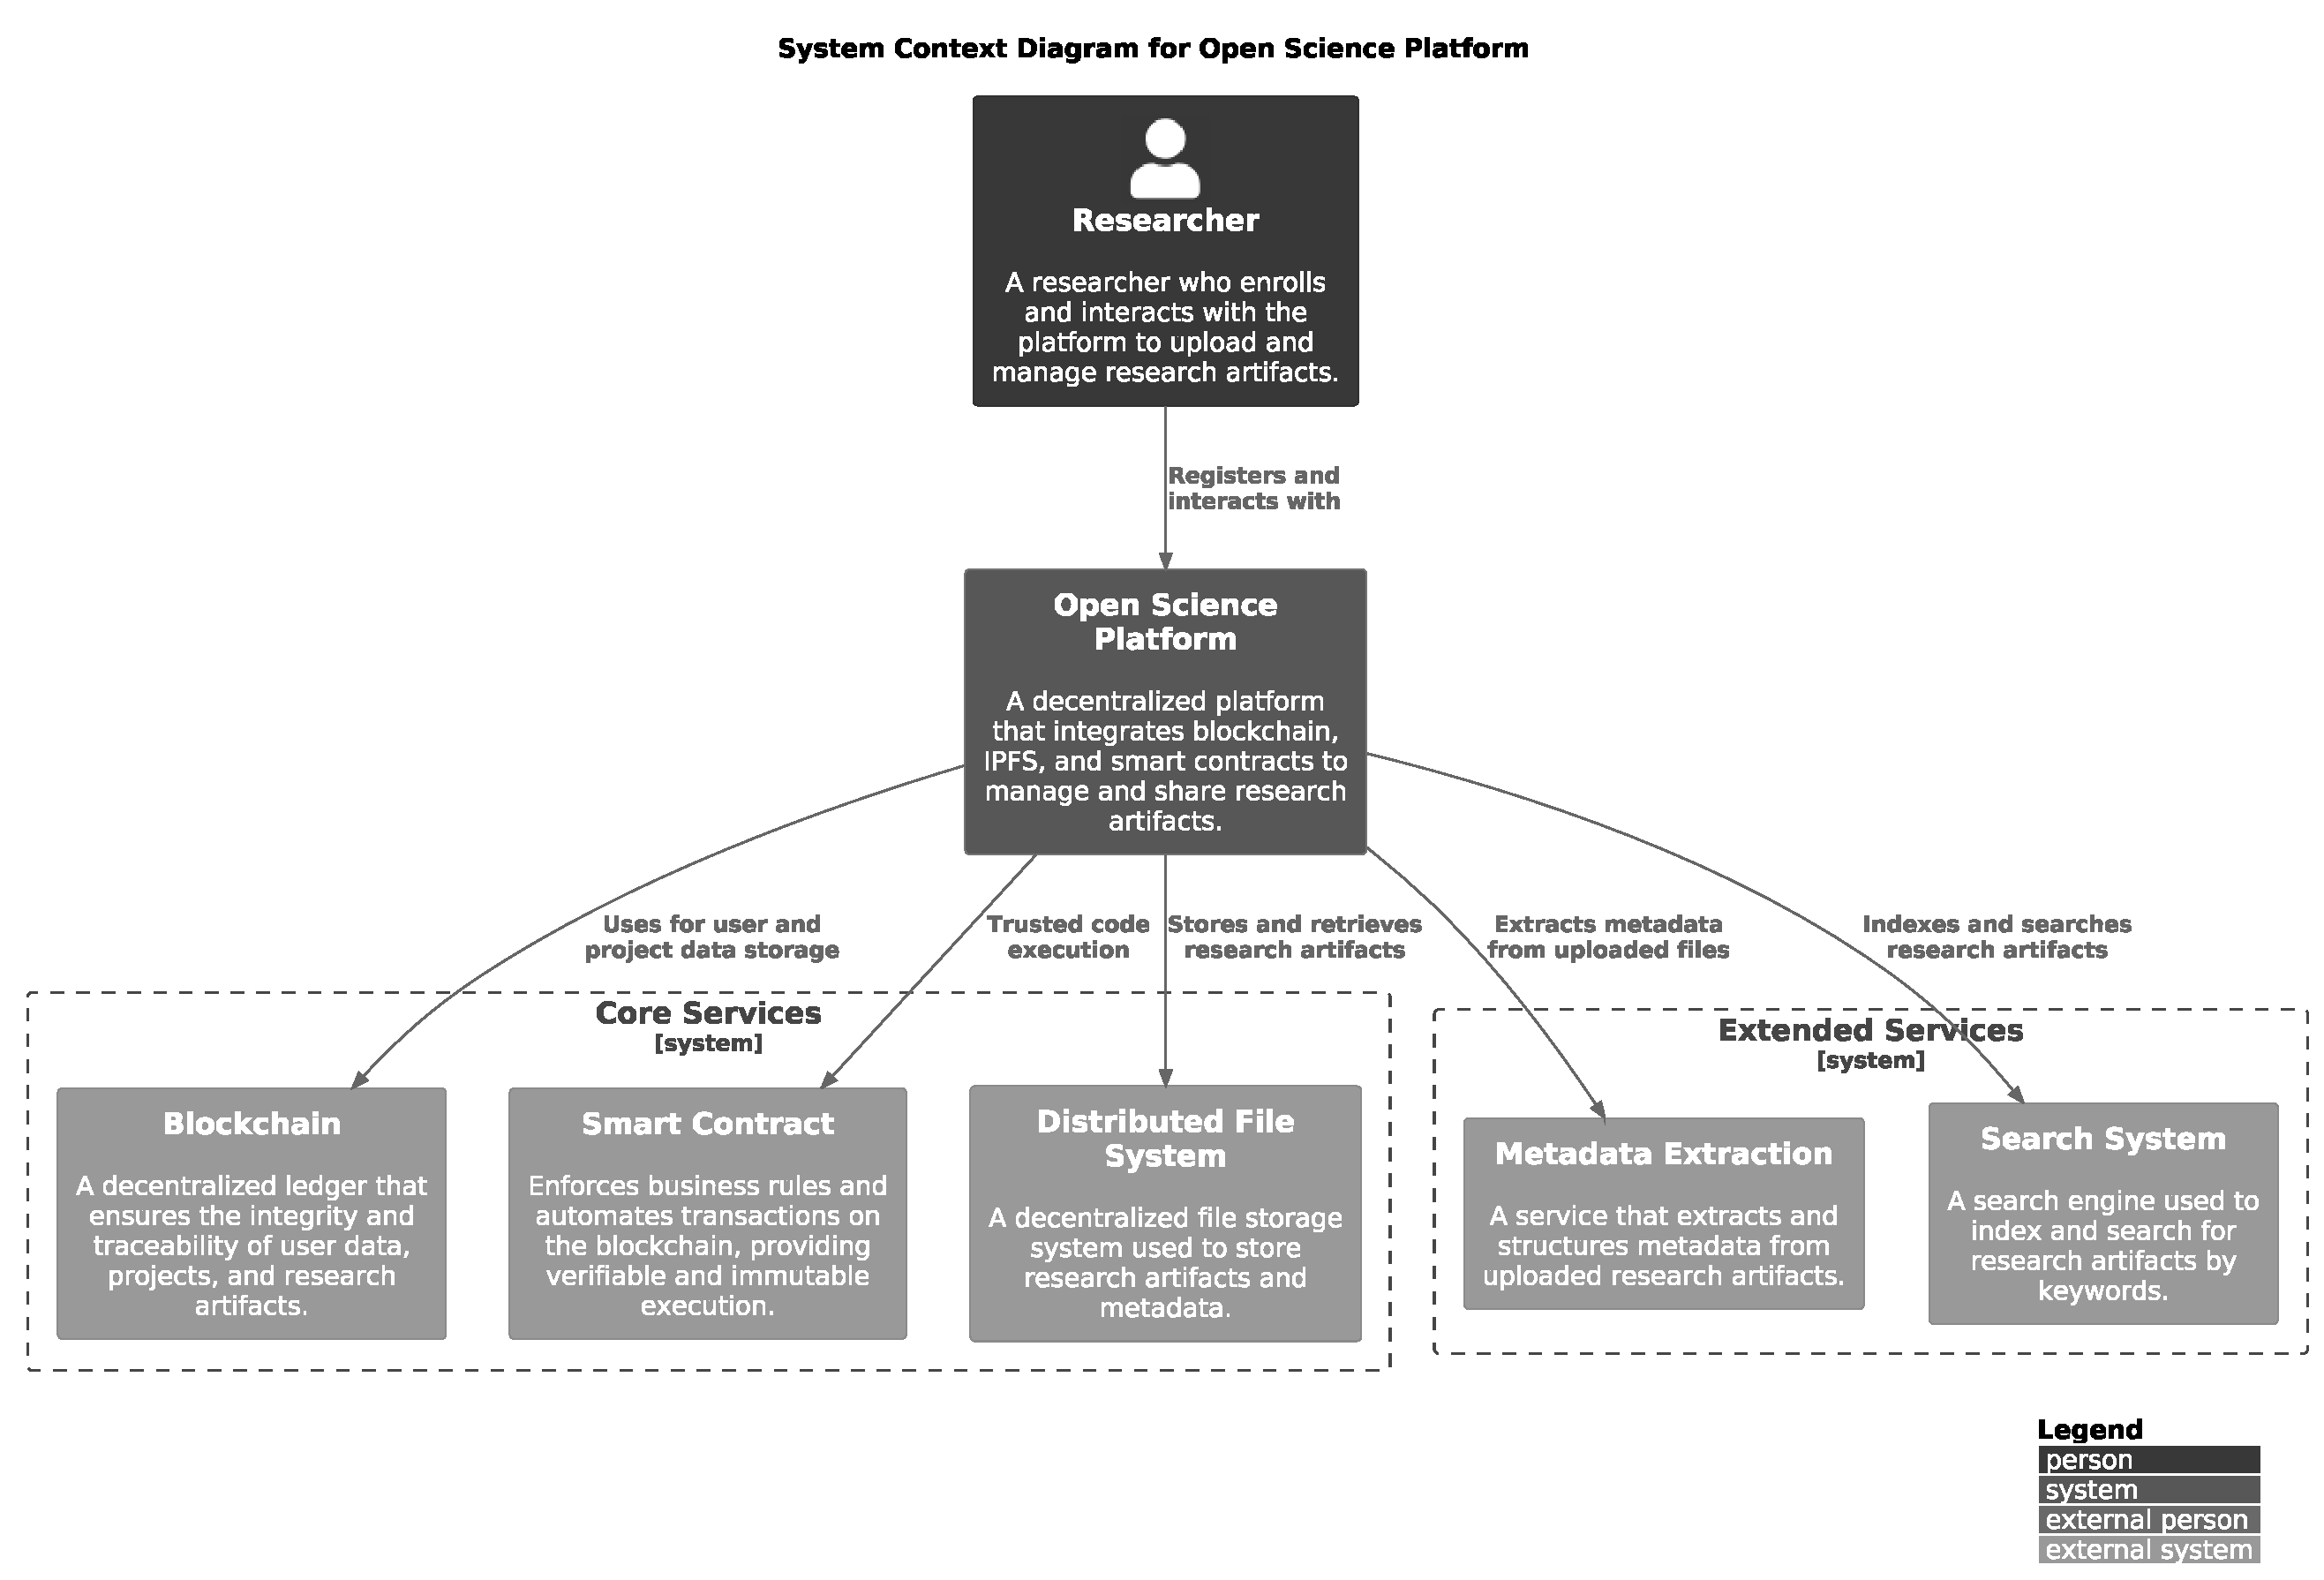
\includegraphics[width=0.98\textwidth, keepaspectratio]{fig/c4_context_diagram.eps}
    \caption{System context diagram for the Open Science Platform}
    \label{fig:c4_context_diagram}
\end{figure}



\subsection{Technology Stack}
The Open Science Platform is built on a hybrid architecture that strategically integrates decentralized and centralized components to balance security, traceability, and efficiency in data management. Decentralized technologies, such as blockchain and IPFS, ensure data integrity and tamper resistance, while centralized components facilitate indexing, search, and user interactions. Figure~\ref{fig:c4_container_diagram} presents a high-level breakdown of the platform's core building blocks.

\subsection{Core Services}

The core services of the Open Science Platform provide the fundamental infrastructure for secure and verifiable research artifact management.

\begin{itemize}
    \item \textbf{Hyperledger Iroha v1 Blockchain:} Acts as the immutable ledger for managing user and project accounts, recording transactions, and enforcing business rules via smart contracts to ensure secure and transparent data exchange.
    \item \textbf{InterPlanetary File System (IPFS):} Provides decentralized, tamper-proof storage for research artifacts and metadata, ensuring persistent and verifiable access to shared data.
\end{itemize}

\subsection{Extended Services}

The extended services enhance the platform's features by improving file and metadata processing.

\begin{itemize}
    \item \textbf{Apache Tika:} Extracts metadata from uploaded files, enhancing artifact organization and searchability.
    \item \textbf{Whoosh:} Facilitates efficient indexing and keyword-based search for stored artifacts.
\end{itemize}


\subsection{User Interface, integration and execution}

\begin{itemize}
    \item \textbf{Jupyter Notebooks (Python):} Powers the front-end interface, facilitating the automation and display of the execution steps. Blockchain interactions are managed via the Iroha v1 Python library, while communication with the IPFS network is handled through the HTTPS client library.
\end{itemize}

\begin{figure}[htbp]
    \centering
    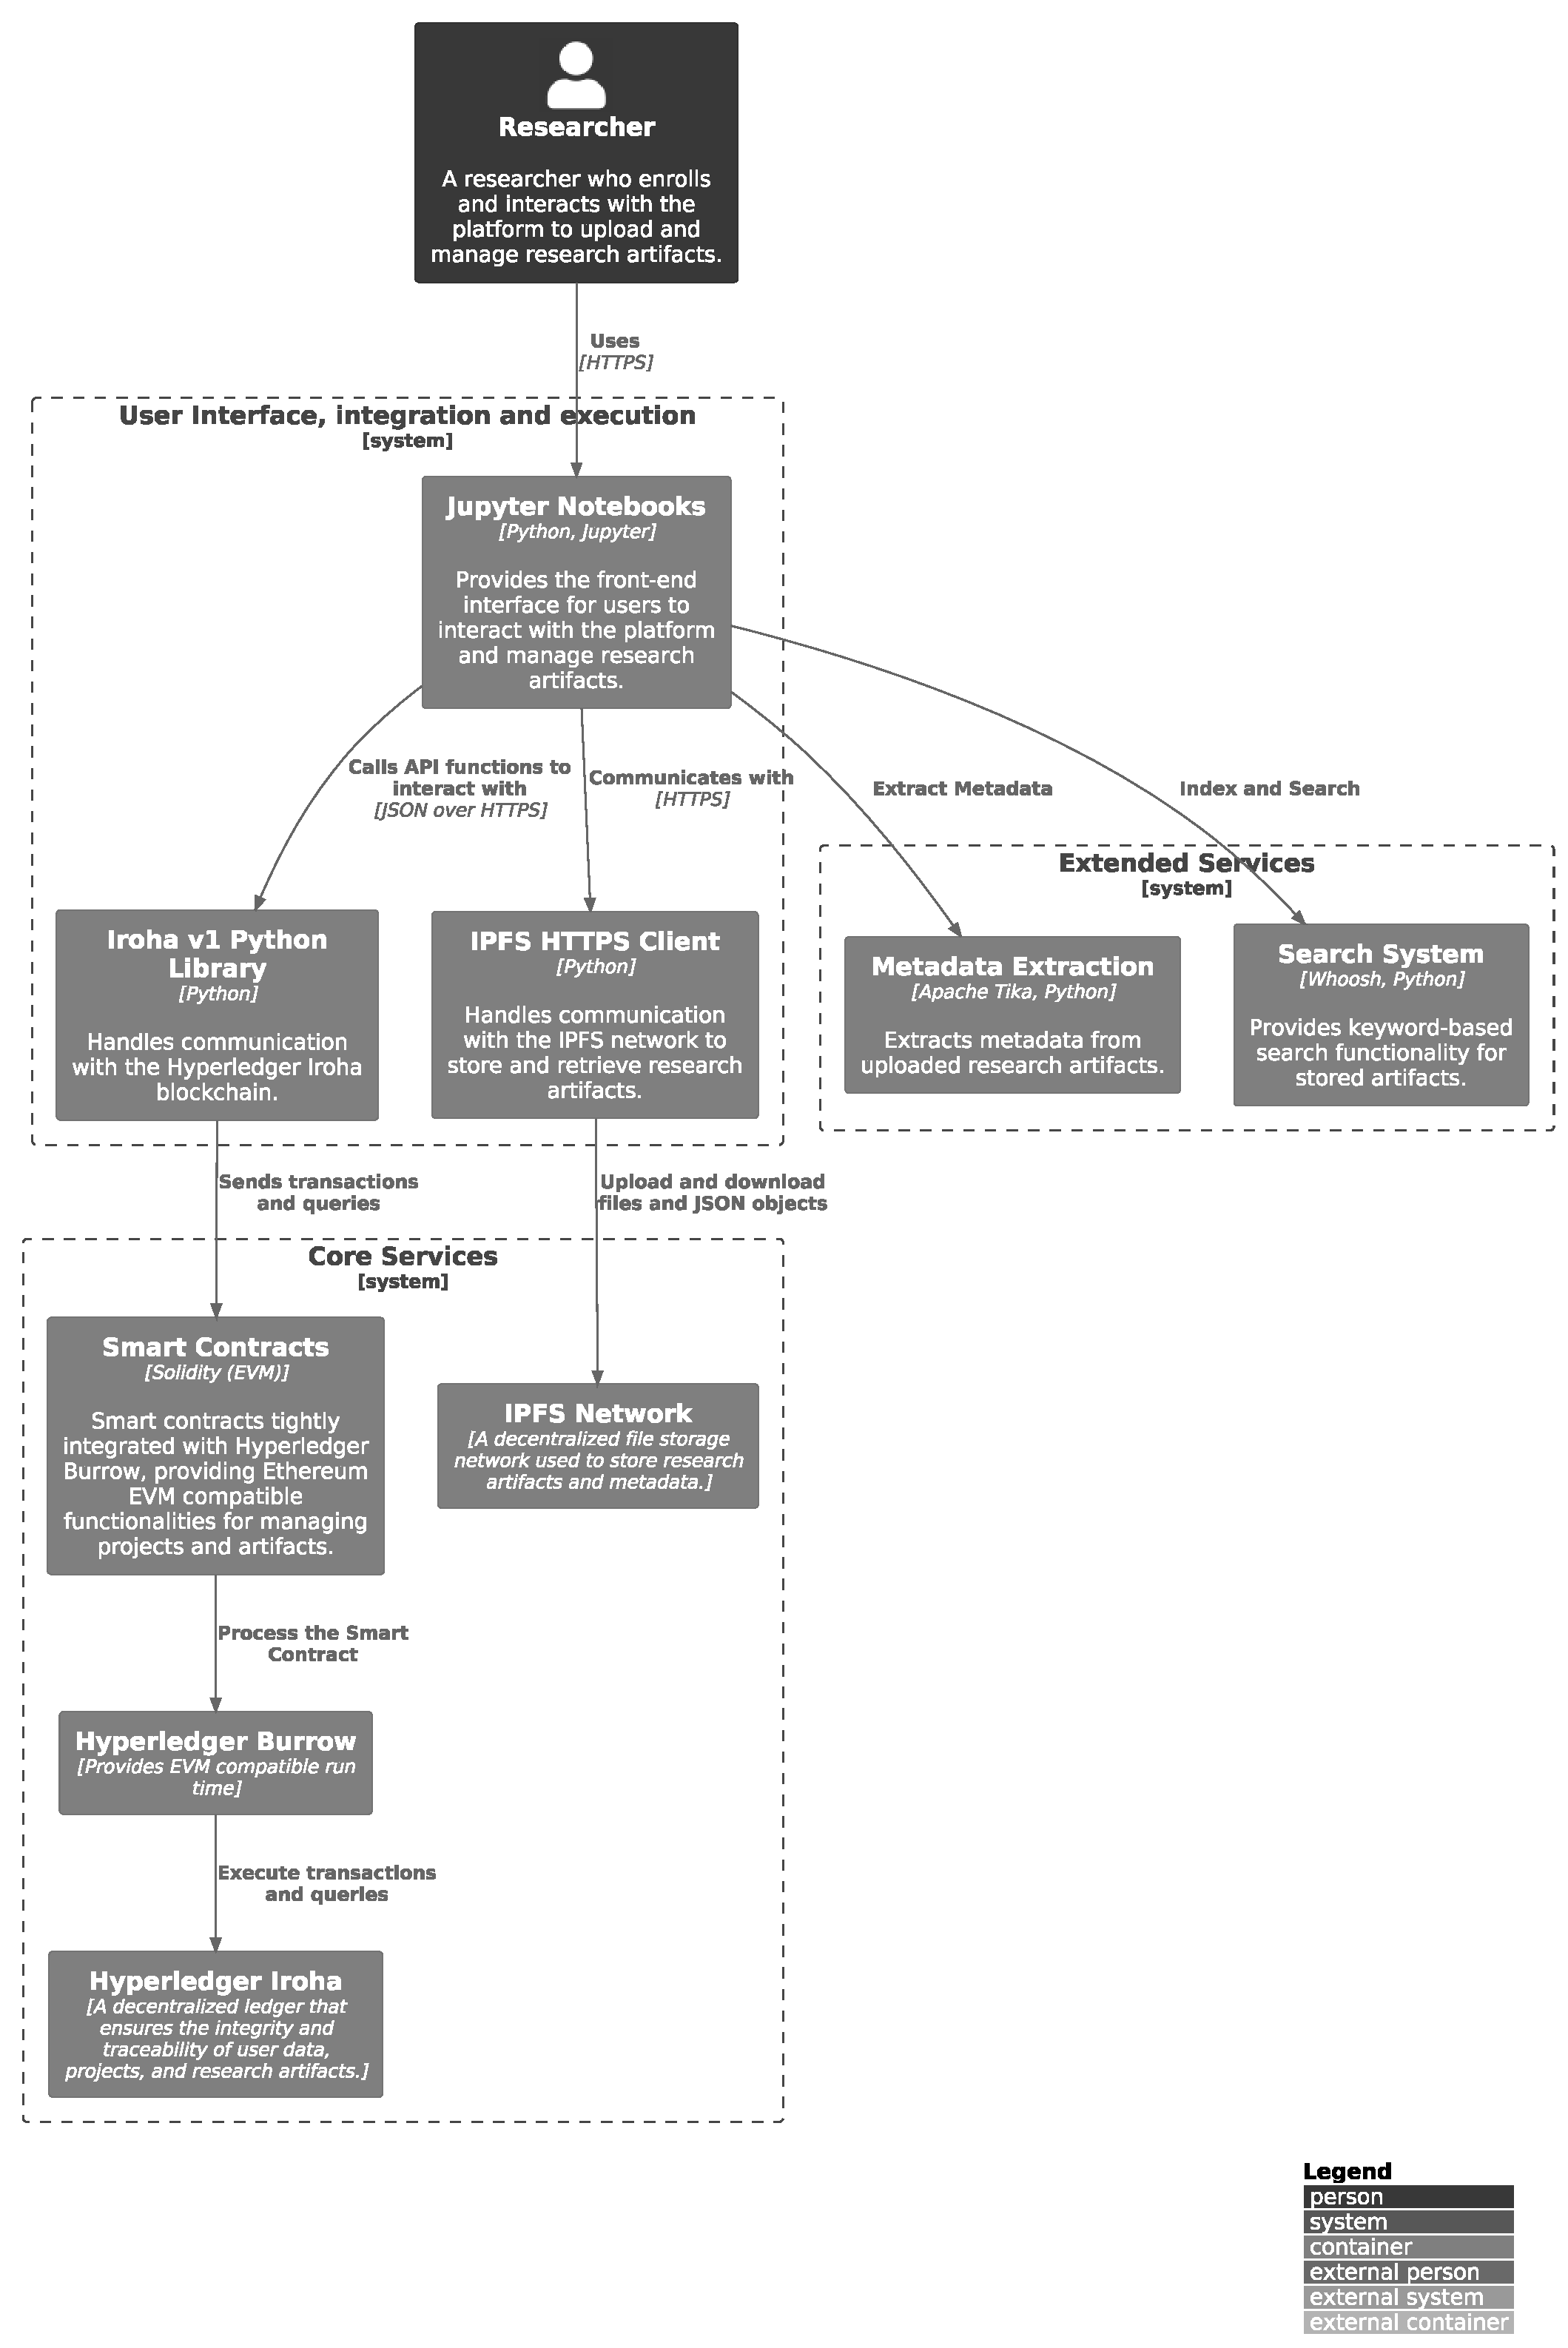
\includegraphics[width=0.98\textwidth, keepaspectratio]{fig/c4_container_diagram}
    \caption{Container diagram for the Open Science Platform}
    \label{fig:c4_container_diagram}
\end{figure}


\subsection{System Components and Interactions in the Open Science Platform}

The Open Science Platform consists of multiple interconnected components, each serving a distinct role in ensuring secure, verifiable, and reproducible research data management. The primary components include Jupyter Server, the blockchain Hyperledger Iroha v1 and the InterPlanetary File System (IPFS). Each of these elements are encapsulated within a Docker container to provide modularity, ease of deployment and reproducibility. The implementation level architecture is presented in figure~\ref{fig:c4_component_diagram}, the network topology is depicted in figure~\ref{fig:docker_ntw_topology}



\begin{figure}[htbp]
    \centering
    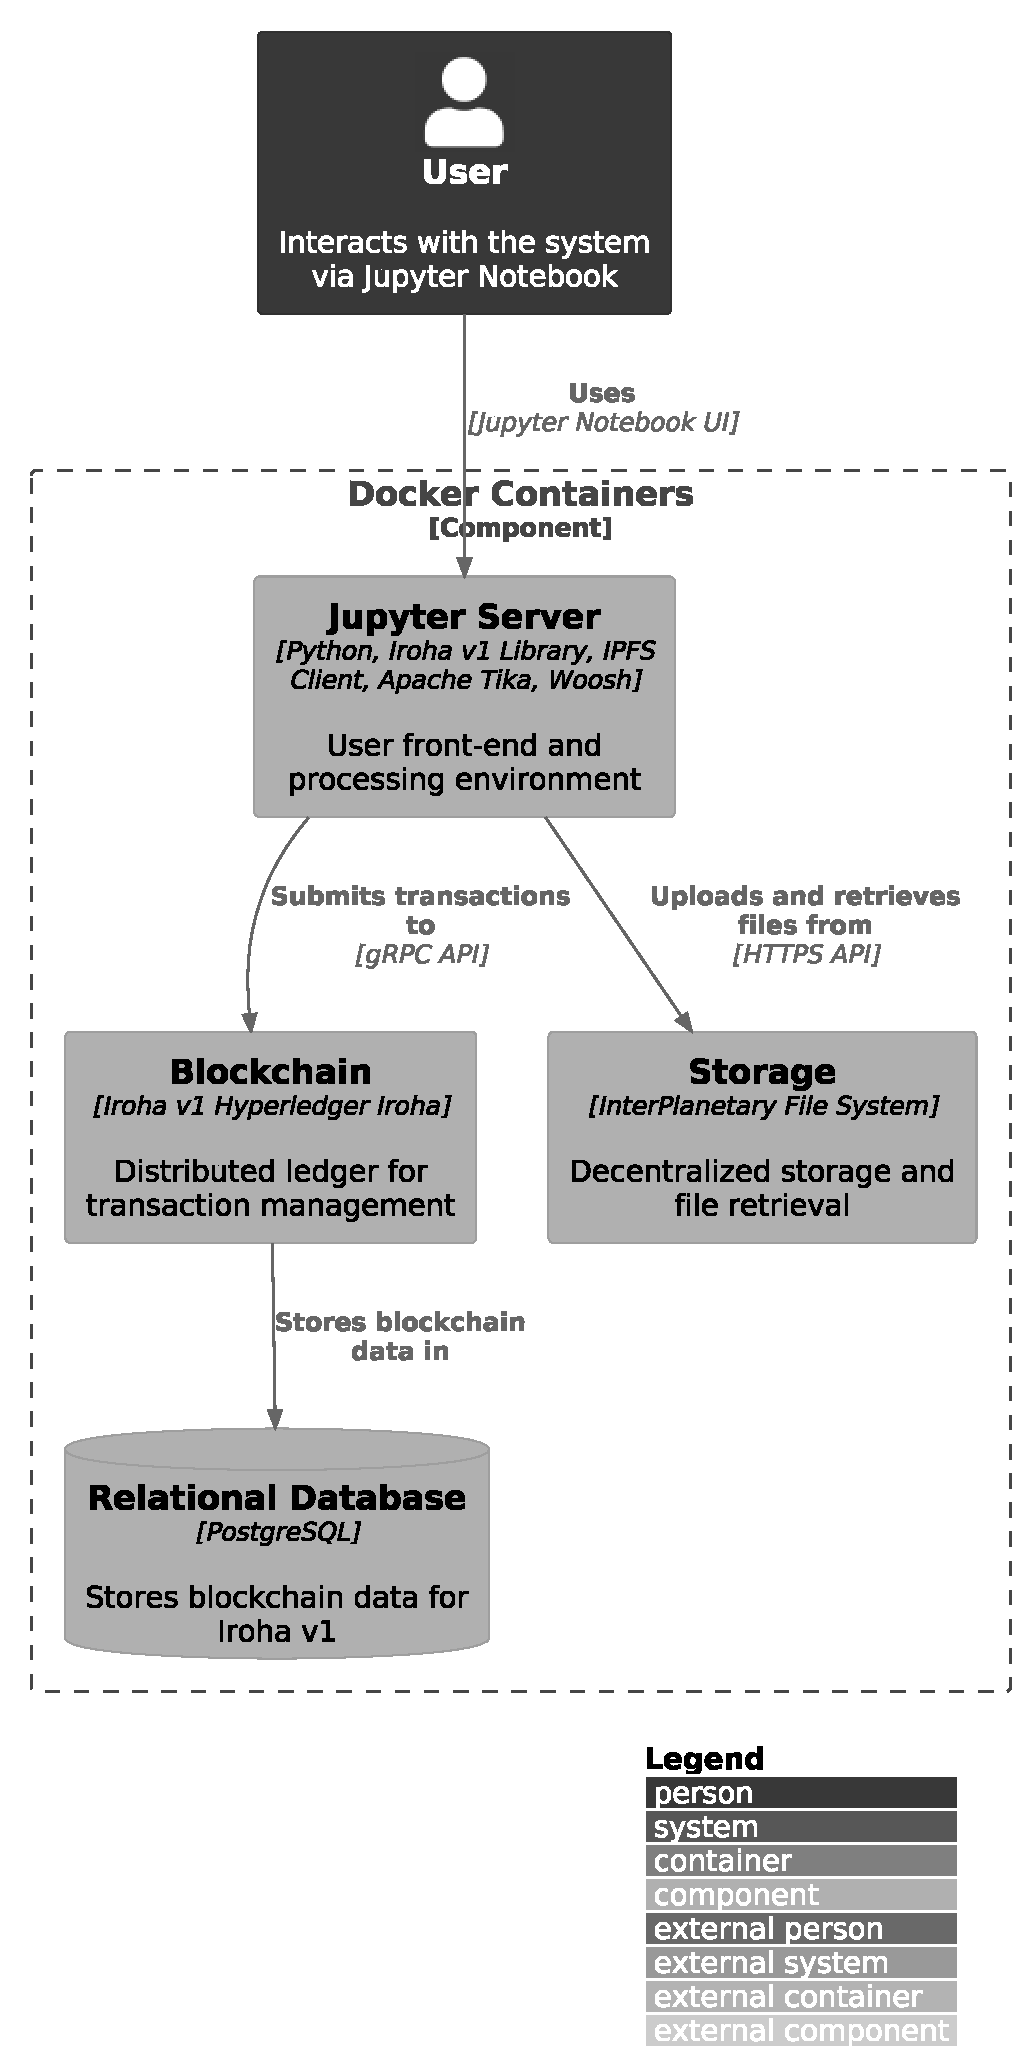
\includegraphics[width=0.98\textwidth, keepaspectratio]{fig/c4_component_diagram.eps}
    \caption{Component diagram for the Open Science Platform}
    \label{fig:c4_component_diagram}
\end{figure}


\begin{figure}[htbp]
    \centering
    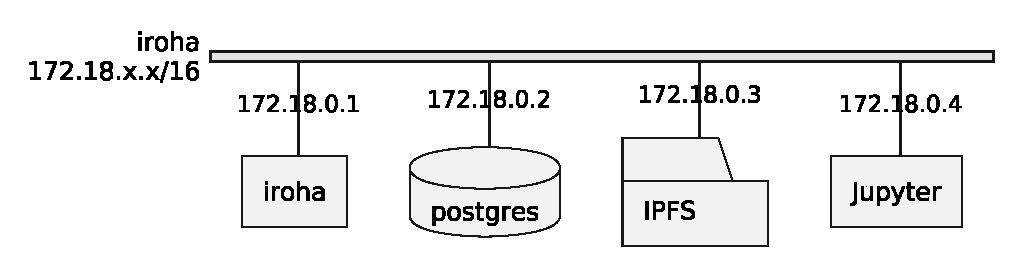
\includegraphics[width=0.98\textwidth, keepaspectratio]{fig/network_topology.eps}
    \caption{Docker network topology}
    \label{fig:docker_ntw_topology}
\end{figure}

\subsubsection{Jupyter Server}
The Jupyter Server acts as the primary interface for users interacting with the platform. This component provides a Python kernel for the execution environment that integrates the Iroha v1 Library, the IPFS HTTPS client, Apache Tika for metadata handling, and the Woosh Indexer and Search system. It enables users to:

\begin{itemize}
    \item Execute Python scripts to submit transactions and queries to the blockchain via smart contracts.
    \item Upload and retrieve files and metadata (JSON objects) stored in IPFS.
    \item Process and index research data using Apache Tika and Woosh for enhanced searchability.
    \item Access and visualize blockchain-stored metadata for Open Science applications.
\end{itemize}

\subsubsection{Blockchain}
The blockchain runs based on a Hyperledger Iroha v1 network and acts as a distributed ledger for recording transactions. It ensures immutability, transparency, and verifiability of stored research metadata. This component:
\begin{itemize}
    \item Receives transactions from the Jupyter Server via a gRPC API.
    \item Stores metadata references, ensuring that uploaded research artifacts can be authenticated.
    \item Interacts with PostgreSQL for structured storage of blockchain metadata.
    \item Supports smart contracts through the integration of Hyperledger Burrow, which provides a modular blockchain client with a permissioned smart contract interpreter partially developed to the specification of the Ethereum Virtual Machine (EVM).

\end{itemize}

\subsubsection{Storage}
The InterPlanetary File System (IPFS) is a decentralized storage solution that manages the research outputs. This component:
\begin{itemize}
    \item Stores digital research artifacts in a content-addressed manner.
    \item Allows the Jupyter Server to upload and retrieve files via an HTTPS API.
    \item Ensures long-term availability of scientific data through distributed storage principles.
\end{itemize}


\subsubsection{Relational Database (PostgreSQL)}
The PostgreSQL database provides structured storage for blockchain-related data. It is used exclusively and managed by Iroha v1 to:
\begin{itemize}
    \item Maintain an efficient and queryable record of transactions.
    \item Ensure that research metadata stored on the blockchain can be retrieved and verified.
    \item Support blockchain operations requiring fast access to structured data.
\end{itemize}

\subsubsection{Component Interactions}
The components interact in aseamless and decentralized manner:
\begin{enumerate}
    \item \textbf{User Interaction}: The user submits transactions, uploads files, and queries research data through the Jupyter Server.
    \item \textbf{Blockchain Transactions}: Jupyter Server sends and retrieves research metadata to the Iroha blockchain via gRPC API.
    \item \textbf{Metadata Storage}: Iroha stores data in the PostgreSQL database for efficient retrieval.
    \item \textbf{Decentralized Storage}: Research artifacts are stored in IPFS, with their unique file identifiers recorded on the blockchain.
    \item \textbf{File Retrieval}: Users can retrieve files from IPFS using their content identifiers (CID), ensuring authenticity and reproducibility.
\end{enumerate}

This architecture guarantees trustworthy and reproducible scientific research by leveraging blockchain for integrity, IPFS for decentralized storage, and Jupyter as an accessible research environment.





\subsection{Platform Operations}
The platform supports a set of core operations that regulate user interactions with projects and research artifacts.

\subsection{User Enrollment and Project Registration}

\sloppy
The Open Science Platform enables user enrollment and project registration, ensuring transparent and verifiable account management on the blockchain. Users self-enroll by providing cryptographic credentials and identity details, which are securely stored using a combination of blockchain attributes and decentralized storage through IPFS. Similarly, projects are registered with essential metadata, establishing a distinct blockchain account for each one. To maintain traceability and facilitate efficient project management, the system links user and project accounts bidirectionally, allowing for streamlined queries and provenance tracking. These processes are depicted in Figure~\ref{fig:c4_operations_1}.
\fussy

\begin{itemize}
    \item \textbf{User Self-Enrollment} – A user self-enrolls on the platform by providing a private key that complies with the ED25519 or SHA-3 standards and identity information, including full name, institution, email, ORCID, and role. An account is created for the user in the blockchain. All data provided in the enrollment is structured in key/value pairs into a JSON object and uploaded to IPFS, with the corresponding Content Identifier (CID) permanently linking the user’s metadata to their blockchain account.

    \item \textbf{Project Registration} – Users can register a project by specifying a descriptive name, an abstract, relevant keywords, start and end dates, funding agency, and location. Upon registration, a blockchain account is created. This data is structured in key/value pairs into a JSON object and uploaded to IPFS, with the related Content Identifier (CID) ensuring that project-related metadata remains immutable and verifiable within the blockchain.

    \item \textbf{User and Project Accounts Linkage} – Once both user and project accounts are created, the system updates their attributes to establish a bidirectional association. This ensures that querying a user account reveals linked project accounts, and vice versa, facilitating traceability and efficient project management.
\end{itemize}


\begin{figure}[htbp]
    \centering
    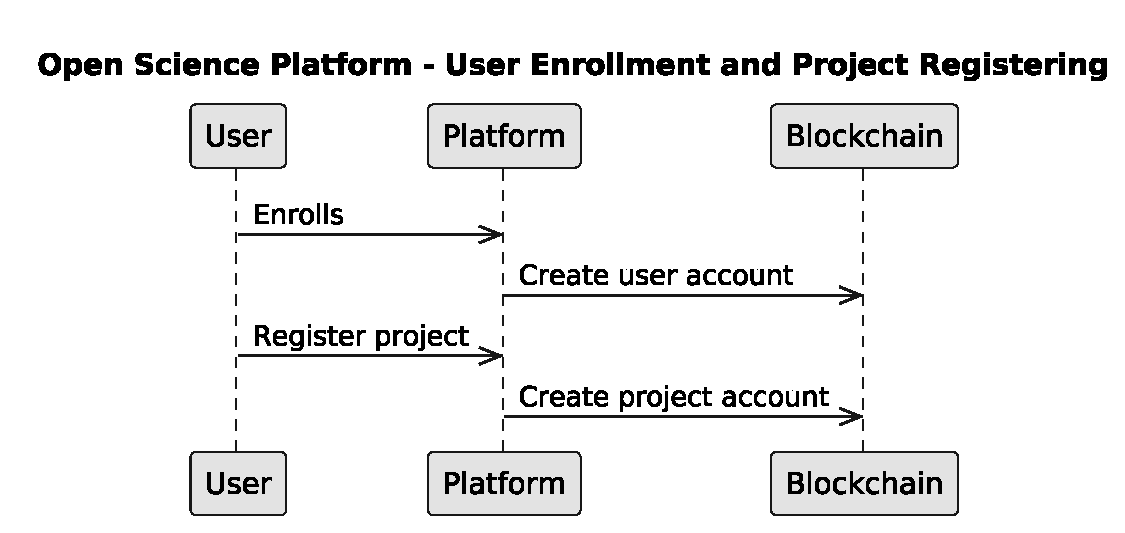
\includegraphics[scale=0.5]{fig/c4_platform_operations_1.eps}
    \caption{User enrollment and project registering for the Open Science Platform}
    \label{fig:c4_operations_1}
\end{figure}

\subsection{Artifact Management}

The Open Science Platform provides a structured approach to managing research artifacts, ensuring their integrity, traceability, and accessibility. Users can upload various types of research files, including papers, datasets, and images, which are securely stored in a decentralized manner using IPFS. Each uploaded file is assigned a unique Content Identifier (CID), which is recorded on the blockchain, creating a tamper-proof reference. To enhance discoverability, the file metadata is extracted, structured, and stored on IPFS, with its CID also registered on the blockchain. The system further supports indexing and full-text search capabilities, enabling efficient retrieval of research artifacts.

The file upload and metadata management workflow are illustrated in Figure~\ref{fig:c4_file_operations_diagram}. A user may upload research artifacts, such as papers, datasets, and images, which are stored on IPFS. Each file is assigned a unique CID, ensuring traceability and integrity, and this CID is recorded on the blockchain attributes of the corresponding project account. After upload, metadata is extracted, structured in key/value pairs, and uploaded to IPFS, with its CID also recorded on the blockchain to preserve provenance. To enhance searchability, the system indexes metadata, including full-text indexing for text-based files.

\begin{figure}[htbp]
    \centering
    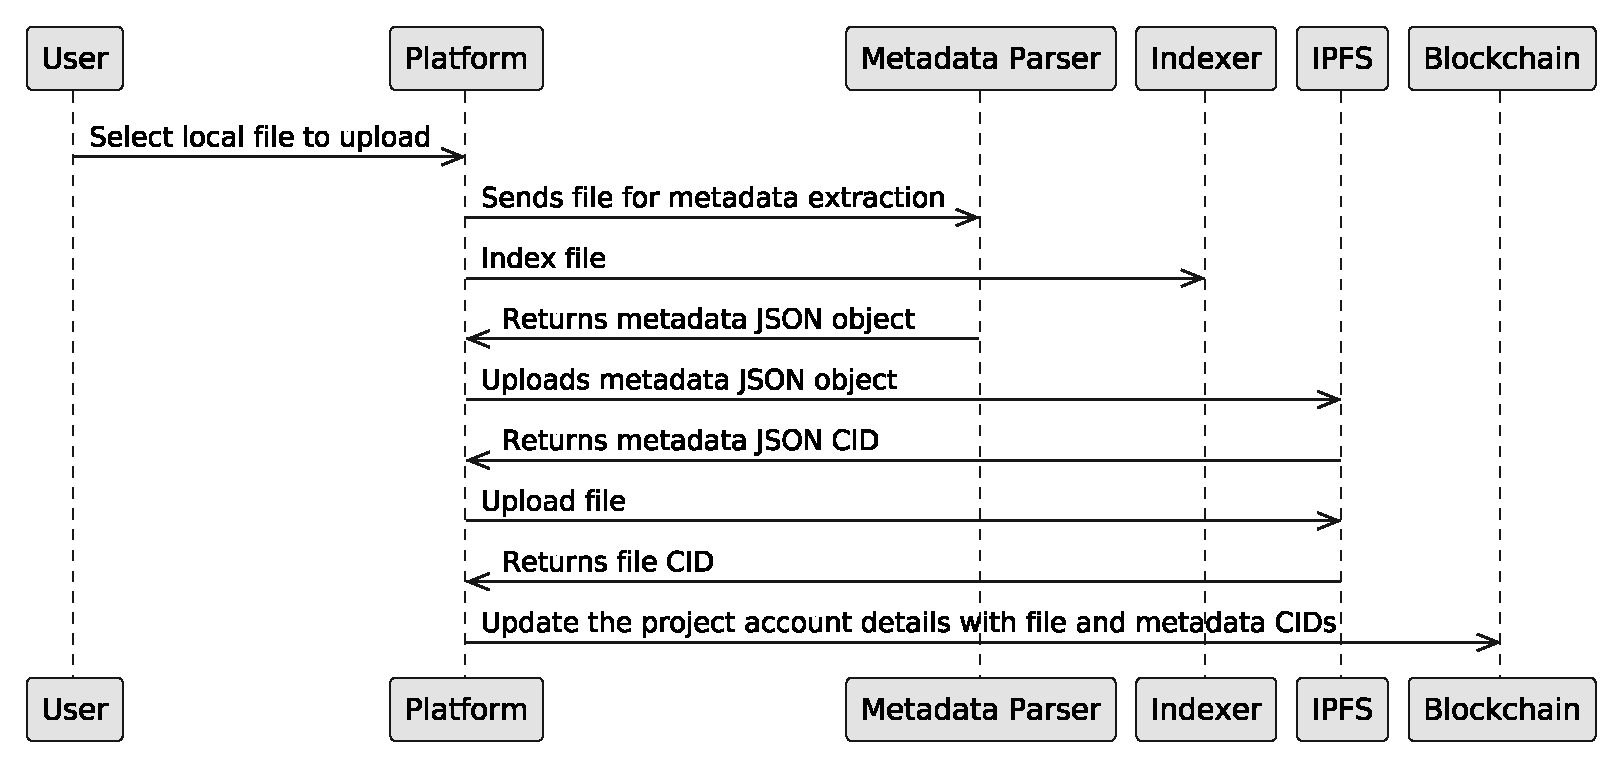
\includegraphics[width=0.98\textwidth, keepaspectratio]{fig/c4_platform_operations_2}
    \caption{File operations diagram for the Open Science Platform}
    \label{fig:c4_file_operations_diagram}
\end{figure}

The platform also enables users to search for research artifacts using keyword-based queries. As depicted in Figure~\ref{fig:c4_keyword_search}, the search engine looks up keywords in the indexed metadata and returns relevant results. Each result includes metadata details such as descriptions, subjects, and authorship, allowing users to identify relevant artifacts efficiently.

\begin{figure}[htbp]
    \centering
    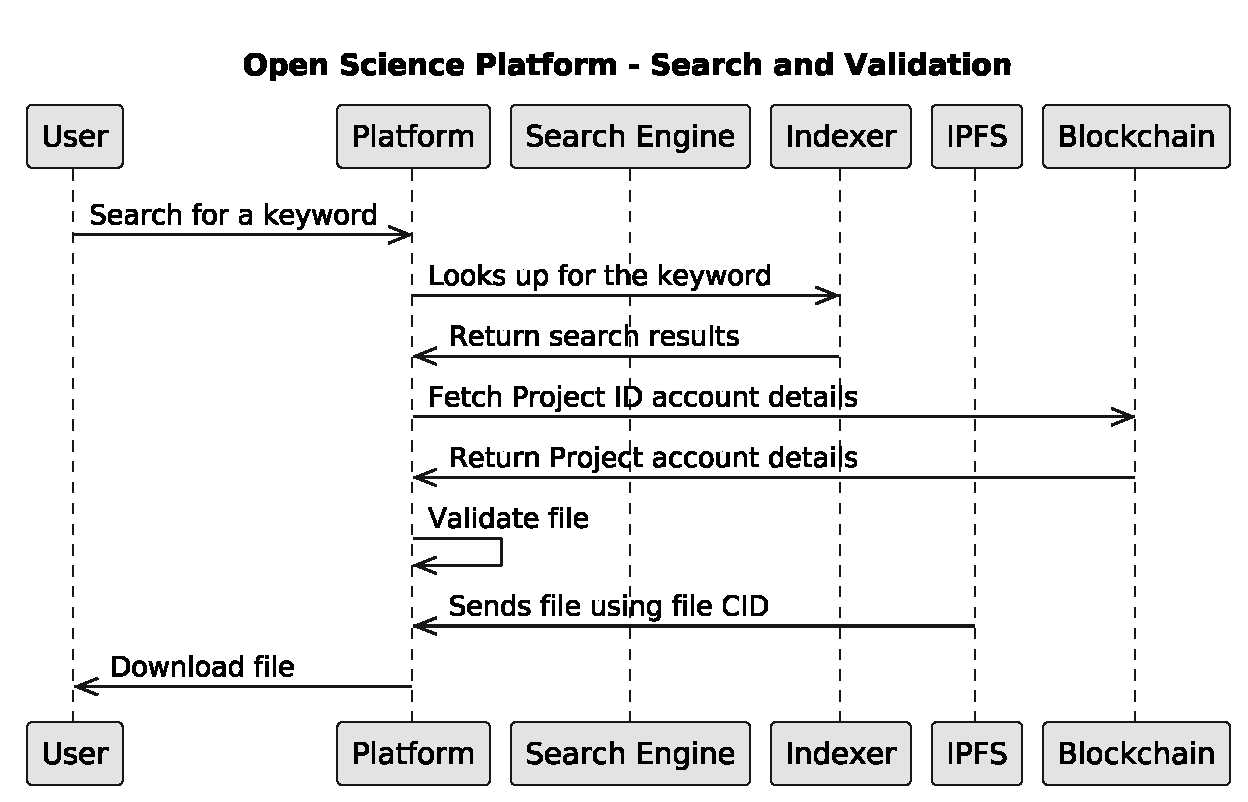
\includegraphics[width=0.98\textwidth, keepaspectratio]{fig/c4_searching_and_validation.eps}
    \caption{Keyword search, file validation, and download}
    \label{fig:c4_keyword_search}
\end{figure}

Once a file has been located, the platform performs a validation step to ensure its integrity and authenticity. The CID stored on IPFS is compared against the CID recorded on the blockchain. If they match, the file is considered valid; otherwise, the system flags it as potentially tampered with or corrupted. This validation mechanism safeguards research artifacts against unauthorized modifications. The file validation and retrieval process is depicted in figure~\ref{fig:c4_file_validation}. A validated file can then be retrieved and downloaded from IPFS to the user's local system for further use.

\begin{figure}[htbp]
    \centering
    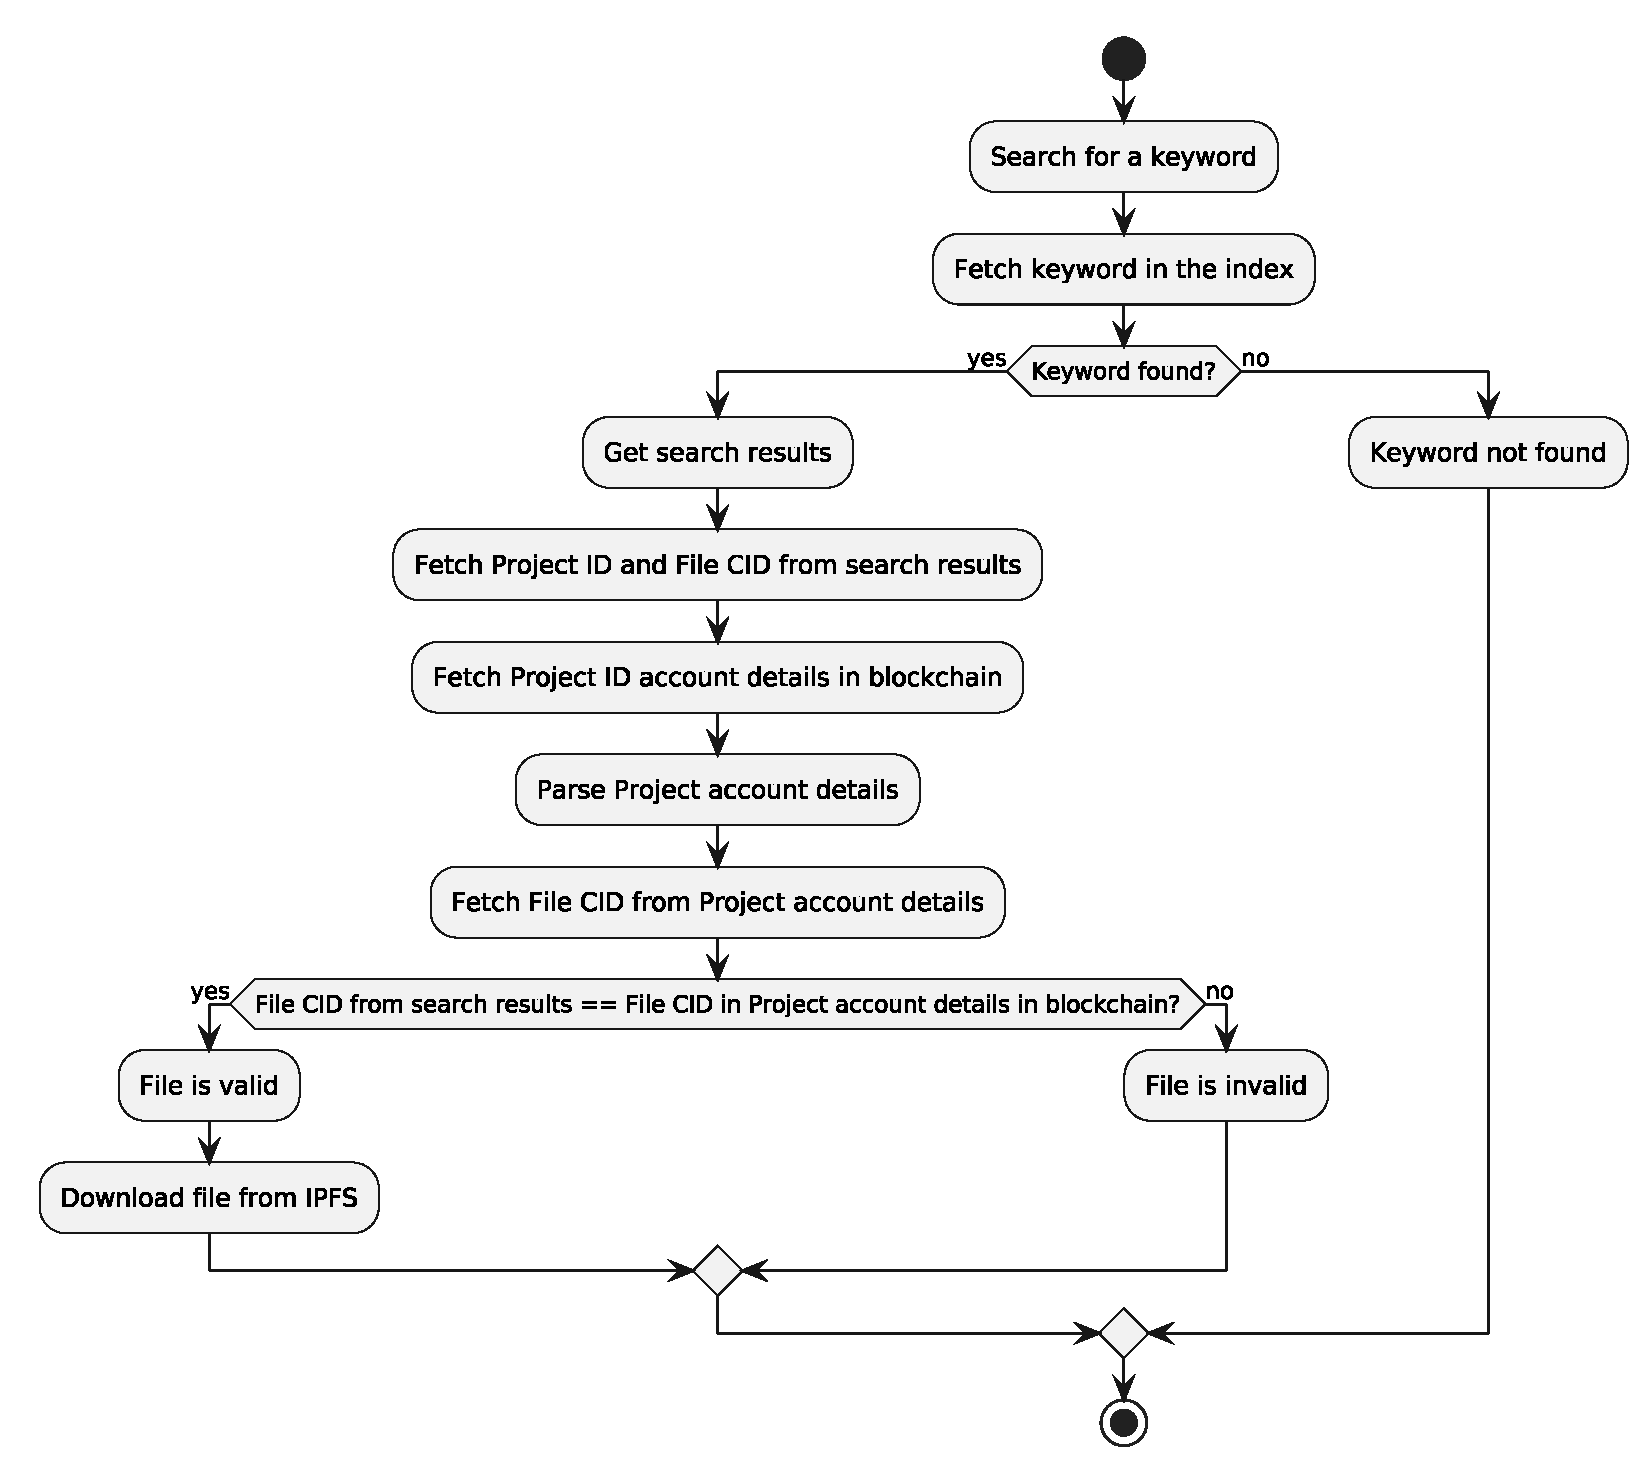
\includegraphics[width=0.98\textwidth, keepaspectratio]{fig/keyword_and_file_validation.eps}
    \caption{File validation and download}
    \label{fig:c4_file_validation}
\end{figure}



\subsection{Data Model for the Open Science Platform}

The entity-relationship model for the Open Science Platform defines the logical structure of users and research projects, capturing the associations between these entities. The primary entities in this model are \texttt{User} and \texttt{Project}, which are connected through an linked relationship, figure~\ref{fig:er_model} presents the model.


\begin{figure}[htbp]
    \centering
    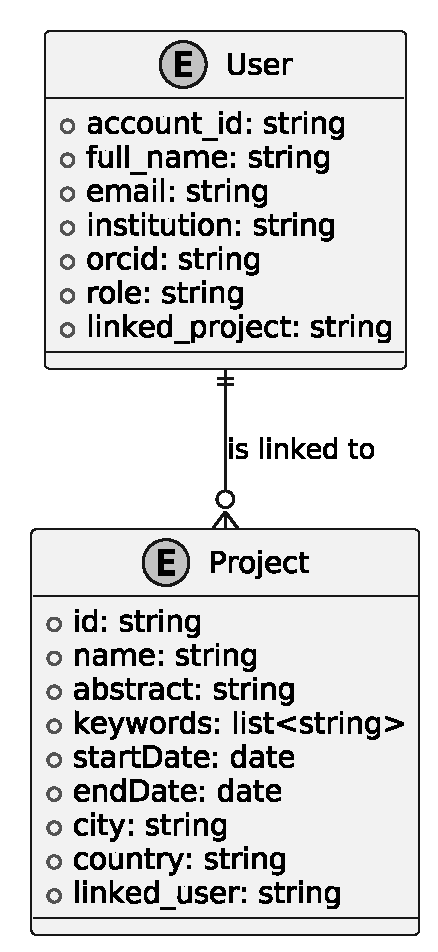
\includegraphics[width=0.98\textwidth, keepaspectratio]{fig/entity_relationship_model.eps}
    \caption{Entity-relationship model for the Open Science Platform}
    \label{fig:er_model}
\end{figure}



\subsection{User Entity}
The \texttt{User} entity represents an individual interacting with the platform. Each user is uniquely identified by an account ID and has attributes that describe personal and institutional information. The attributes of the \texttt{User} entity are listed in Table \ref{tab:user_entity}.

\begin{table}[h]
    \centering
    \renewcommand{\arraystretch}{1.2}
    \caption{User Entity Attributes}
    \label{tab:user_entity}
    \begin{tabularx}{\textwidth}{|l|X|}
        \hline
        \textbf{Attribute}       & \textbf{Description}                              \\ \hline
        \texttt{account\_id}     & A unique identifier assigned to the user.         \\ \hline
        \texttt{full\_name}      & The complete name of the user.                    \\ \hline
        \texttt{email}           & The email address used for communication.         \\ \hline
        \texttt{institution}     & The organization to which the user is affiliated. \\ \hline
        \texttt{orcid}           & The Open Researcher and Contributor ID.           \\ \hline
        \texttt{role}            & The role of the user within the research project. \\ \hline
        \texttt{linked\_project} & The research project the user is assigned to.     \\ \hline
    \end{tabularx}
\end{table}


\subsection{Project Entity}
The \texttt{Project} entity represents a research project registered in the platform. It contains essential metadata to describe the project and facilitate discovery and collaboration. The attributes of the \texttt{Project} entity are listed in Table \ref{tab:project_entity}.

\begin{table}[h]
    \centering
    \renewcommand{\arraystretch}{1.2}
    \caption{Project Entity Attributes}
    \label{tab:project_entity}
    \begin{tabularx}{\textwidth}{|l|X|}
        \hline
        \textbf{Attribute}    & \textbf{Description}                                                \\ \hline
        \texttt{project\_id}  & A unique identifier assigned to the project.                        \\ \hline
        \texttt{name}         & The official name of the project.                                   \\ \hline
        \texttt{abstract}     & A brief summary outlining the research objectives.                  \\ \hline
        \texttt{keywords}     & A list of relevant keywords associated with the project.            \\ \hline
        \texttt{startDate}    & The date when the project officially begins.                        \\ \hline
        \texttt{endDate}      & The date when the project was concluded or is expected to conclude. \\ \hline
        \texttt{city}         & The city where the project is primarily conducted.                  \\ \hline
        \texttt{country}      & The country associated with the research project.                   \\ \hline
        \texttt{linked\_user} & The user linked to the project.                                     \\ \hline
    \end{tabularx}
\end{table}


\subsection{Linked relationship between user and project enttities}
A \texttt{User} is linked to one or more \texttt{Project} entities, establishing a one-to-many relationship. This means that a single user can be associated with multiple projects. This model ensures a structured representation of research projects and their linked users, supporting an organized approach to data management in the Open Science Platform.

\subsection{ Data Model for Hyperledger Iroha v1}

The entity-relationship (ER) model of Hyperledger Iroha defines the core entities, attributes, and relationships that facilitate role-based access control, asset management, and multi-signature security. While Iroha v1 includes a broader set of entities, this research focuses solely on the account and domain related classes and attributes, as presented in figure~\ref{fig:iroha_v1_er_model}

\section{Core Entities and Their Attributes}
\subsection{Account Entity}
The \texttt{account} entity represents a user or system account registered on the blockchain. Table \ref{tab:account_entity} lists its attributes.

\begin{table}[h]
    \centering
    \renewcommand{\arraystretch}{1.2}
    \caption{Attributes of the \texttt{account} entity}
    \label{tab:account_entity}
    \begin{tabularx}{\textwidth}{|l|X|}
        \hline
        \textbf{Attribute}   & \textbf{Description}                                            \\ \hline
        \texttt{account\_id} & Unique identifier of the account                                \\ \hline
        \texttt{domain\_id}  & Links the account to a specific domain                          \\ \hline
        \texttt{quorum}      & Required number of signatories for multi-signature transactions \\ \hline
        \texttt{data}        & Stores additional metadata in JSON format                       \\ \hline
    \end{tabularx}
\end{table}


\subsection{Domain Entity}
The \texttt{domain} entity organizes accounts within logical boundaries. A \texttt{domain} can contain multiple \texttt{accounts}, as illustrated in Table~\ref{tab:domain_entity}.

\begin{table}[h]
    \centering
    \renewcommand{\arraystretch}{1.2}
    \caption{Attributes of the \texttt{domain} entity}
    \label{tab:domain_entity}
    \begin{tabularx}{\textwidth}{|l|X|}
        \hline
        \textbf{Attribute}     & \textbf{Description}                                        \\ \hline
        \texttt{domain\_id}    & Unique identifier for the domain                            \\ \hline
        \texttt{default\_role} & Default role assigned to accounts created within the domain \\ \hline
    \end{tabularx}
\end{table}



\begin{figure}[htbp]
    \centering
    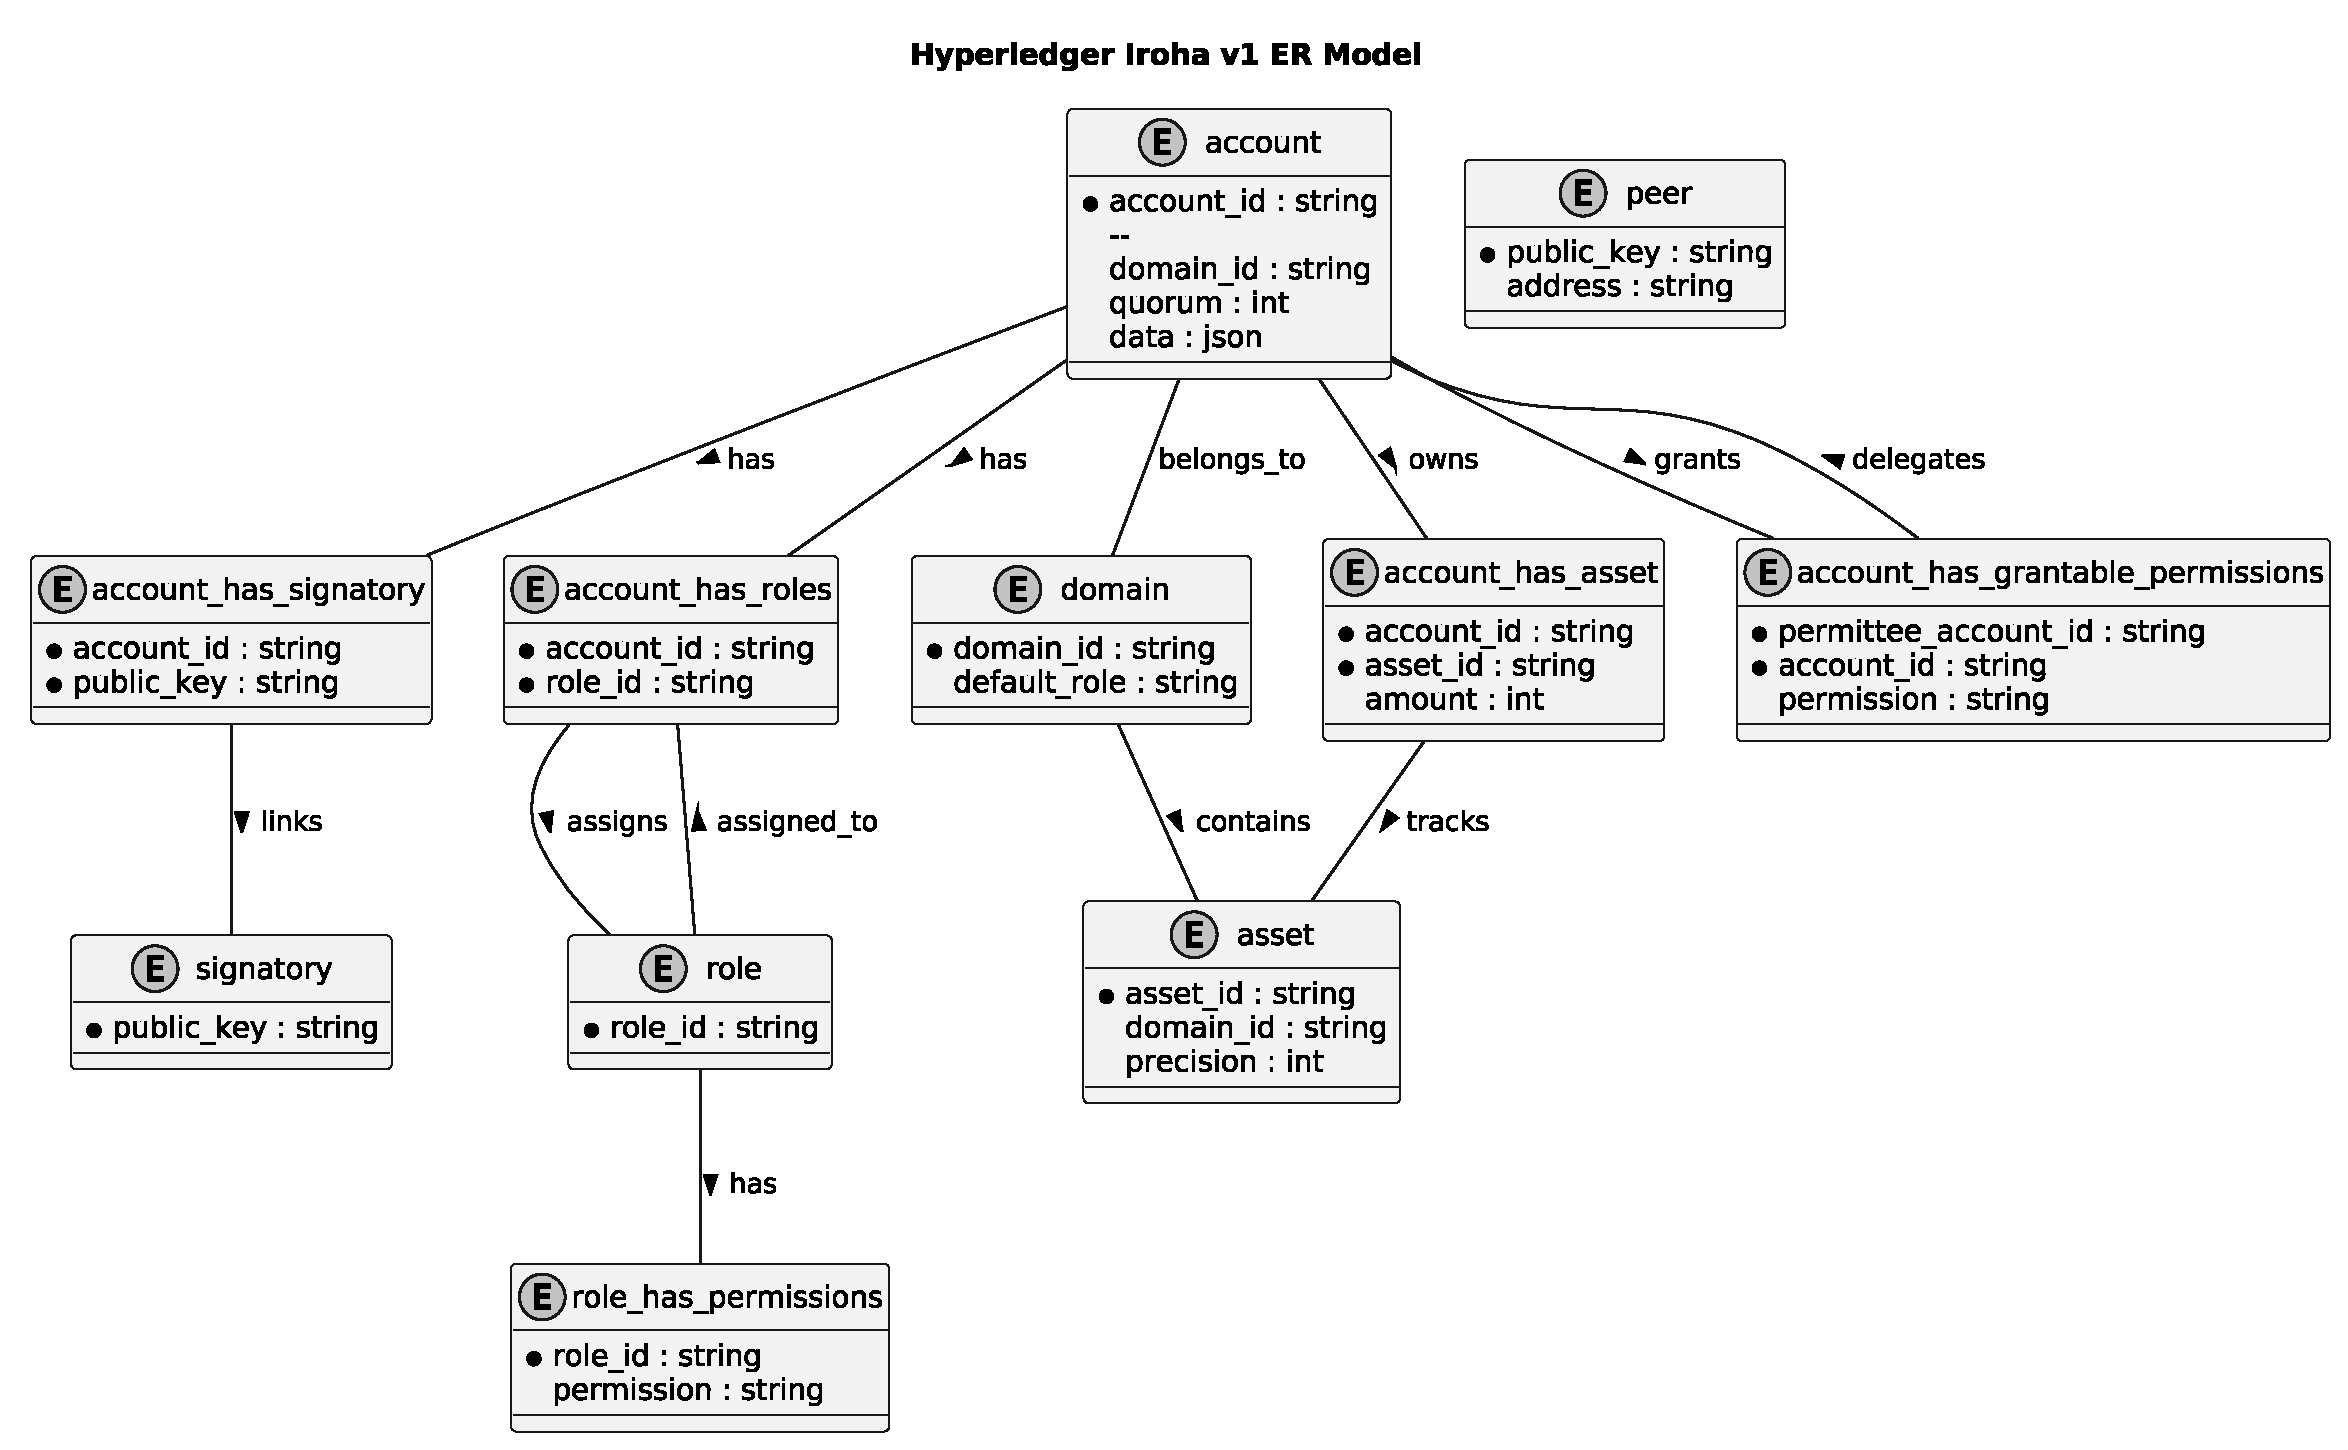
\includegraphics[width=0.98\textwidth, keepaspectratio]{fig/iroha_v1_er_model.eps}
    \caption{Subset of the Iroha v1 Entity-relationship model}
    \label{fig:iroha_v1_er_model}
\end{figure}


This ER model follows Hyperledger Iroha’s permissioned blockchain structure. It ensures fine-grained access control, multi-signature security, and domain-based account management.


\subsection{Relationship Between the Open Science Platform ER Model and the Iroha v1 ER Model}

The Open Science Platform ER model leverages the entity structure of the Iroha v1 ER model, particularly the \texttt{account} entity, to represent both the \texttt{User} and \texttt{Project} entities. In this approach, instead of introducing separate entitties for users and projects, the \texttt{account} entity in the Iroha v1 ER model serves as a general-purpose representation, encapsulating all necessary attributes in a structured format.

The attributes specific to users and projects, which are not natively present in the Iroha v1 \texttt{account} entity, are stored as JSON objects within the \texttt{data} field of the \texttt{account} entity. This design provides a flexible and scalable means of extending the entity's attributes without modifying the core schema of the Iroha blockchain.

From a relational perspective, the \texttt{account} entity maintains its standard associations with roles, permissions, and assets as defined in the Iroha v1 ER model. This ensures that user accounts and project accounts can both participate in the blockchain's permissioning system, asset ownership model, and role-based access control without requiring modifications to the underlying structure.

By reusing the \texttt{account} entity, the Open Science Platform ER model ensures compatibility with Iroha's existing mechanisms for identity management, cryptographic signing, and permission delegation. Additionally, this approach aligns with the decentralized and immutable nature of blockchain, ensuring that both user and project entities benefit from the security and transparency features inherent to the Iroha v1 framework. Figure~\ref{fig:comparing_er_models} provides a comparison between models and the rationale of use.



\begin{figure}[htbp]
    \centering
    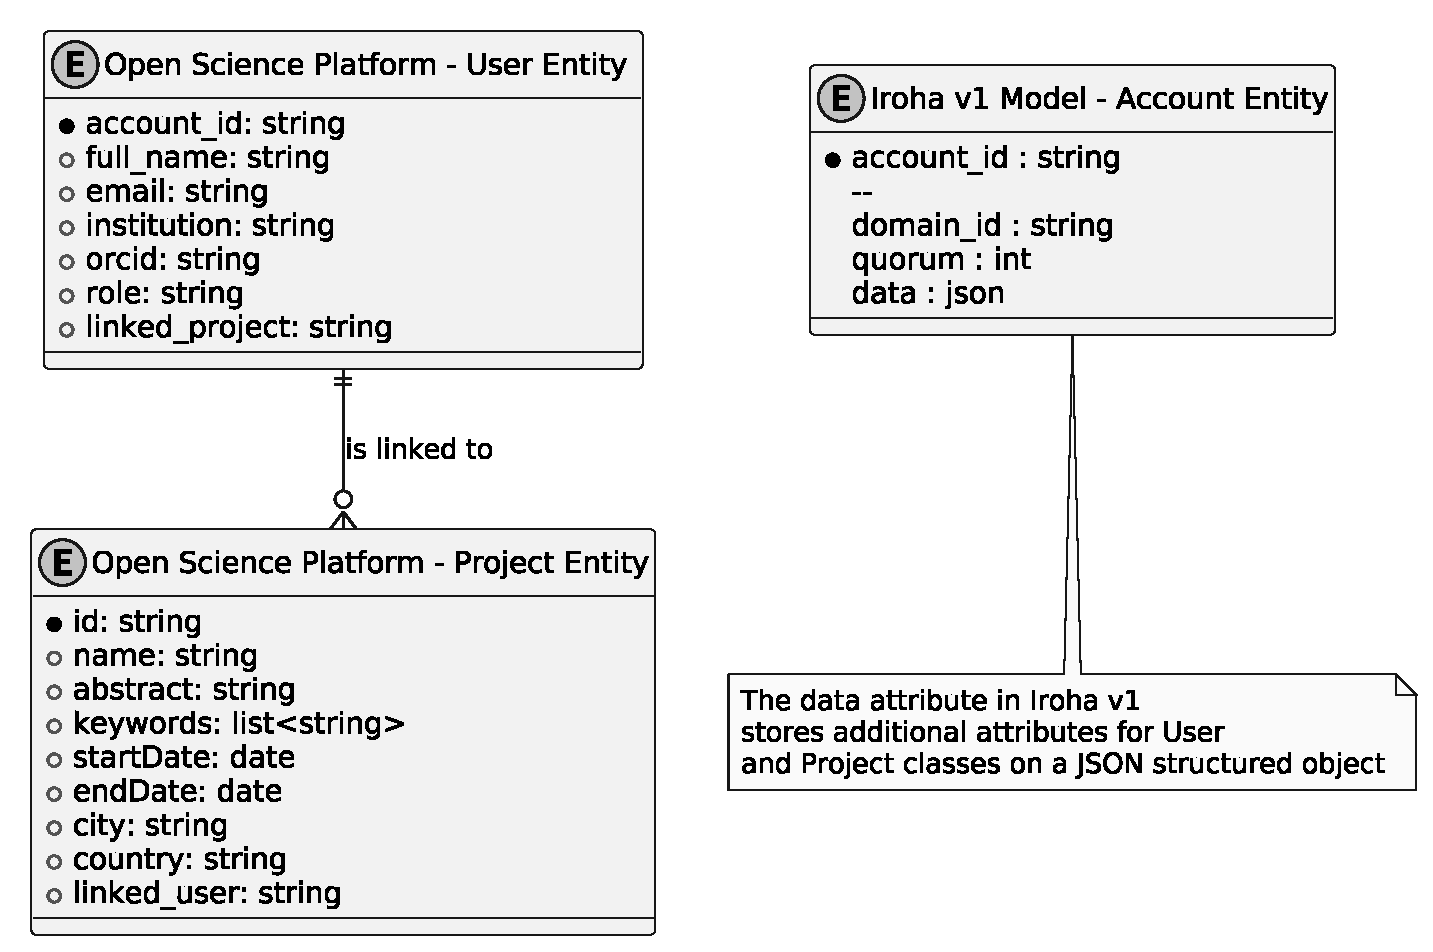
\includegraphics[width=0.98\textwidth, keepaspectratio]{fig/comparing_er_models.eps}
    \caption{Comparison of the Entitiy-relationship models}
    \label{fig:comparing_er_models}
\end{figure}


\subsection{The role of metadata and ontologies in the Open Science Platform}

Metadata plays a crucial role in both the \texttt{Account} and \texttt{Project} classes within the Open Science platform. It is used to capture and represent essential information about the user and the research project, providing context and structure to their respective data. This metadata is stored as a  JSON object, following established semantic web standards and leveraging ontologies to enhance data interoperability and accessibility.


\subsection{Selected Ontologies}
An ontology is a formal representation of knowledge as a set of concepts within a domain and the relationships between those concepts. In the context of the Open Science platform, ontologies help structure data in a way that promotes interoperability, consistency, and clarity. The use of ontologies such as \texttt{FOAF}, \texttt{Schema.org}, and \texttt{Dublin Core} ensures that data is standardized and can be easily shared and understood across different systems. These ontologies were chosen because of their widespread adoption, their ability to standardize data across different systems, and their support for rich, machine-readable representations.


\begin{table}[h]
    \centering
    \renewcommand{\arraystretch}{1.2}
    \begin{tabularx}{\textwidth}{|l|X|}            \hline
        \textbf{Ontology}                  & \textbf{Description}                                                                                                                                                                                                                                   \\ \hline
        \textbf{FOAF (Friend of a Friend)} & A vocabulary used to describe people, their activities, and their relationships to other people and objects. It is used to describe the \texttt{User} entity, including attributes like name, email, and organization.                                 \\ \hline
        \textbf{Schema.org}                & A collaborative initiative that provides a structured vocabulary for data markup on the web. It is used for describing both \texttt{User} and \texttt{Project} metadata, ensuring compatibility with web standards and promoting data discoverability. \\ \hline
        \textbf{Dublin Core (DC)}          & A metadata standard used for describing a wide range of resources, for describing the abstract, keywords, and other descriptive elements of the \texttt{Project} entity.                                                                               \\ \hline
    \end{tabularx}
    \caption{Ontologies used in the Open Science Platform}
    \label{tab:ontologies}
\end{table}


As shown in table~\ref{tab:ontologies}, by aligning with these ontologies, the platform ensures that its metadata is compatible with other Open Science initiatives and services, facilitating seamless integration and data exchange.




\subsection{User Metadata}
The metadata for the \texttt{Account} class describes the attributes associated with a user on the platform. This metadata is structured using multiple ontologies, primarily \texttt{FOAF} (Friend of a Friend) and \texttt{Schema.org}, to provide detailed and interoperable information about the user. The key attributes in the \texttt{Account} metadata include the user's name, email, organizational affiliation, unique identifier (ORCID), role, public key, and linked project.

\begin{table}[h]
    \centering
    \renewcommand{\arraystretch}{1.2}
    \begin{tabularx}{\textwidth}{|l|X|}
        \hline
        \textbf{Attribute}              & \textbf{Description}                                                                                            \\ \hline
        \texttt{foaf:name}              & The name of the user.                                                                                           \\ \hline
        \texttt{foaf:mbox}              & The email address of the user.                                                                                  \\ \hline
        \texttt{foaf:organization}      & The organization the user is affiliated with, described as an instance of the \texttt{foaf:Organization} class. \\ \hline
        \texttt{schema:identifier}      & A unique identifier for the user, such as an ORCID identifier.                                                  \\ \hline
        \texttt{foaf:holdsAccount}      & The user's account details, including their role and public key.                                                \\ \hline
        \texttt{schema:linked\_project} & The project associated with the user.                                                                           \\ \hline
    \end{tabularx}
    \caption{Account Metadata Attributes}
    \label{tab:user_metadata}
\end{table}

As presented in Table~\ref{tab:user_metadata}, this structured metadata helps ensure the user information is standardized and interoperable across different systems and platforms.


\subsection{The use of JSON-LD for metadata representation}

JSON for Linked Data (JSON-LD) is a lightweight Linked Data format designed to structure and interconnect data on the web using standard JSON. It extends JSON by incorporating semantic web principles, making data more discoverable, reusable, and machine-readable. JSON-LD achieves this by including a \texttt{@context} element, which maps terms to well-defined ontologies, and a \texttt{@graph} element, which structures entities and their relationships in a linked data format.

A key advantage of JSON-LD is its compatibility with existing JSON-based systems while enabling seamless integration with the semantic web. By leveraging vocabularies such as Schema.org and Dublin Core, JSON-LD ensures interoperability across diverse platforms and datasets. This makes it particularly useful for Open Science applications, where structured metadata enhances research reproducibility and data sharing.

In the context of the Open Science platform, JSON-LD is used to encode metadata for users and research projects, ensuring alignment with widely accepted ontologies. The structured representation enables automatic indexing, metadata enrichment, and semantic search capabilities, facilitating better knowledge discovery and integration within the scientific community.


\subsection{The User Metadata JSON-LD object}

The user metadata is structured using two primary ontologies: Friend of a Friend (FOAF) and Schema.org.

The FOAF ontology is used to describe personal and organizational attributes of users within the platform. It provides well-defined properties such as \texttt{foaf:name} for the user’s full name, \texttt{foaf:mbox} for email addresses, and \texttt{foaf:organization} for institutional affiliations. By leveraging FOAF, the platform ensures standardized representation of user identities and their associations, facilitating integration with other systems that utilize FOAF-based user profiles.

Schema.org complements FOAF by enriching the user metadata with structured properties that enhance discoverability and machine readability. The \texttt{schema:identifier} property, for instance, is used to store unique user identifiers such as ORCID, ensuring compatibility with global researcher identification systems. Additionally, \texttt{schema:roleName} captures the user’s role within the platform (e.g., reviewer, publisher), while \texttt{schema:publicKey} stores cryptographic keys associated with the user’s account. The \texttt{schema:linked\_project} property establishes connections between users and their associated research projects, enabling efficient metadata retrieval and knowledge graph construction as exhibited in Figures~\ref{jsonld:user} and ~\ref{fig:user_metadata}, the JSON-LD structure represents the project metadata in the Open Science platform.


\begin{figure}[h]
    \centering
    \caption{JSON-LD structure for user metadata in the Open Science platform}
    \label{jsonld:user}
    \begin{verbatim}
  {
      "@context": {
          "schema": "http://schema.org/",
          "foaf": "http://xmlns.com/foaf/0.1/"
      },
      "@graph": [
          {
              "@type": "foaf:Person",
              "foaf:name": "Zealous Ptolemy",
              "foaf:mbox": "zealous_ptolemy@email.com",
              "foaf:organization": {
                  "@type": "foaf:Organization",
                  "foaf:name": "Ashkelon Academic College"
              },
              "schema:identifier": {
                  "@type": "PropertyValue",
                  "propertyID": "ORCID",
                  "value": "6153-7096-0437-X"
              },
              "foaf:holdsAccount": {
                  "schema:identifier": "zealous_ptolemy@test",
                  "schema:roleName": "reviewer",
                  "schema:publicKey": "ca4c00c0a43bbd2caf070ab780886906ebb70e2c3d975972ccab4e15c01f33bd"
              },
              "schema:linked_project": "02226@test"
          }
      ]
  }
  \end{verbatim}
\end{figure}


\begin{figure}[htbp]
    \centering
    \includegraphics[width=0.98\textwidth, keepaspectratio]{fig/user_metadata.eps}
    \caption{User metadata}
    \label{fig:user_metadata}
\end{figure}



By combining FOAF and Schema.org, the Open Science platform ensures that user metadata is both human-readable and machine-actionable, promoting seamless integration with external research infrastructures and fostering an interoperable ecosystem for Open Science.

\subsection{The Project Metadata JSON-LD object}

The metadata for the \texttt{Project} entity provides essential details about the research project hosted on the platform. Similar to the \texttt{User} metadata, the project metadata is structured using \texttt{Schema.org} and \texttt{Dublin Core} (\texttt{dc}) ontologies. This structure allows for a comprehensive description of the project, including its name, abstract, keywords, timeline, funding details, and location.

\begin{table}[h]
    \centering
    \label{tab:project_metadata}
    \renewcommand{\arraystretch}{1.2}
    \begin{tabularx}{\textwidth}{|l|X|}
        \hline
        \textbf{Attribute}           & \textbf{Description}                                                                                           \\ \hline
        \texttt{schema:name}         & The name of the research project.                                                                              \\ \hline
        \texttt{dc:abstract}         & A brief abstract describing the project's objectives and focus.                                                \\ \hline
        \texttt{schema:keywords}     & Keywords associated with the project, such as "precision agriculture" and "global supply chains."              \\ \hline
        \texttt{schema:startDate}    & The start date of the project.                                                                                 \\ \hline
        \texttt{schema:endDate}      & The end date of the project.                                                                                   \\ \hline
        \texttt{schema:funding}      & The funding organization for the project, described as an instance of the \texttt{schema:Organization} class.  \\ \hline
        \texttt{schema:location}     & The physical location where the project is based, described as an instance of the \texttt{schema:Place} class. \\ \hline
        \texttt{schema:metadataCID}  & A unique identifier for the metadata of the project.                                                           \\ \hline
        \texttt{schema:linked\_user} & The user associated with the project.                                                                          \\ \hline
    \end{tabularx}
    \caption{Project Metadata Attributes}
\end{table}

The following JSON structure describes the metadata for a \texttt{Project} in the Open Science platform as shown in Figures~\ref{jsonld:project} and ~\ref{fig:project_metadata}.


\begin{figure}[h]
    \centering
    \caption{JSON-LD structure for project metadata in the Open Science platform}
    \label{jsonld:project}
    \begin{verbatim}
  {
      "@context": {
          "schema": "http://schema.org/",
          "dc": "http://purl.org/dc/terms/"
      },
      "@graph": [
          {
              "@type": "schema:ResearchProject",
              "schema:identifier": "02226@test",
              "schema:publicKey": "1c6b8d00c8382c93eb0dd3eeb24a20bfece56a28326bbaebb647cadaf4750520",
              "schema:description": {
                  "@context": {
                      "schema": "http://schema.org/",
                      "dc": "http://purl.org/dc/terms/"
                  },
                  "@type": "schema:ResearchProject",
                  "schema:name": "Assessing the Benefits of precision agriculture for global supply chains",
                  "dc:abstract": "This research focuses on the benefits and challenges posed by precision agriculture for global supply chains, with an emphasis on its potential for disease prevention.",
                  "schema:keywords": [
                      "precision agriculture",
                      "global supply chains",
                      "disease prevention"
                  ],
                  "schema:startDate": "2023-12-18",
                  "schema:endDate": "2027-01-02",
                  "schema:funding": {
                      "@type": "schema:Organization",
                      "schema:name": "World Wildlife Fund"
                  },
                  "schema:location": {
                      "@type": "schema:Place",
                      "schema:name": "Los Angeles, California, USA"
                  }
              },
              "schema:metadataCID": "Qmay4cDaxUaZaHoJKqzN69XkiX8wMx17aG4VMmwmkLcL1a",
              "schema:linked_user": "zealous_ptolemy@test"
          }
      ]
  }
  \end{verbatim}
\end{figure}



\begin{figure}[htbp]
    \centering
    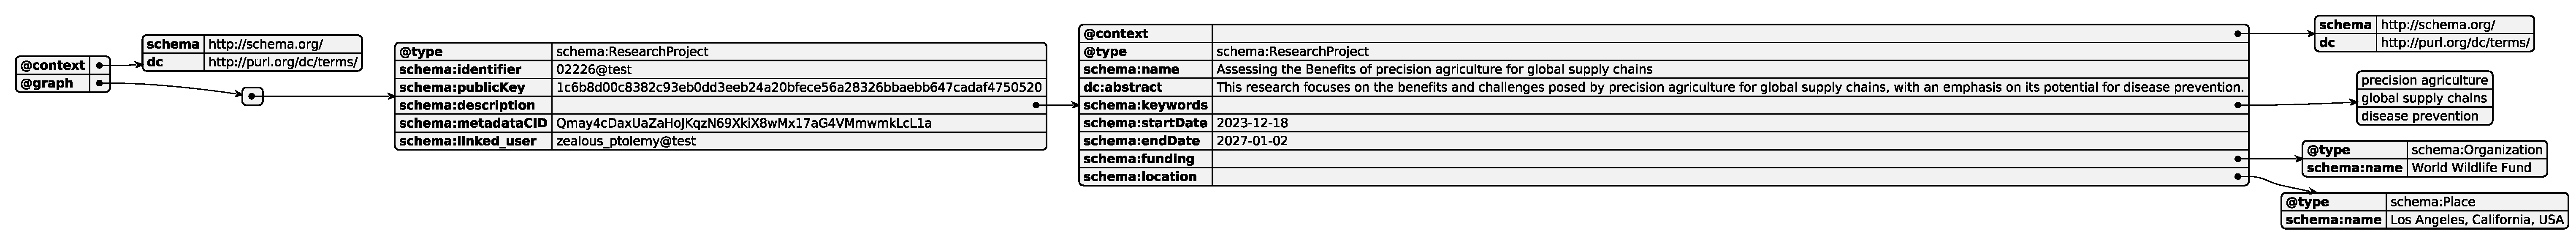
\includegraphics[width=0.98\textwidth, keepaspectratio]{fig/project_metadata.eps}
    \caption{Project metadata}
    \label{fig:project_metadata}
\end{figure}


This metadata not only captures the essential details of the project but also ensures that these details are linked to the user's profile, making it easier to track the relationship between users and their associated research efforts.


\subsection{General Metadata Handling Workflow}

The Open Science platform follows a general approach to metadata handling, ensuring that it is properly formatted, stored, and made immutable through blockchain integration. The process begins with processing the relevant metadata, which may pertain to a user, project, or file. This metadata is then formatted according to the JSON-LD standard, ensuring semantic interoperability and alignment with established ontologies.

Once formatted, the JSON-LD object is sent to the InterPlanetary File System (IPFS), a decentralized storage solution that provides content-addressable storage. Upon successful storage, IPFS generates a unique Content Identifier (CID) that serves as a reference to the stored metadata. This CID is then recorded on the blockchain by writing it into the account details associated with the entity. By anchoring the metadata CID on the blockchain, the platform ensures integrity, immutability, and transparency.

Finally, the blockchain transaction containing the CID serves as a provenance record, allowing stakeholders to verify and trace metadata modifications over time. The entire workflow guarantees that metadata remains both accessible and verifiable, promoting reproducibility and trust within the Open Science ecosystem.

Figure~\ref{fig:metadata_workflow} illustrates the sequence of operations in the metadata handling process.


\begin{figure}[htbp]
    \centering
    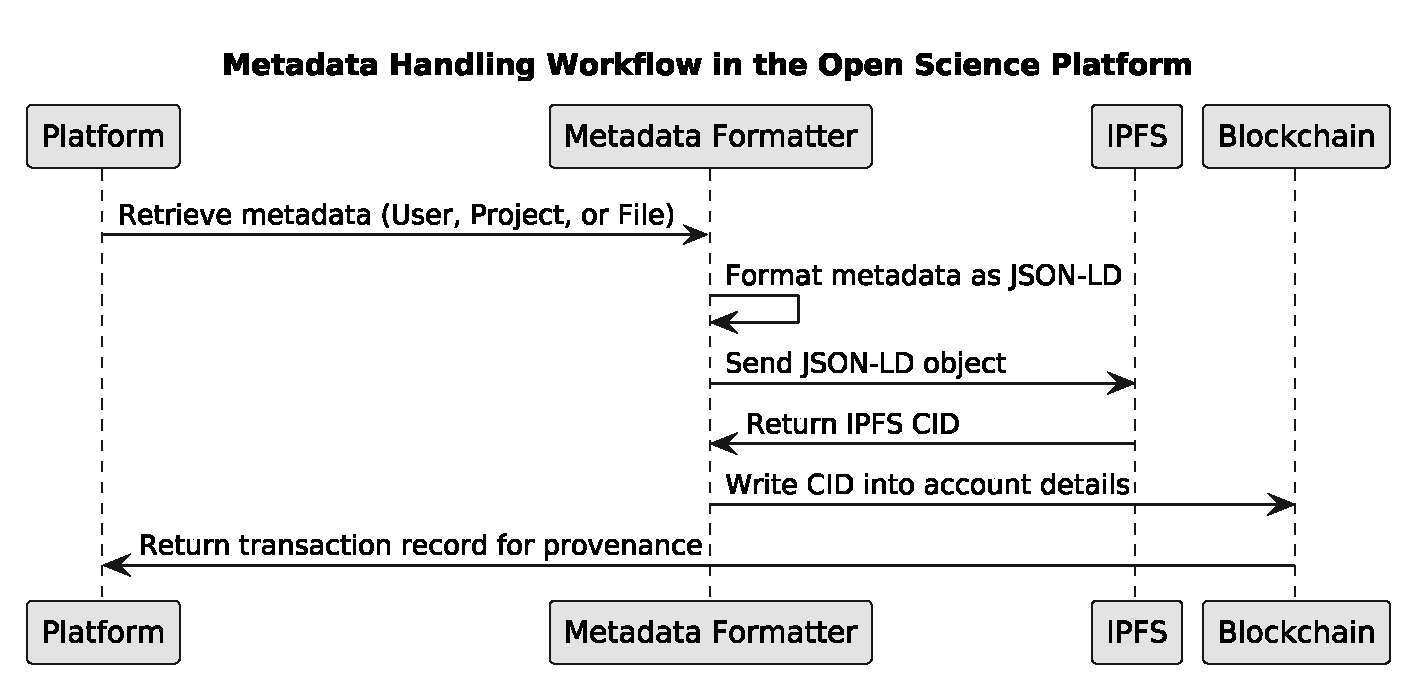
\includegraphics[width=0.98\textwidth, keepaspectratio]{fig/metadata_workflow_sequence.eps}
    \caption{General workflow for metadata handling in the Open Science Platform}
    \label{fig:metadata_workflow}
\end{figure}

\subsection{Blockchain Representation of Metadata}

In the Open Science platform, metadata for users, projects, and files are stored on the blockchain. This ensures the integrity and provenance of the metadata while leveraging decentralized technologies. The following subsections describe the structure of blockchain representations for both user and project data, as well as the files associated with these projects.

\subsection{User Account}

The representation of a user's account on the blockchain contains the standard Iroha v1 attributes for the account entity, such as the unique account identifier, domain information, and quorum for consensus. Additionally, the \texttt{json\_data} attribute references both the project to which the user is linked and the user's metadata CID (Content Identifier) stored on IPFS. This blockchain-based approach ensures that the user’s information remains immutable and traceable, which is critical for maintaining the integrity of research data.

Figures~\ref{fig:user_blockchain_representation} and~\ref{fig:user_bct_rep} presents the JSON structure for account details for a user in the Iroha v1 blockchain.

\begin{figure}[h]
    \centering
    \caption{Blockchain Representation of User Account}
    \label{fig:user_blockchain_representation}
    \begin{verbatim}
    {
        "account_id": "zealous_ptolemy@test",
        "domain_id": "test",
        "quorum": 1,
        "json_data": {
            "admin@test": {
                "linked_project": "02226@test",
                "account_metadata_cid": "QmT31fzDBNYAz1jAoAa7gQqSP7mDquv3fR8z1xLfxeHR5o"
            }
        }
    }
    \end{verbatim}
\end{figure}

\begin{figure}[htbp]
    \centering
    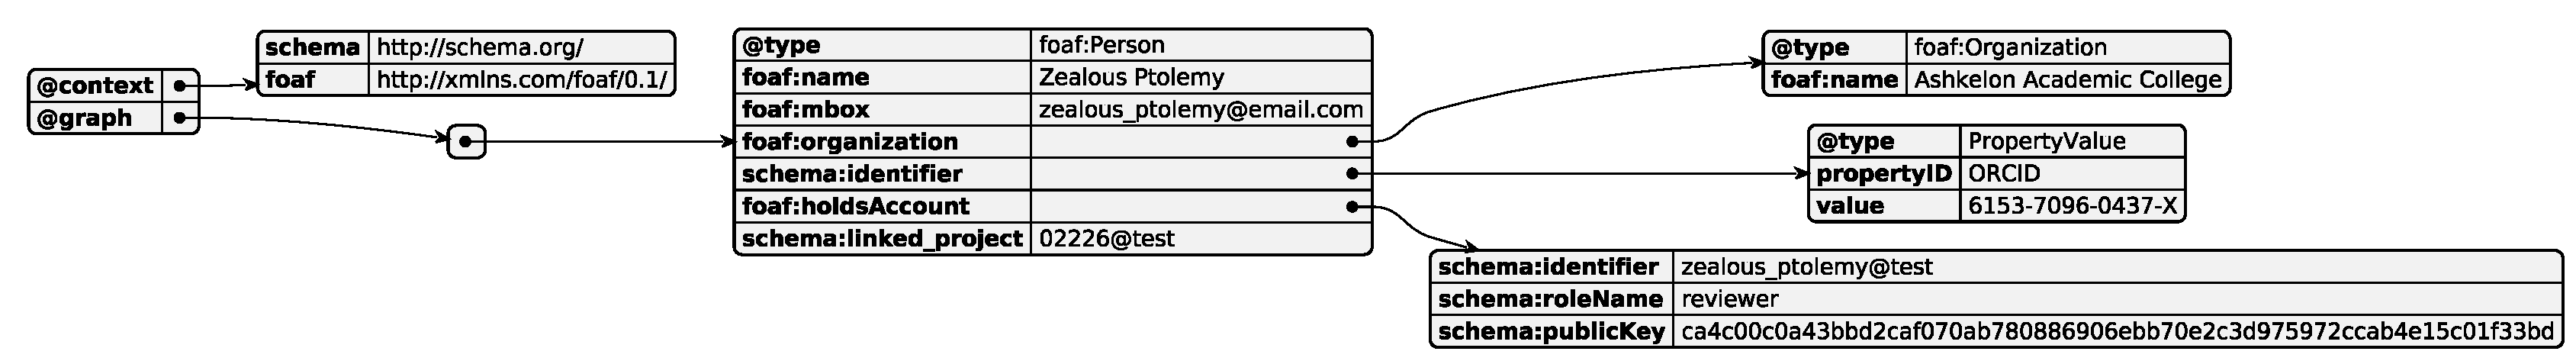
\includegraphics[width=0.98\textwidth, keepaspectratio]{fig/user_bct_representation.eps}
    \caption{User blockchain representation}
    \label{fig:user_bct_rep}
\end{figure}



\subsection{Project Account}

The project account representation similarly uses a blockchain-based structure to store project-related metadata. Each project is identified by a unique account ID, along with the project’s domain and quorum. The project metadata is linked to the user and includes important information about files associated with the project, including their CID references on IPFS. This ensures that the project data is linked to the user’s account and that all files and metadata related to the project are securely stored on the blockchain for provenance tracking.

The JSON structure describes the account details for a project in the Iroha v1 blockchain as shown in Figures~\ref{fig:project_blockchain_representation} and ~\ref{fig:project_bct_rep}.


\begin{figure}[h]
    \centering
    \caption{Blockchain Representation of Project Account}
    \label{fig:project_blockchain_representation}
    \begin{verbatim}
    {
        "account_id": "02226@test",
        "domain_id": "test",
        "quorum": 1,
        "json_data": {
            "admin@test": {
                "file_1": [
                    "QmTLZSqzPexwEdniZXLPN6fUfmEXX6MXS3b4QjKURgxc9y",
                    "Qmchg7At5whR1T4xP8TwTMd8ntQqJXbbSicJRtGGaW1Z2P"
                ],
                "linked_user": "zealous_ptolemy@test",
                "account_metadata_cid": "Qmay4cDaxUaZaHoJKqzN69XkiX8wMx17aG4VMmwmkLcL1a"
            }
        }
    }
    \end{verbatim}
\end{figure}


\begin{figure}[htbp]
    \centering
    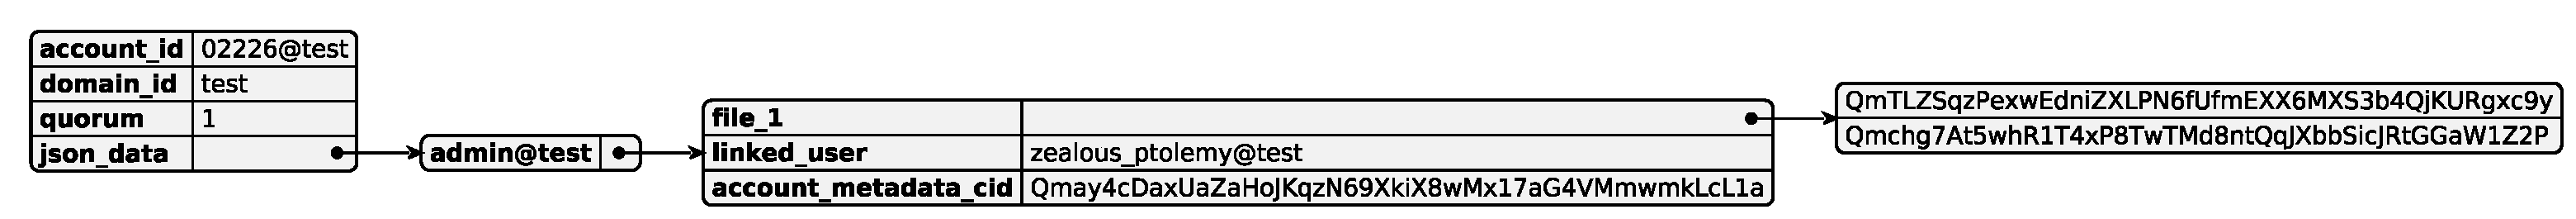
\includegraphics[width=0.98\textwidth, keepaspectratio]{fig/bct_user_representation.eps}
    \caption{Project blockchain representation}
    \label{fig:project_bct_rep}
\end{figure}



\subsection*{File Representation}

Within the project account, each file associated with the project is represented by a CID pair. The first CID refers to the file stored on IPFS, while the second CID references the metadata associated with that file. This structure ensures that the file's content and its metadata are both stored and tracked independently, but are still linked to the blockchain for integrity and provenance.

\begin{itemize}
    \item The \textbf{first CID} (\texttt{QmTLZSqzPexwEdniZXLPN6fUfmEXX6MXS3b4QjKURgxc9y}) corresponds to the \textbf{file}.
    \item The \textbf{second CID} (\texttt{Qmchg7At5whR1T4xP8TwTMd8ntQqJXbbSicJRtGGaW1Z2P}) corresponds to the \textbf{metadata of the file}, ensuring that all relevant details are retrievable.
\end{itemize}

This structure allows for the efficient tracking and retrieval of research project data while maintaining provenance and integrity through blockchain storage.

\subsection{Provenance in the Open Science Platform}

The provenance system takes a two-fold approach, with both methods being native features of their respective systems. The first approach leverages Iroha v1’s transaction logging capabilities, where each transaction is recorded with a hexadecimal hash and timestamp. This provides a reliable mechanism for tracking the evolution of account states over time. The hash acts as a snapshot, allowing for the retrieval of any past state of an account based on the corresponding transaction hash, as depicted in in Figure~\ref{fig:provenance}.

The second approach makes use of IPFS’s native feature of Content Identifiers (CIDs) to track metadata associated with accounts, projects, and files. Each piece of metadata is linked to a unique CID, which allows for decentralized storage and immutability. A mismatch of the CID indicates that the metadata or file has been modified, ensuring the integrity of the information over time.

Together, these two approaches, transaction logging through Iroha v1’s blockchain and metadata tracking through IPFS CIDs, provide a robust and transparent provenance system, ensuring both the transaction history and the integrity of metadata are verifiably recorded and traceable.


\begin{figure}[htbp]
    \centering
    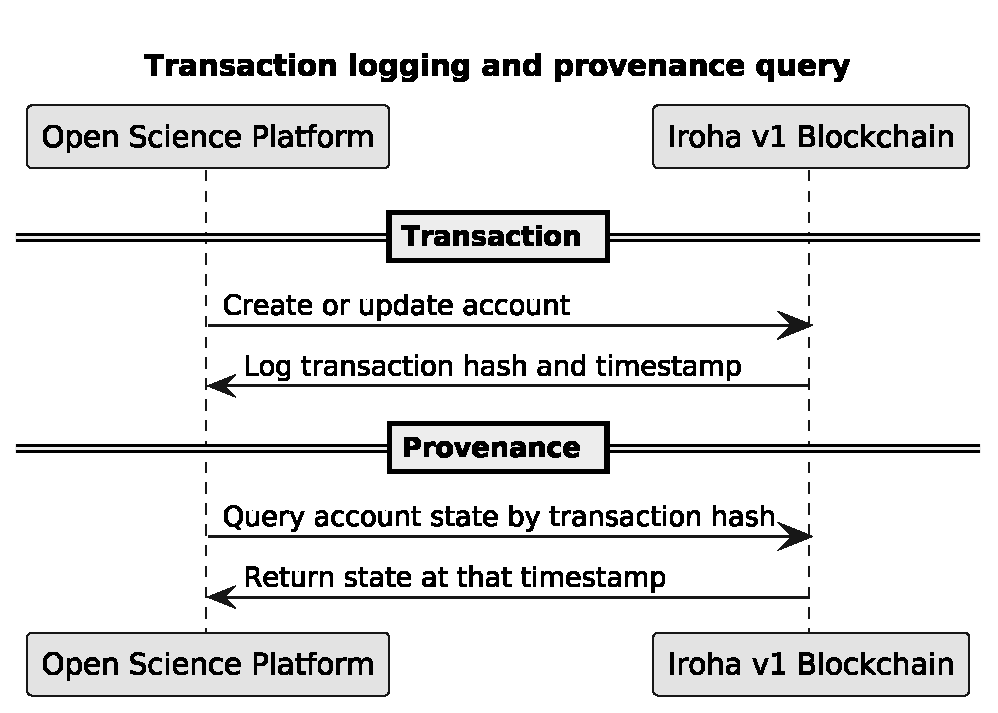
\includegraphics[width=0.98\textwidth, keepaspectratio]{fig/provenance_timeline.eps}
    \caption{Transaction logging and provenance query}
    \label{fig:provenance}
\end{figure}



%-------------------------------------------------------------
\section{Summary}
\label{sec:experiments:summary}
%-----------------------

This chapter presents the Open Science Platform that provides a comprehensive and robust proposition for enhancing the reproducibility and transparency of scientific research. It leverages a modern technology stack comprising the Iroha v1 blockchain, InterPlanetary File System (IPFS), Jupyter Notebooks, Apache Tika, and Woosh. This stack ensures secure and efficient management of data and artifacts across the platform. The Iroha v1 blockchain, integrated with smart contracts and the Ethereum EVM compatible Hyperledger Burrow, guarantees the immutability and trustworthiness of all recorded actions, while IPFS enables decentralized storage of research data, ensuring scalability and resilience. Jupyter Notebooks serve as the primary front-end interface, providing an interactive environment for users to engage with research artifacts. Apache Tika facilitates the extraction and processing of metadata from various document types, while Woosh powers advanced search and indexing functionalities, improving data discoverability and retrieval.

Platform operations are streamlined and well-defined. User enrollment and project registration are handled seamlessly through the Iroha v1 blockchain, where both users and projects are registered as accounts. This facilitates the management of roles, permissions, and interactions within the platform, ensuring efficient tracking. Artifact management is integrated with the platform's metadata extraction system, allowing for the efficient storage and retrieval of research artifacts that are consistently linked to their respective provenance, reinforcing the auditability of scientific outputs. Additionally, the search and validation functionalities provide users with tools to find, and explore research data.

The data model, represented through an Entity-Relationship (ER) model, underpins the platform's data structure, offering a flexible and comprehensive approach to managing users, projects, metadata, and research artifacts. The role of metadata in the platform is crucial, as it is structured using well-established ontologies, including FOAF, Schema.org, and Dublin Core. These ontologies standardize the metadata representation, enabling interoperability and ensuring that all data is both machine-readable and discoverable. The integration of blockchain technology ensures that all metadata is transparently recorded, with the blockchain acting as a secure ledger for all metadata transactions, ensuring data integrity and facilitating trust in the platform. Provenance tracking is an essential aspect of the Open Science Platform, allowing for the tracing of data and results back to their origin, providing transparency, accountability, and enhancing the reproducibility of research.

Looking to the future, the Open Science Platform holds significant potential for further development. Ongoing efforts will focus on expanding the artifact management capabilities, integrating more advanced search functionalities, and enhancing the platform’s ability to handle multi-source research data. A key focus will be on improving interoperability with existing open science platforms and initiatives, ensuring seamless integration and data exchange across various systems. Additionally, the platform aims to incorporate blockchain-based incentive mechanisms to encourage active participation and adoption. By offering rewards and recognition for contributors and users, these mechanisms will help foster a collaborative and thriving research ecosystem, accelerating the platform's growth and encouraging wider use in the scientific community. The continued adoption of open standards and the enhancement of user experience will ensure the platform’s scalability and relevance within the broader open science ecosystem.

%====================================================================
\chapter{Conclusions}
\label{chp:conclusions}
%====================================================================

\begin{quotation}[British Philosopher (1902-1994)]{Karl Poper}
    Science is one of the very few human activities, \\
    perhaps the only one, \\
    where errors are systematically criticized and fairly often, in time, corrected.
\end{quotation}

% \section{Analysis of the Hypothesis: Decentralized Technologies and Open Science}

% \subsection{Introduction}

\drop The hypothesis that decentralized technologies such as Blockchain, smart contracts, and IPFS can foster Open Science initiatives and improve reproducibility in scientific research contrasts with the current state of Open Science implementations. This section explores the potential of decentralized technologies in transforming the Open Science landscape by addressing existing challenges related to transparency, reproducibility, and accessibility, and contrasting it with the limitations of current centralized systems in Open Science. Blockchain, smart contracts, and IPFS provide solutions to issues related to transparency, reproducibility, and data accessibility. However, the widespread adoption of these technologies will require overcoming significant technical, legal, and infrastructural barriers. Despite these challenges, the potential of decentralized technologies to reshape the Open Science landscape and improve research reproducibility is substantial.

%\subsection{Current Open Science Implementations and Centralized Systems}

Open Science initiatives have made significant strides in promoting transparency and accessibility, but they still rely heavily on centralized systems. These centralized platforms, including institutional repositories, open access journals, and collaborative research networks, are often controlled by publishers, research institutions, or governmental bodies. These centralized structures have a number of limitations:
\begin{itemize}
    \item \textbf{Data Access and Sharing}: Although Open Science promotes the free sharing of research data, many repositories remain under the control of specific institutions or publishers, imposing access restrictions or ownership claims on the research data \cite{Boulton2015}.
    \item \textbf{Reproducibility Issues}: Despite efforts to enhance reproducibility, many scientific studies remain difficult to replicate due to centralized data storage and insufficient methodological transparency \cite{Borgman2012}.
    \item \textbf{Funding and Incentives}: Current Open Science models struggle to provide adequate incentives for researchers to share data or methodologies, with limited mechanisms for crediting those who contribute to reproducibility or open data sharing \cite{Nosek2015}.
\end{itemize}

\subsection{Decentralized Technologies and Their Potential Impact on Open Science and Reproducibility}
In contrast, decentralized technologies such as Blockchain, smart contracts, and IPFS offer several advantages that could address the limitations of centralized Open Science implementations:
\begin{itemize}
    \item \textbf{Blockchain for Transparency and Trust}: Blockchain can provide an immutable and transparent record of research activities, including data creation, peer review, and publication. This could solve issues related to data manipulation and ensure the integrity of research outputs \cite{Piwowar2011}.
    \item \textbf{Smart Contracts for Automatic and Trustless Collaboration}: Smart contracts can automate agreements within research collaborations, ensuring that contributions are recognized and rewarded transparently. These contracts could also help automate access permissions and licensing for research data \cite{Boulton2015}.
    \item \textbf{IPFS for Decentralized Data Storage}: IPFS enables decentralized storage, ensuring that research data remains accessible and tamper-proof, even if central servers become unavailable. This addresses long-term data accessibility and supports the open sharing of research data \cite{Borgman2012}.
\end{itemize}

\subsection{Improvement in Reproducibility}
While Open Science initiatives strive to improve reproducibility, several gaps remain:
\begin{itemize}
    \item \textbf{Data Accessibility}: Many research datasets are not freely available, and those that are often have access barriers, such as proprietary formats or storage restrictions in centralized repositories. Blockchain and IPFS provide mechanisms to ensure that data is permanently accessible and easy to replicate \cite{Leonelli2016}.
    \item \textbf{Methodological Transparency}: A significant barrier to reproducibility is insufficient detail on research methodologies. Blockchain could ensure that detailed methodologies, datasets, and code are publicly available and linked, increasing the transparency of research processes \cite{Piwowar2011}.
    \item \textbf{Incentives for Reproducibility}: The current Open Science framework lacks sufficient mechanisms for crediting and incentivizing researchers who engage in replication studies. Smart contracts can offer financial or academic rewards for reproducibility efforts, addressing this gap and encouraging more researchers to engage in replication \cite{Nosek2015}.
\end{itemize}

\subsection{Contrasts with Current Open Science Implementations}
The hypothesis that decentralized technologies could improve Open Science and reproducibility contrasts with the current state in several important ways:

\begin{itemize}
    \item \textbf{Centralization vs. Decentralization}: Current Open Science systems are largely centralized, creating reliance on specific institutions or publishers. Decentralized technologies offer a more robust and distributed infrastructure for data storage, collaboration, and verification, addressing the risks of central control.
    \item \textbf{Transparency and Integrity}: While transparency is a core principle of Open Science, centralized platforms can be susceptible to data manipulation and selective publishing. Blockchain can guarantee the integrity of research data and processes, providing a permanent, transparent, and auditable record of scientific activities.
    \item \textbf{Reproducibility and Data Sharing}: Decentralized systems such as IPFS allow for true open access and sharing of research data, ensuring that datasets remain accessible over time, even if central repositories are removed or discontinued. In comparison, centralized systems face limitations in long-term data storage and access.
    \item \textbf{Automation and Incentives}: Current Open Science platforms lack comprehensive mechanisms for automating research agreements or ensuring that researchers are properly incentivized for sharing data or conducting reproducibility studies. Smart contracts can automate the attribution of contributions, ensuring transparency and recognition in research collaborations.
\end{itemize}


\subsection{Section Summary}
The hypothesis that decentralized technologies can foster Open Science initiatives and improve reproducibility presents a promising contrast to the current limitations of centralized Open Science systems. Blockchain, smart contracts, and IPFS provide solutions to issues related to transparency, reproducibility, and data accessibility. However, the widespread adoption of these technologies will require overcoming significant technical, legal, and infrastructural barriers. Despite these challenges, the potential of decentralized technologies to reshape the Open Science landscape and improve research reproducibility is substantial.


As future directions, decentralized technologies have the potential to address many of the challenges faced by Open Science, several barriers remain:
\begin{itemize}
    \item \textbf{Adoption and Integration}: The integration of Blockchain, smart contracts, and IPFS into existing Open Science systems will require significant changes to infrastructure and researcher behavior. Many researchers may be hesitant to adopt new technologies due to unfamiliarity or concerns about the complexity of implementation \cite{Leonelli2016}.
    \item \textbf{Regulatory and Legal Issues}: Decentralized technologies raise important legal concerns, such as intellectual property protection, data privacy, and the enforcement of ethical standards. These challenges must be addressed before decentralized technologies can be widely adopted in scientific research \cite{Borgman2012}.
    \item \textbf{Scalability and Cost}: The scalability of decentralized technologies, especially Blockchain, may pose challenges when handling large volumes of data or complex computations. Additionally, the energy consumption and transaction costs associated with Blockchain could become limiting factors for widespread adoption in scientific research \cite{Boulton2015}.
\end{itemize}

\todo{Insert table - Causes and Impacts of the Reproducibility Crisis, see tables.tex}
\todo{Insert table: Summary of Reviewed Articles, see tables.tex}
\todo{Insert table: Cross-Cutting Themes and Blockchain Applications, see tables.tex}
\todo{Review captions and labels in tables}
\todo{Review chapter sections and subsections}
\todo{Review Conclusion and Summaries}
\todo{Review Cover}
\todo{Double-check references}


\backmatter

% Appendices would be placed here	


\makeback{./Bibliography}


\end{document}
